\PassOptionsToPackage{unicode=true}{hyperref} % options for packages loaded elsewhere
\PassOptionsToPackage{hyphens}{url}
%
\documentclass[]{book}
\usepackage{lmodern}
\usepackage{amssymb,amsmath}
\usepackage{ifxetex,ifluatex}
\usepackage{fixltx2e} % provides \textsubscript
\ifnum 0\ifxetex 1\fi\ifluatex 1\fi=0 % if pdftex
  \usepackage[T1]{fontenc}
  \usepackage[utf8]{inputenc}
  \usepackage{textcomp} % provides euro and other symbols
\else % if luatex or xelatex
  \usepackage{unicode-math}
  \defaultfontfeatures{Ligatures=TeX,Scale=MatchLowercase}
\fi
% use upquote if available, for straight quotes in verbatim environments
\IfFileExists{upquote.sty}{\usepackage{upquote}}{}
% use microtype if available
\IfFileExists{microtype.sty}{%
\usepackage[]{microtype}
\UseMicrotypeSet[protrusion]{basicmath} % disable protrusion for tt fonts
}{}
\IfFileExists{parskip.sty}{%
\usepackage{parskip}
}{% else
\setlength{\parindent}{0pt}
\setlength{\parskip}{6pt plus 2pt minus 1pt}
}
\usepackage{hyperref}
\hypersetup{
            pdftitle={A Guide through the People Analytics Lifecycle},
            pdfauthor={Craig Starbuck},
            pdfborder={0 0 0},
            breaklinks=true}
\urlstyle{same}  % don't use monospace font for urls
\usepackage{color}
\usepackage{fancyvrb}
\newcommand{\VerbBar}{|}
\newcommand{\VERB}{\Verb[commandchars=\\\{\}]}
\DefineVerbatimEnvironment{Highlighting}{Verbatim}{commandchars=\\\{\}}
% Add ',fontsize=\small' for more characters per line
\usepackage{framed}
\definecolor{shadecolor}{RGB}{248,248,248}
\newenvironment{Shaded}{\begin{snugshade}}{\end{snugshade}}
\newcommand{\AlertTok}[1]{\textcolor[rgb]{0.94,0.16,0.16}{#1}}
\newcommand{\AnnotationTok}[1]{\textcolor[rgb]{0.56,0.35,0.01}{\textbf{\textit{#1}}}}
\newcommand{\AttributeTok}[1]{\textcolor[rgb]{0.77,0.63,0.00}{#1}}
\newcommand{\BaseNTok}[1]{\textcolor[rgb]{0.00,0.00,0.81}{#1}}
\newcommand{\BuiltInTok}[1]{#1}
\newcommand{\CharTok}[1]{\textcolor[rgb]{0.31,0.60,0.02}{#1}}
\newcommand{\CommentTok}[1]{\textcolor[rgb]{0.56,0.35,0.01}{\textit{#1}}}
\newcommand{\CommentVarTok}[1]{\textcolor[rgb]{0.56,0.35,0.01}{\textbf{\textit{#1}}}}
\newcommand{\ConstantTok}[1]{\textcolor[rgb]{0.00,0.00,0.00}{#1}}
\newcommand{\ControlFlowTok}[1]{\textcolor[rgb]{0.13,0.29,0.53}{\textbf{#1}}}
\newcommand{\DataTypeTok}[1]{\textcolor[rgb]{0.13,0.29,0.53}{#1}}
\newcommand{\DecValTok}[1]{\textcolor[rgb]{0.00,0.00,0.81}{#1}}
\newcommand{\DocumentationTok}[1]{\textcolor[rgb]{0.56,0.35,0.01}{\textbf{\textit{#1}}}}
\newcommand{\ErrorTok}[1]{\textcolor[rgb]{0.64,0.00,0.00}{\textbf{#1}}}
\newcommand{\ExtensionTok}[1]{#1}
\newcommand{\FloatTok}[1]{\textcolor[rgb]{0.00,0.00,0.81}{#1}}
\newcommand{\FunctionTok}[1]{\textcolor[rgb]{0.00,0.00,0.00}{#1}}
\newcommand{\ImportTok}[1]{#1}
\newcommand{\InformationTok}[1]{\textcolor[rgb]{0.56,0.35,0.01}{\textbf{\textit{#1}}}}
\newcommand{\KeywordTok}[1]{\textcolor[rgb]{0.13,0.29,0.53}{\textbf{#1}}}
\newcommand{\NormalTok}[1]{#1}
\newcommand{\OperatorTok}[1]{\textcolor[rgb]{0.81,0.36,0.00}{\textbf{#1}}}
\newcommand{\OtherTok}[1]{\textcolor[rgb]{0.56,0.35,0.01}{#1}}
\newcommand{\PreprocessorTok}[1]{\textcolor[rgb]{0.56,0.35,0.01}{\textit{#1}}}
\newcommand{\RegionMarkerTok}[1]{#1}
\newcommand{\SpecialCharTok}[1]{\textcolor[rgb]{0.00,0.00,0.00}{#1}}
\newcommand{\SpecialStringTok}[1]{\textcolor[rgb]{0.31,0.60,0.02}{#1}}
\newcommand{\StringTok}[1]{\textcolor[rgb]{0.31,0.60,0.02}{#1}}
\newcommand{\VariableTok}[1]{\textcolor[rgb]{0.00,0.00,0.00}{#1}}
\newcommand{\VerbatimStringTok}[1]{\textcolor[rgb]{0.31,0.60,0.02}{#1}}
\newcommand{\WarningTok}[1]{\textcolor[rgb]{0.56,0.35,0.01}{\textbf{\textit{#1}}}}
\usepackage{longtable,booktabs}
% Fix footnotes in tables (requires footnote package)
\IfFileExists{footnote.sty}{\usepackage{footnote}\makesavenoteenv{longtable}}{}
\usepackage{graphicx,grffile}
\makeatletter
\def\maxwidth{\ifdim\Gin@nat@width>\linewidth\linewidth\else\Gin@nat@width\fi}
\def\maxheight{\ifdim\Gin@nat@height>\textheight\textheight\else\Gin@nat@height\fi}
\makeatother
% Scale images if necessary, so that they will not overflow the page
% margins by default, and it is still possible to overwrite the defaults
% using explicit options in \includegraphics[width, height, ...]{}
\setkeys{Gin}{width=\maxwidth,height=\maxheight,keepaspectratio}
\setlength{\emergencystretch}{3em}  % prevent overfull lines
\providecommand{\tightlist}{%
  \setlength{\itemsep}{0pt}\setlength{\parskip}{0pt}}
\setcounter{secnumdepth}{5}
% Redefines (sub)paragraphs to behave more like sections
\ifx\paragraph\undefined\else
\let\oldparagraph\paragraph
\renewcommand{\paragraph}[1]{\oldparagraph{#1}\mbox{}}
\fi
\ifx\subparagraph\undefined\else
\let\oldsubparagraph\subparagraph
\renewcommand{\subparagraph}[1]{\oldsubparagraph{#1}\mbox{}}
\fi

% set default figure placement to htbp
\makeatletter
\def\fps@figure{htbp}
\makeatother

\usepackage{booktabs}
\usepackage{etoolbox}
\makeatletter
\providecommand{\subtitle}[1]{% add subtitle to \maketitle
  \apptocmd{\@title}{\par {\large #1 \par}}{}{}
}
\makeatother
\usepackage[]{natbib}
\bibliographystyle{plainnat}

\title{A Guide through the People Analytics Lifecycle}
\providecommand{\subtitle}[1]{}
\subtitle{With Applications in R}
\author{Craig Starbuck}
\date{2022-02-27}

\begin{document}
\maketitle

{
\setcounter{tocdepth}{1}
\tableofcontents
}
\hypertarget{foreword}{%
\chapter{Foreword}\label{foreword}}

\hypertarget{intro}{%
\chapter{Introduction}\label{intro}}

Twenty years ago, I was the least likely person to write this book. My first statistics course in college was dreadful. On day one, my professor entered our large lecture hall of about 100 students and shared some grim stats: ``Based on historical data, half of you won't make it to the midterm and of those who do, half won't receive a passing grade in the end.'' This was both discouraging and motivating. Stats was a required course for my major so failure wasn't an option; I had to pass. The course was challenging, and I attended weekly study sessions with classmates and studied a lot independently to learn the material. I saw no applications for statistics to anything I planned to do with my degree, so the course was reduced to memorization of equations; it was not enjoyable. I passed the course with a B, and I was determined to never open another stats book.

You may be wondering what changed to motivate authoring a book involving this insufferable subject. The short answer is that I discovered the very important applications to a discipline I truly love, people analytics. The practical applications were altogether absent from my undergraduate statistics course. As I began to think about complex and nuanced challenges in social science contexts, it became clear that I would not only need to reengage with stats; I would need to develop an authentic appreciation for the discipline. Over the past decade, I have taken the journey of `relearning' statistics and developing a deep understanding of how statistical methodologies can be applied to various organizational problem statements.

My purpose in writing this book is to help make this content -- which may unfortunately be intimidating to many -- both accessible and exciting. In addition to my role in people analytics, I have taught a graduate-level business analytics course for Finance and MBA students for many years and have developed several teaching strategies through this experience that I will apply in this book. Beyond these instructional methods, this book makes a unique contribution in curating what I consider to be the most salient topics for people analytics practitioners. There are many texts available for deeper treatments of individual subjects covered in this book but as of this writing, I have found none that organize within a single text both theoretical and applied instruction spanning the whole of the people analytics lifecycle.

Thus, this book represents my earnest attempt to provide a concise -- yet adequately comprehensive -- treatment of the concepts and methods I've found to be most important for people analytics. My hope is that this book will ignite within you the same passion for analytics I have discovered over the past decade.

Craig Starbuck
December 2021

Craig Starbuck, PhD is the CEO and Co-Founder of OrgAcuity, a tech company with a mission to democratize access to people analytics. Craig has built and led people analytics teams at companies such as Robinhood, Mastercard, Equifax, TD Ameritrade, and Scottrade, and he also spent a decade in various data engineering and analytics positions in the banking and health care industries. He is a Member of the Society for Industrial and Organizational Psychology (SIOP) and has a passion for transforming people data into information and insights that help organizations enhance the experience and wellbeing of employees.

\hypertarget{planning}{%
\chapter{Project Planning}\label{planning}}

Nothing in this book will increase the value of an analysis no one needs. Analyses should always have a strong value proposition -- a clear expectation of how an analysis will support a General Manager, People Partner, Salesperson, or other member of the organization. Curiosity is not a business reason, and this chapter will cover a set of guiding principles as well as a project management framework that will help ensure analytics are anchored in well-defined problem statements with meaningful ROI.

In addition, this book will cut through the fluff and teach you how to do stuff that matters. Knowledge of concepts is futile without an understanding of how to apply them to people analytics use cases. Whether you are a people leader, individual contributor, or aspiring analytics practitioner, this book is for you. This book will serve as a guide through the analytics lifecycle, curating the key concepts and applications germane to common questions and hypotheses within people analytics.

\hypertarget{guiding-principles}{%
\section{Guiding Principles}\label{guiding-principles}}

Among the many principles guiding how analytics teams operate, there are three that I have found to be universally applicable and critical to the success of an analytics capability.

\hypertarget{pro-employee-thinking}{%
\subsection{Pro Employee Thinking}\label{pro-employee-thinking}}

``With Great Power Comes Great Responsibility.''

`Pro employee' thinking is addressed first and for good reason. People analytics has the power to improve the lives of people in meaningful ways. Whether we are shedding light on an area of the business struggling with work-life balance or identifying developmental areas of which a group of leaders may be unaware, people analytics ideally improves employee well-being and effectively, the success of the business. It is important to embrace a `pro employee' philosophy, as newfound knowledge could also have damaging repercussions if shared with the wrong people or if findings are disseminated without proper instruction on how to interpret and act.

One way to error on the side of caution when considering whether to disseminate insights is to ask the following: ``With this knowledge, could the recipient act in a manner that is inconsistent with our `pro employee' philosophy?'' If the answer to this question is not a clear ``no'', discuss with your HR, legal, and privacy partners and together, determine how best to proceed. The decision may be to not share the findings with the intended audience at all or to develop a proper communication and training plan to ensure there is consistency in how recipients interpret the insights and act in response. Employment Law and Data Privacy Counsel are our friends, and it is important to build strong relationships with these critical partners.

\hypertarget{quality}{%
\subsection{Quality}\label{quality}}

``Garbage In, Garbage Out.''

Never compromise quality for greater velocity. If quality falls to the bottom of the priority list, all other efforts are pointless. It is unlikely that requestors of data and analytics will ever ask us to take longer to prepare the information. The onus is on us as analytics professionals to level set on a reasonable timeline for analyses based on many factors that can materially impact the quality of analyses and insights. A single instance of compromised quality can have lasting damage on the reputation of the analytics function and cause consumers of insights to view all findings as suspect. Be sure quality is consistently a top value and guard your team's reputation at all costs. If stakeholders lose trust, there will likely be additional data requests for validation; this is wasteful to both you and your user community and detracts from the bigger story that needs to be conveyed.

To be clear, by `quality' I am referring to results, which is dependent on data integrity in the source systems, proper data preparation steps, and many other factors. Most of the analyst's time is spent on data preparation (data collection, cleaning and organizing, building training sets, mining for patterns, refining algorithms, etc.). If tight controls do not exist within the source application to support data integrity, data preparation efforts can only go so far in delivering reliable and valid findings. It is often the analysts who identify data integrity issues due to the nature of their work; therefore, close relationships should be formed with source application owners to put into place validation rules to proactively prevent the entry of erroneous data or at the very least, exception/audit reports to identify and address the issues soon after the fact.

\hypertarget{prioritization}{%
\subsection{Prioritization}\label{prioritization}}

``If everything is a priority, nothing is a priority.''

If there is not a supply-demand gap on the analytics team, the team likely isn't asking enough questions. It is okay (even good) to have a backlog of projects if unmet demand largely represents requests for lower-impact analyses. It is crucial to be relentless about prioritizing strategically important projects with `measurable' impact over merely interesting questions that few care to answer. According to the Pareto Principle, 80\% of outcomes (or outputs) result from 20\% of causes (or inputs). In analytics, it is important to be laser focused on identifying the 20\% of inputs that will result in disproportionate value creation for stakeholders. There are some general customer-oriented questions I have found to be helpful for the intake process to optimize the allocation of time and resources:

\begin{enumerate}
\def\labelenumi{\arabic{enumi}.}
\tightlist
\item
  Does this support a company or departmental objective? If not, why should this be prioritized over something else?
\item
  Who is the executive sponsor? Really important projects will have an executive-level sponsor.
\item
  What quantitative and/or qualitative data can be provided as a rationale for this request? Is there data to support doing this, or is the problem statement rooted merely in anecdotes?
\item
  Will this mitigate risk or enable opportunities?
\item
  What actions can or will be taken as a result of this analysis?
\item
  What is the \emph{scale} of impact (\# of impacted people)?
\item
  What is the \emph{depth} of impact (minimum --\textgreater{} significant)?
\item
  Is this a dependency or blocker for another important deliverable?
\item
  What is the impact of not doing (or delaying) this?
\item
  What is the request date? Is there flexibility in this date and/or scope of the request (e.g., what does MVP look like)?
\end{enumerate}

These questions can be weighted and scored as well to support a more automated and data-driven approach to prioritization.

\hypertarget{tools}{%
\section{Tools}\label{tools}}

This book uses freely available software for statistics, modeling, and data visualization. All code has been written such that it is fully reproducible should you choose to follow along on your machine (and I highly recommend you do).

\hypertarget{r}{%
\subsection{R}\label{r}}

While there are many commercial-grade analytics toolsets, R is open-sourced statistical and data visualization software that can be downloaded free of charge. It is incredibly powerful, and there is a package (or at least the ability to easily create one) for every conceivable statistical technique and data visualization. It is also widely used in highly regulated environments. As of this writing, R Markdown -- the dynamic document creator in which I am writing this book -- allows for coding in 56 different languages! Therefore, the debate around whether to use Python, Julia, or something else is now moot; we need not sacrifice the advantages of other languages by choosing one.

Please note that while R basics are covered, this is not a book on how to code. It is assumed that you already understand programming fundamentals. If this is not the case, an introductory programming course is highly recommended; this is one of the best investments you can make for a successful career in analytics. The ability to write code is now table stakes for anyone in an analytics-oriented field, as this is the best way to develop reproducible analyses. Coding is to analytics professionals what typing was for Baby Boomers decades ago; a lack of coding proficiency is a major limiting factor on one's potential in this field.

The goal of the code provided in this book is not to represent the most performant, succinct, or productionalizable approaches. The code herein is intended only to facilitate understanding and demonstrate how concepts can be implemented in people analytics settings. Programming expertise is important for optimizing these approaches for production applications.

\hypertarget{d-framework}{%
\section{4D Framework}\label{d-framework}}

In practical analytics settings, we generally operate with respect to five primary constraints: timeliness, client expectation, accuracy, reliability, and cost (Bartlett, 2013). Adherence to a lightweight framework over hastily rushing into an analysis full of assumptions generally lends to better outcomes that respect these constraints. A framework ensures (a) the problem statement is understood and well-defined; (b) relevant literature and prior research are reviewed; (c) the measurement strategy is sound; (d) the analysis approach is suitable for the hypotheses being tested; and (e) results and conclusions are valid and communicated in a way that resonates with the target audience. This chapter will outline a recommended framework as well as other important considerations that should be reviewed early in the project.

It is important to develop a clear understanding of the key elements of research. Scientific research is the systematic, controlled, empirical, and critical investigation of natural phenomena guided by theory and hypotheses about the presumed relations among such phenomena (Kerlinger \& Lee, 2000). In other words, research is an organized and systematic way of finding answers to questions. If you are in the business of analytics, I encourage you to think of yourself as a research scientist -- regardless of whether you are wearing a lab coat or have plans to publish.

As we will discover when exploring the laws of probability in a later chapter, there is a 1 in 20 chance of finding a significant result when none exists. Therefore, it is important to remain disciplined and methodical to protect against backward research wherein the researcher mines data for interesting relationships or differences and then develops hypotheses which they know the data support. There have been many examples of bad research over the years, which often presents in the form of p-hacking or data dredging: the act of finding data to confirm what the researcher wants to prove. This can occur by running an exhaustive number of experiments to find one that supports the hypothesis, or by using only a subset of data which features the expected patterning.

Academics at elite research institutions are often under immense pressure to publish in top-tier journals which have a track record of accepting new ground-breaking research over replication studies or unsupported hypotheses, and incentives have unfortunately influenced some to compromise integrity. As my PhD advisor told me many years ago, an unsupported hypothesis -- while initially disappointing given the exhaustive literature review that precedes its development -- is a meaningful empirical contribution given theory suggests the opposite should be true.

If you participated in a science fair as a child, you are likely already familiar with the scientific method. The scientific method is the standard scheme of organized and systematic inquiry, and this duly applies to people analytics practitioners in the promotion of robust analyses and recommendations.

\begin{figure}

{\centering 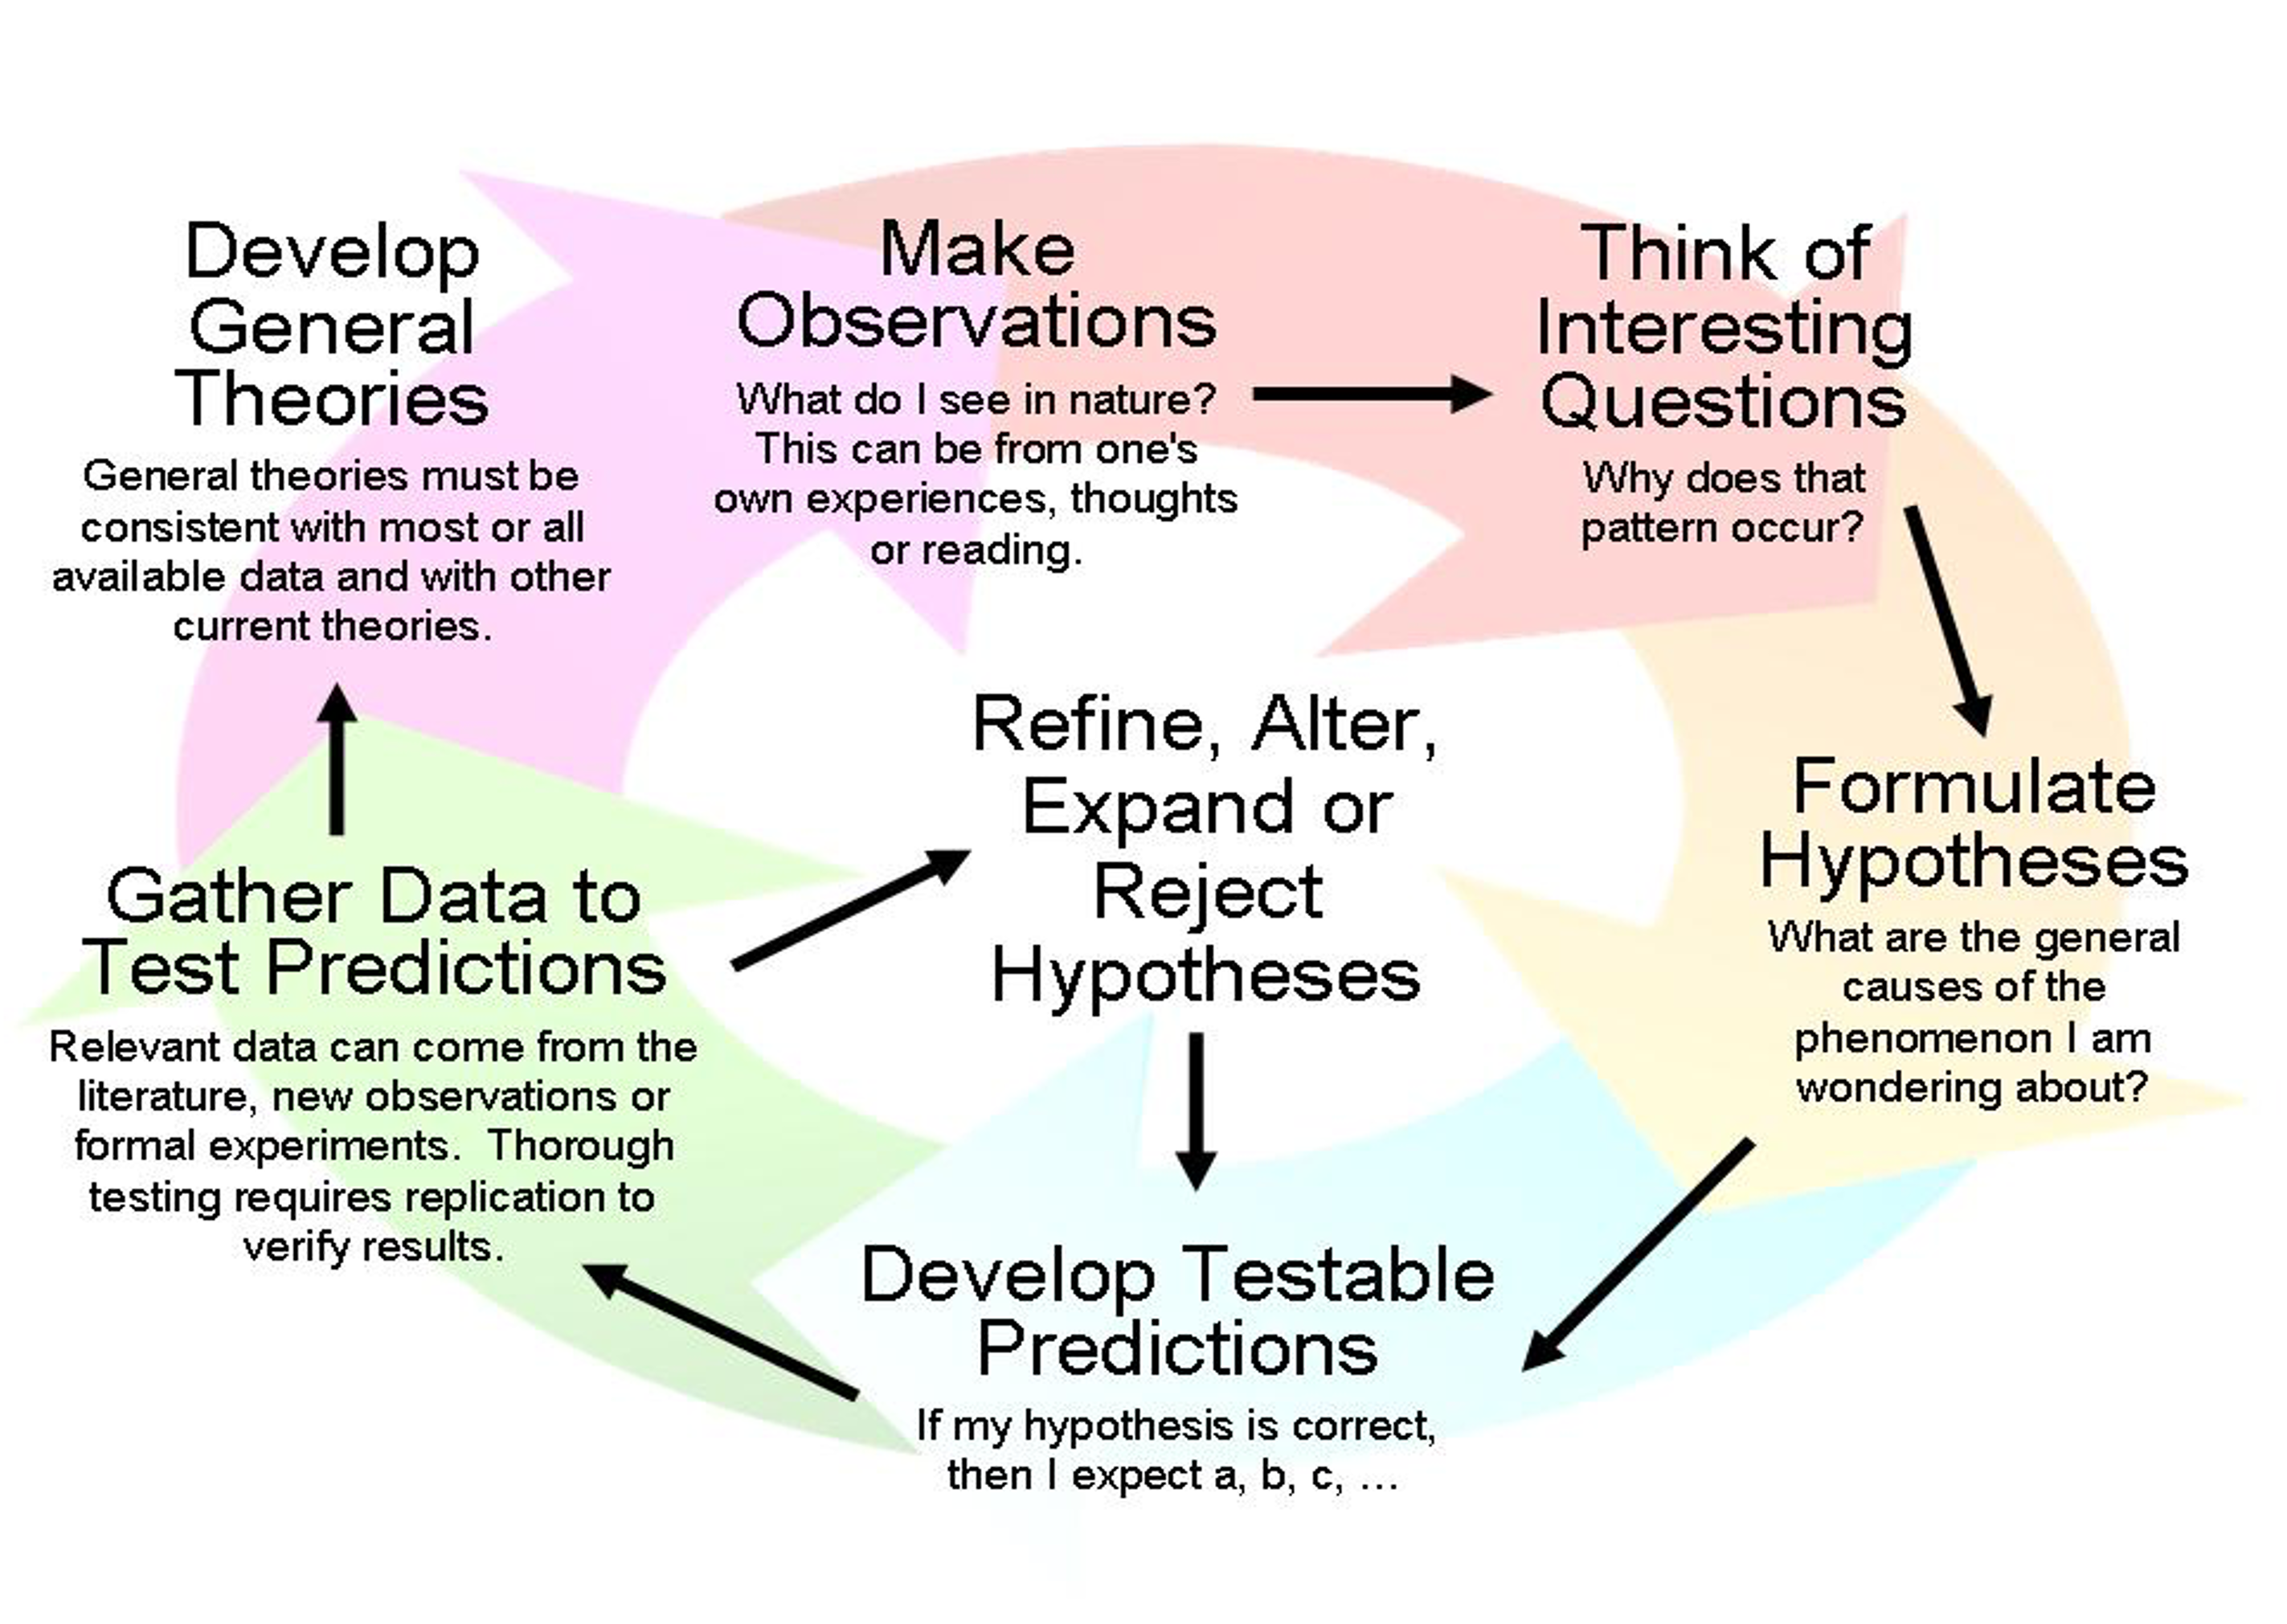
\includegraphics[width=0.75\linewidth]{/Users/craig.starbuck/Library/Mobile Documents/com~apple~CloudDocs/Documents/People Analytics Book/GitHub/peopleanalytics_lifecycle_book/graphics/scientific_method} 

}

\caption{The Scientific Method}\label{fig:sci-method}
\end{figure}

Over the years, I have adapted the scientific method into a curtailed four-dimensional framework which is intended to elevate the rigor applied to the end-to-end analytical process. The four dimensions are (a) Discover, (b) Design, (c) Develop, and (d) Deliver, and this book will be organized around these. A comprehensive checklist with questions and considerations for each phase of the analytics lifecycle can be found in the Appendix.

\begin{figure}

{\centering 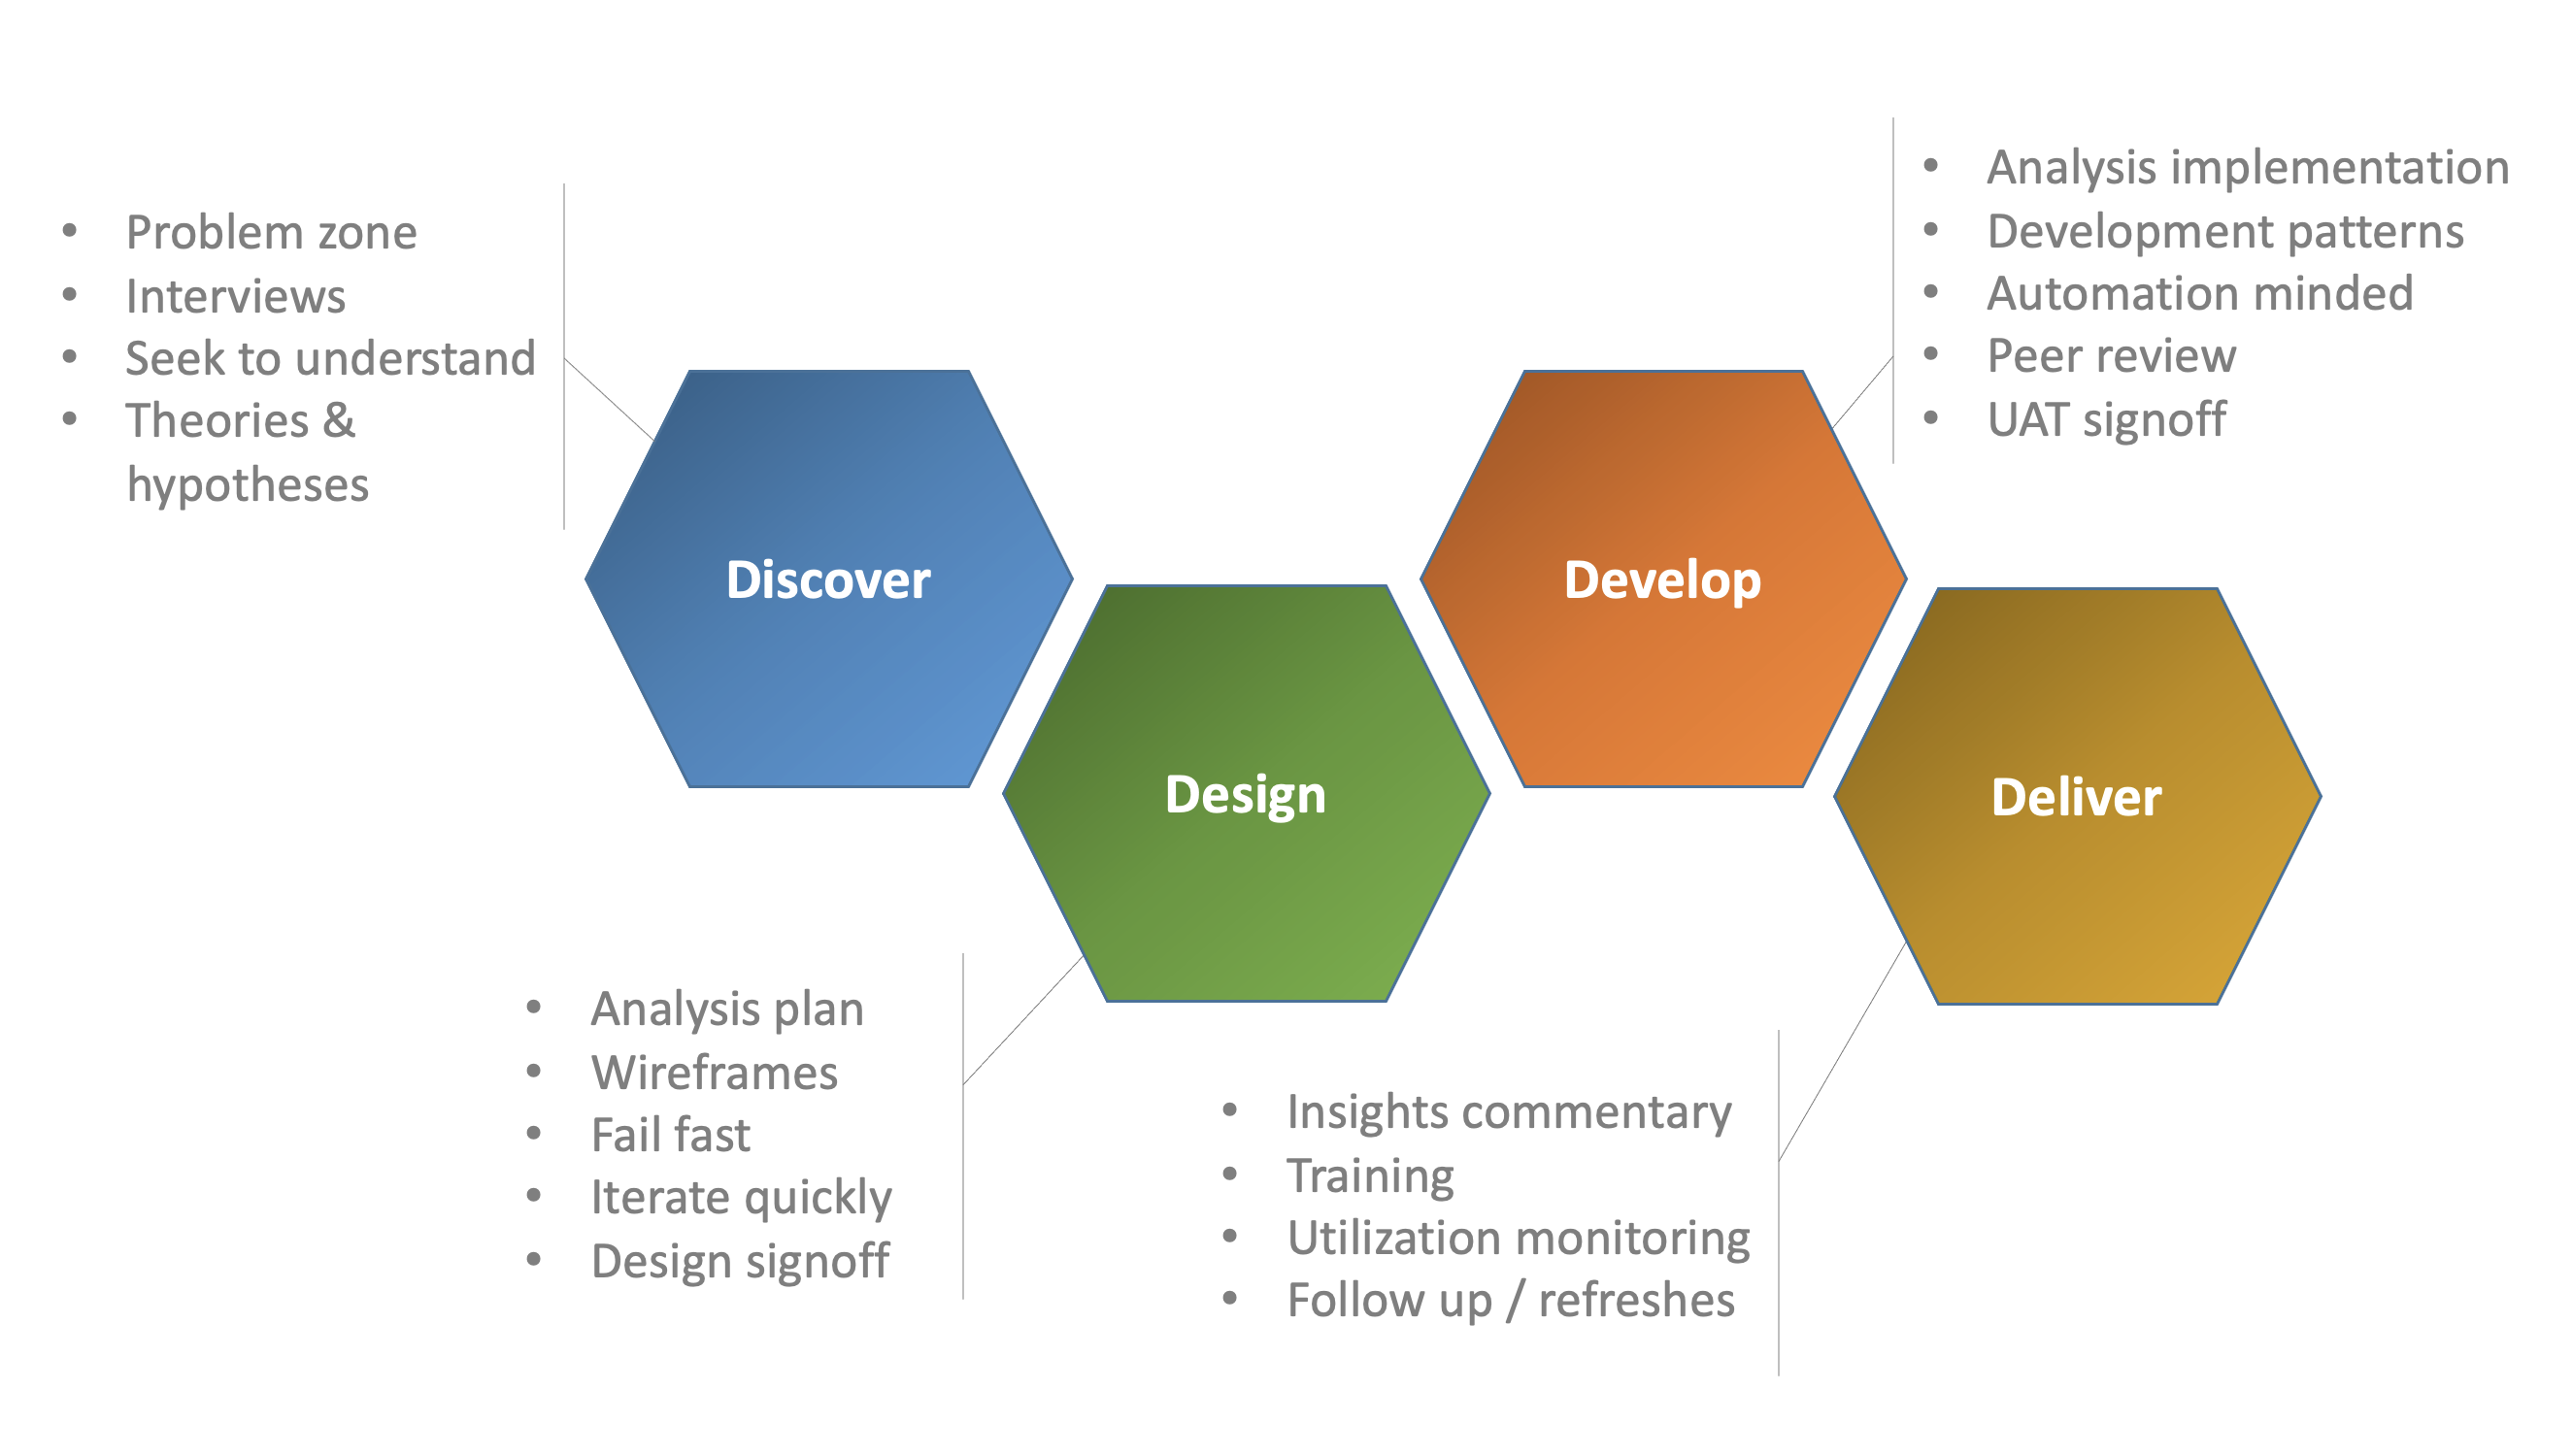
\includegraphics[width=1\linewidth]{/Users/craig.starbuck/Library/Mobile Documents/com~apple~CloudDocs/Documents/People Analytics Book/GitHub/peopleanalytics_lifecycle_book/graphics/4d_framework_overview} 

}

\caption{4D Framework}\label{fig:4d-framework}
\end{figure}

\hypertarget{discover}{%
\subsection{Discover}\label{discover}}

You are likely familiar with the following adage: ``An ounce of prevention is worth a pound of cure.'' Such is the case with respect to planning in an analytics context. During the Discover phase, it is important to remain in the problem zone; seek to understand your clients' needs through active listening and questions. This is not the time for solutioning or committing to any specific deliverables or timelines. If the client's needs are ambiguous, proceeding without clarity is unlikely to result in a favorable outcome.

It is generally helpful to think about analytics solutions like a Product Owner thinks about the initial and subsequent releases of a commercial product. A \textbf{Minimum Viable Product (MVP)} is a version of the solution with the minimum number of features to be useful to early customers who can provide feedback for future enhancements. It is important to clarify that the MVP version of solutions has both a limited number of users and features and that this is antithetical to building solutions that seek to address every imaginable question for every possible user. Breaking down large projects into small sets of features that are easier to communicate and adopt provides space for agility and real-time adjustments to the product roadmap per user feedback.

\hypertarget{design}{%
\subsection{Design}\label{design}}

Perhaps the most important initial question to answer in the design phase is: ``Does anything already exist that addresses part, or all, of the client's objectives?'' If an existing solution will suffice, or a previous analysis can be easily refreshed with recent data, it may be possible to allocate time and resources elsewhere. If related or complimentary analyses have already been performed, they may accelerate new analyses.

The end-user experience is of paramount importance during the Design phase, as solutions should have a consistent look and feel regardless of who developed them. Defining and implementing design guidelines will ensure consistency across analytics projects, as well as within large projects in which multiple analysts are collaborating on various components of the solution.

\hypertarget{develop}{%
\subsection{Develop}\label{develop}}

While development patterns can vary widely across analytics teams, establishing a set of standards can pay dividends in the form of greater efficiency and reliability over time. Pattern-based development ensures analysts who were not involved in a particular project can access the code and easily and quickly understand each step of the analysis: data extraction --\textgreater{} wrangling --\textgreater{} cleaning --\textgreater{} analysis --\textgreater{} visualization.

This is one of the many reasons tools like Excel will not be covered in this book. Software like R and Python allows analysts to organize and annotate steps of the analytical process in a manner that is both logical and reproducible. In case it bears repeating, learning to code is likely the best investment one can make in the pursuit of a career in analytics.

\hypertarget{deliver}{%
\subsection{Deliver}\label{deliver}}

The Deliver phase can take many forms depending on the solution being released. If the solution is designed for a large user base, a series of recorded trainings may be in order so that there is a helpful reference for those unable to attend the live sessions or new joiners in the future. It is important to monitor success measures, which could be insights aligned to research hypotheses, dashboard utilization metrics, progress following data-informed interventions, or any number of others defined within the Discover phase.

\hypertarget{r-intro}{%
\chapter{Introduction to R}\label{r-intro}}

This chapter covers how to install R, R Studio, and required packages for replicating examples in this book. This chapter also covers R basics such as objects, data structures, and data types that are fundamental to working in R.

\hypertarget{getting-started}{%
\section{Getting Started}\label{getting-started}}

Run and test your code frequently. Writing a significant number of lines before testing will make debugging your code far more difficult and time-intensive than it needs to be.

\textbf{Installing R}

R can be compiled and ran on a variety of platforms including UNIX, Windows, and MacOS. R can be downloaded here: \url{https://www.r-project.org/}

When installing R, you will need to select a CRAN mirror. The \textbf{Comprehensive R Archive Network (CRAN)} is a network of servers around the world that store identical, current versions of code and documentation for R. You should select the CRAN mirror nearest you to minimize network load.

\textbf{Installing R Studio}

\textbf{R Studio} is an \textbf{Integrated Development Environment (IDE)} for R. R Studio provides a console with syntax editing that is helpful for debugging code as well as tools for plotting, history, and workspace management. Both open source and commercial editions are available, but the open source option is sufficient for replicating everything in this book.

R Studio can be downloaded here: \url{https://www.rstudio.com/products/rstudio/download/\#download}

\textbf{Installing Packages}

Libraries from several R packages will be utilized in this book. The line of code below can be executed within R or R Studio to install all at once:

\begin{Shaded}
\begin{Highlighting}[]
\KeywordTok{install.packages}\NormalTok{(}\KeywordTok{c}\NormalTok{(}\StringTok{"tidyverse"}\NormalTok{, }\StringTok{"corrplot"}\NormalTok{, }\StringTok{"psych"}\NormalTok{, }\StringTok{"moments"}\NormalTok{, }\StringTok{"ggpubr"}\NormalTok{, }\StringTok{"GGally"}\NormalTok{), }\DataTypeTok{dependencies =} \OtherTok{TRUE}\NormalTok{, }\DataTypeTok{repos =} \StringTok{"http://cran.us.r-project.org"}\NormalTok{)}
\end{Highlighting}
\end{Shaded}

\begin{verbatim}
## 
##   There is a binary version available but the source version is later:
##          binary source needs_compilation
## corrplot   0.89   0.92             FALSE
## 
## 
## The downloaded binary packages are in
##  /var/folders/b1/0nnhbsx55hvfb1b3n83x0qrw0000gn/T//RtmpI3PY3R/downloaded_packages
\end{verbatim}

\textbf{Case Sensitivity}

It's important to note that everything in R is case-sensitive. When working with functions, be sure to match the case when typing the function name. For example, \texttt{Mean()} is not the same as \texttt{mean()}; since \texttt{mean()} is the correct case for the function, capitalized characters will result in an error when executing the function.

\textbf{Help}

Documentation for functions is available via the \texttt{?} command. This can be inserted prior to any function to access the function's documentation. For example, \texttt{?mean} will display the documentation, including its required and optional arguments, for the \texttt{mean()} function.

\textbf{Objects}

Objects underpin just about everything we do in R. An object is a container for various types of data. Objects can take many forms, ranging from simple objects holding a single number or character to complex structures that support advanced visualizations. The assignment character \texttt{\textless{}-} is used to assign values to an object.

Let's use the assignment operator to assign a number and character to separate objects. Note that non-numeric values must be enveloped in either single ticks \texttt{\textquotesingle{}\textquotesingle{}} or double quotes \texttt{""}:

\begin{Shaded}
\begin{Highlighting}[]
\NormalTok{obj_}\DecValTok{1}\NormalTok{ <-}\StringTok{ }\DecValTok{1}
\NormalTok{obj_}\DecValTok{1}
\end{Highlighting}
\end{Shaded}

\begin{verbatim}
## [1] 1
\end{verbatim}

\begin{Shaded}
\begin{Highlighting}[]
\NormalTok{obj_}\DecValTok{2}\NormalTok{ <-}\StringTok{ 'a'}
\NormalTok{obj_}\DecValTok{2}
\end{Highlighting}
\end{Shaded}

\begin{verbatim}
## [1] "a"
\end{verbatim}

Several functions are available for returning the type of data in an object:

\begin{Shaded}
\begin{Highlighting}[]
\KeywordTok{typeof}\NormalTok{(obj_}\DecValTok{2}\NormalTok{)}
\end{Highlighting}
\end{Shaded}

\begin{verbatim}
## [1] "character"
\end{verbatim}

\begin{Shaded}
\begin{Highlighting}[]
\KeywordTok{class}\NormalTok{(obj_}\DecValTok{2}\NormalTok{)}
\end{Highlighting}
\end{Shaded}

\begin{verbatim}
## [1] "character"
\end{verbatim}

\textbf{Comments}

The \texttt{\#} symbol is used for commenting/annotating code. This is a best practice to aid in quickly and easily deciphering the role of each line or block of code. Without comments, troubleshooting large scripts can be a more challenging task than necessary.

\begin{Shaded}
\begin{Highlighting}[]
\CommentTok{# Assign a new number to the object named obj_1}
\NormalTok{obj_}\DecValTok{1}\NormalTok{ <-}\StringTok{ }\DecValTok{2}
\CommentTok{# Display value in obj_1}
\NormalTok{obj_}\DecValTok{1}
\end{Highlighting}
\end{Shaded}

\begin{verbatim}
## [1] 2
\end{verbatim}

\begin{Shaded}
\begin{Highlighting}[]
\CommentTok{# Assign a new character to the object named obj_2}
\NormalTok{obj_}\DecValTok{2}\NormalTok{ <-}\StringTok{ 'b'}
\CommentTok{# Display value in obj_2}
\NormalTok{obj_}\DecValTok{2}
\end{Highlighting}
\end{Shaded}

\begin{verbatim}
## [1] "b"
\end{verbatim}

In-line code comments can also be added where needed to reduce the number of lines in a script:

\begin{Shaded}
\begin{Highlighting}[]
\CommentTok{# Assign a new number to the object named obj_1}
\NormalTok{obj_}\DecValTok{1}\NormalTok{ <-}\StringTok{ }\DecValTok{3}
\NormalTok{obj_}\DecValTok{1} \CommentTok{# Display value in obj_1}
\end{Highlighting}
\end{Shaded}

\begin{verbatim}
## [1] 3
\end{verbatim}

\begin{Shaded}
\begin{Highlighting}[]
\CommentTok{# Assign a new character to the object named obj_2}
\NormalTok{obj_}\DecValTok{2}\NormalTok{ <-}\StringTok{ 'c'} 
\NormalTok{obj_}\DecValTok{2} \CommentTok{# Display value in obj_2}
\end{Highlighting}
\end{Shaded}

\begin{verbatim}
## [1] "c"
\end{verbatim}

\hypertarget{vectors}{%
\section{Vectors}\label{vectors}}

A \textbf{vector} is the most basic data object in R. Vectors contain a collection of data elements of the same data type. For example, a vector may contain a series of numbers, and set of characters, or a collection of dates.

In this example, we introduce the combine function \texttt{c()}, which allows us to fill an object with more than one value:

\begin{Shaded}
\begin{Highlighting}[]
\CommentTok{# Create and fill a numeric vector named vect_num}
\NormalTok{vect_num <-}\StringTok{ }\KeywordTok{c}\NormalTok{(}\DecValTok{2}\NormalTok{,}\DecValTok{4}\NormalTok{,}\DecValTok{6}\NormalTok{,}\DecValTok{8}\NormalTok{,}\DecValTok{10}\NormalTok{)}
\NormalTok{vect_num}
\end{Highlighting}
\end{Shaded}

\begin{verbatim}
## [1]  2  4  6  8 10
\end{verbatim}

\begin{Shaded}
\begin{Highlighting}[]
\CommentTok{# Create and fill a character vector named vect_char}
\NormalTok{vect_char <-}\StringTok{ }\KeywordTok{c}\NormalTok{(}\StringTok{'a'}\NormalTok{,}\StringTok{'b'}\NormalTok{,}\StringTok{'c'}\NormalTok{)}
\NormalTok{vect_char}
\end{Highlighting}
\end{Shaded}

\begin{verbatim}
## [1] "a" "b" "c"
\end{verbatim}

We can use the \texttt{as.Date()} function to convert character strings containing dates to an actual date data type. By default, anything within single ticks or double quotes is treated as a character, so we must make an \textbf{explicit type conversion} from characters to dates. Remember that R is case-sensitive. Therefore, \texttt{as.date()} is not a valid function; the \texttt{D} must be capitalized.

\begin{Shaded}
\begin{Highlighting}[]
\CommentTok{# Create and fill a date vector named vect_dt}
\NormalTok{vect_dt <-}\StringTok{ }\KeywordTok{c}\NormalTok{(}\KeywordTok{as.Date}\NormalTok{(}\StringTok{"2021-01-01"}\NormalTok{), }\KeywordTok{as.Date}\NormalTok{(}\StringTok{"2022-01-01"}\NormalTok{))}
\NormalTok{vect_dt}
\end{Highlighting}
\end{Shaded}

\begin{verbatim}
## [1] "2021-01-01" "2022-01-01"
\end{verbatim}

We can use the sequence generation function \texttt{seq()} to fill values between a start and end point using a specified interval. For example, we can fill \texttt{vect\_dt} with the first day of each month between \texttt{2021-01-01} and \texttt{2022-01-01} via the \texttt{seq()} function and its \texttt{by\ =\ "months"} argument:

\begin{Shaded}
\begin{Highlighting}[]
\CommentTok{# Create and fill a date vector named vect_dt}
\NormalTok{vect_dt <-}\StringTok{ }\KeywordTok{seq}\NormalTok{(}\KeywordTok{as.Date}\NormalTok{(}\StringTok{"2021-01-01"}\NormalTok{), }\KeywordTok{as.Date}\NormalTok{(}\StringTok{"2022-01-01"}\NormalTok{), }\DataTypeTok{by =} \StringTok{'months'}\NormalTok{)}
\NormalTok{vect_dt}
\end{Highlighting}
\end{Shaded}

\begin{verbatim}
##  [1] "2021-01-01" "2021-02-01" "2021-03-01" "2021-04-01" "2021-05-01"
##  [6] "2021-06-01" "2021-07-01" "2021-08-01" "2021-09-01" "2021-10-01"
## [11] "2021-11-01" "2021-12-01" "2022-01-01"
\end{verbatim}

We can also use the \texttt{:} operator to fill integers between a starting and ending number:

\begin{Shaded}
\begin{Highlighting}[]
\CommentTok{# Create and fill a numeric vector with values between 1 and 10}
\NormalTok{vect_num <-}\StringTok{ }\DecValTok{1}\OperatorTok{:}\DecValTok{10}
\NormalTok{vect_num}
\end{Highlighting}
\end{Shaded}

\begin{verbatim}
##  [1]  1  2  3  4  5  6  7  8  9 10
\end{verbatim}

\textbf{Vectorized Operations}

\textbf{Vectorized operations (or vectorization)} underpin mathematical operations in R and greatly simplify computation. For example, if we need to perform a mathematical operation to each data element in a numeric vector, we do not need to specify each and every element explicitly. We can simply apply the operation at the vector level, and the operation will be applied to each of the vector's individual elements.

\begin{Shaded}
\begin{Highlighting}[]
\CommentTok{# Create a numeric vector named x and fill with values between 1 and 10}
\NormalTok{x <-}\StringTok{ }\DecValTok{1}\OperatorTok{:}\DecValTok{10}
\end{Highlighting}
\end{Shaded}

\begin{Shaded}
\begin{Highlighting}[]
\CommentTok{# Add 2 to each element of x}
\NormalTok{x_plus2 <-}\StringTok{ }\NormalTok{x}\OperatorTok{+}\DecValTok{2}
\NormalTok{x_plus2}
\end{Highlighting}
\end{Shaded}

\begin{verbatim}
##  [1]  3  4  5  6  7  8  9 10 11 12
\end{verbatim}

\begin{Shaded}
\begin{Highlighting}[]
\CommentTok{# Multiply each element of x by 2}
\NormalTok{x_times2 <-}\StringTok{ }\NormalTok{x}\OperatorTok{*}\DecValTok{2}
\NormalTok{x_times2}
\end{Highlighting}
\end{Shaded}

\begin{verbatim}
##  [1]  2  4  6  8 10 12 14 16 18 20
\end{verbatim}

\begin{Shaded}
\begin{Highlighting}[]
\CommentTok{# Square each element of x}
\NormalTok{x_sq <-}\StringTok{ }\NormalTok{x}\OperatorTok{^}\DecValTok{2}
\NormalTok{x_sq}
\end{Highlighting}
\end{Shaded}

\begin{verbatim}
##  [1]   1   4   9  16  25  36  49  64  81 100
\end{verbatim}

\hypertarget{matrices}{%
\section{Matrices}\label{matrices}}

A \textbf{matrix} is similar to a vector in that it represents a collection of data elements of the same data type; however, the elements of a matrix are \emph{arranged into a fixed number of rows and columns}.

We can create a matrix using the \texttt{matrix()} function. Per \texttt{?matrix}, the \texttt{nrow} and \texttt{ncol} arguments can be used to organize like data elements into a specified number of rows and columns.

\begin{Shaded}
\begin{Highlighting}[]
\CommentTok{# Create and fill matrix with numbers}
\NormalTok{mtrx_num <-}\StringTok{ }\KeywordTok{matrix}\NormalTok{(}\DataTypeTok{data =} \DecValTok{1}\OperatorTok{:}\DecValTok{10}\NormalTok{, }\DataTypeTok{nrow =} \DecValTok{5}\NormalTok{, }\DataTypeTok{ncol =} \DecValTok{2}\NormalTok{)}
\NormalTok{mtrx_num}
\end{Highlighting}
\end{Shaded}

\begin{verbatim}
##      [,1] [,2]
## [1,]    1    6
## [2,]    2    7
## [3,]    3    8
## [4,]    4    9
## [5,]    5   10
\end{verbatim}

We can leverage shorthand for function calls. As long as the argument values are in the correct order by the documentation, the argument names are not required. Per \texttt{?matrix}, the first argument is \texttt{data}, followed by \texttt{nrow} and then \texttt{ncol}. Therefore, we can achieve the same result using the following:

\begin{Shaded}
\begin{Highlighting}[]
\CommentTok{# Create and fill matrix with numbers}
\NormalTok{mtrx_num <-}\StringTok{ }\KeywordTok{matrix}\NormalTok{(}\DecValTok{1}\OperatorTok{:}\DecValTok{10}\NormalTok{, }\DecValTok{5}\NormalTok{, }\DecValTok{2}\NormalTok{)}
\NormalTok{mtrx_num}
\end{Highlighting}
\end{Shaded}

\begin{verbatim}
##      [,1] [,2]
## [1,]    1    6
## [2,]    2    7
## [3,]    3    8
## [4,]    4    9
## [5,]    5   10
\end{verbatim}

\hypertarget{factors}{%
\section{Factors}\label{factors}}

A \textbf{factor} is a data structure containing a finite number of categorical values. Each categorical value of a factor is known as a \textbf{level}, and the levels can be either ordered or unordered. This data structure is a requirement for several statistical models we will cover in later chapters.

We can create a factor using the \texttt{factor()} function:

\begin{Shaded}
\begin{Highlighting}[]
\CommentTok{# Create and fill factor with unordered categories}
\NormalTok{education <-}\StringTok{ }\KeywordTok{factor}\NormalTok{(}\KeywordTok{c}\NormalTok{(}\StringTok{"undergraduate"}\NormalTok{, }\StringTok{"post-graduate"}\NormalTok{, }\StringTok{"graduate"}\NormalTok{))}
\NormalTok{education}
\end{Highlighting}
\end{Shaded}

\begin{verbatim}
## [1] undergraduate post-graduate graduate     
## Levels: graduate post-graduate undergraduate
\end{verbatim}

Since education has an inherent ordering, we can use the \texttt{ordered} and \texttt{levels} arguments of the \texttt{factor()} function to order the categories:

\begin{Shaded}
\begin{Highlighting}[]
\CommentTok{# Create and fill factor with unordered categories}
\NormalTok{education <-}\StringTok{ }\KeywordTok{factor}\NormalTok{(education, }\DataTypeTok{ordered =} \OtherTok{TRUE}\NormalTok{, }\DataTypeTok{levels =} \KeywordTok{c}\NormalTok{(}\StringTok{"undergraduate"}\NormalTok{, }\StringTok{"graduate"}\NormalTok{, }\StringTok{"post-graduate"}\NormalTok{))}
\NormalTok{education}
\end{Highlighting}
\end{Shaded}

\begin{verbatim}
## [1] undergraduate post-graduate graduate     
## Levels: undergraduate < graduate < post-graduate
\end{verbatim}

The ordering of factors is critical to a correct interpretation of statistical model output as we will cover later.

\hypertarget{data-frames}{%
\section{Data Frames}\label{data-frames}}

\hypertarget{lists}{%
\section{Lists}\label{lists}}

\hypertarget{loops}{%
\section{Loops}\label{loops}}

\hypertarget{graphics}{%
\section{Graphics}\label{graphics}}

\hypertarget{user-defined-functions-udfs}{%
\section{User-Defined Functions (UDFs)}\label{user-defined-functions-udfs}}

\hypertarget{measure-sampl}{%
\chapter{Measurement \& Sampling}\label{measure-sampl}}

This chapter will survey the type and function of study variables, measurement scales, sampling and nonsampling error, as well as probability and nonprobability sampling methods.

\hypertarget{variable-types}{%
\section{Variable Types}\label{variable-types}}

The framing of variables in research hypotheses guides the treatment of each in our analyses. In this section, we will discuss the function of \emph{independent}, \emph{dependent}, \emph{control}, \emph{moderating}, and \emph{mediating} variables.

\hypertarget{independent-variables-iv}{%
\subsection{Independent Variables (IV)}\label{independent-variables-iv}}

An \textbf{Independent Variable (IV)} is a variable which is assumed to have a direct effect on another variable. IVs are sometimes referred to as \emph{predictors}, \emph{factors}, \emph{features}, \emph{antecedents}, or \emph{explanatory} variables.

For example, we may wish to examine whether an inclusion training program given to a random sample of leaders has a positive effect on team-level belonging. In a true experimental design, participation in the inclusion training would be the only difference between the treatment (teams whose leaders who participate in the training) and the control (teams whose leaders who do not participate in the training). In this case, inclusion training participation is the IV (the variable we are manipulating).

IVs are also present in non-experimental designs. For example, we may survey employees and ask them to rate their leader's inclusiveness and provide self-reported belonging ratings. In this context, leader inclusiveness (rather than an inclusion training) is the IV. If we find that average team-level belonging scores tend to be higher when leader inclusiveness scores are higher, this \emph{may} indicate that leader inclusion has some degree of influence on team-level belonging. Of course, there could be alternative explanations for any observed differences in team-level belonging, which is why experimental designs tend to provide stronger evidence for an IV's effect.

\hypertarget{dependent-variables-dv}{%
\subsection{Dependent Variables (DV)}\label{dependent-variables-dv}}

A \textbf{Dependent Variable (DV)} is a variable that is \emph{dependent} on the IV. DVs are also referred to as \emph{outcome}, \emph{response}, or \emph{criterion} variables.

In our leader inclusion example, team-level belonging is the DV since this variable is assumed to depend on the level of team leaders' inclusiveness. It's important to note that regardless of a study's results, it is the positioning of the variables in the study's hypotheses (rooted in theory) that determines the type of variable. If we hypothesize that leader inclusion training has a positive effect on team-level belonging, but the study finds no such effect, the inclusion intervention is still the IV and team-level belonging the DV.

\hypertarget{control-variables-cv}{%
\subsection{Control Variables (CV)}\label{control-variables-cv}}

A \textbf{Control Variable (CV)} is a variable that is held constant in research. The unchanging state of a CV allows us to understand the extent to which the IV has a unique and independent effect on the DV.

In an experimental context, control variables represent a researcher's attempt to control for alternative explanations so that the IV's main effect on the DV can be isolated. For example, in our leader inclusion example, to be confident that the reason for any observed differences in team-level belonging can be attributed to leader inclusion training rather than other factors that theoretically may explain differences. For example, we should ensure that the two groups are similar with respect to characteristics such as gender and ethnicity, since underrepresented groups (URGs) may have different experiences independent of any training programs. In this case, gender and ethnicity are CVs.

While we control for the effects of alternative explanations by way of the research design in an experimental context, we will discuss ways to control for these statistically in Chapter \ref{lm} for correlational designs. CVs are equally important in experimental and non-experimental contexts.

\hypertarget{moderating-variables}{%
\subsection{Moderating Variables}\label{moderating-variables}}

A \textbf{Moderating Variable} influences the strength of the effect of an IV on a DV. Moderating variables are often referred to as \emph{interactions} or \emph{interaction terms} in models.

Moderating variables may augment (strengthen) or attenuate (weaken) the effect one variable has on another. Interactions are widely understood in the context of medications; one drug may independently have a positive effect on one's health but when combined with another medication, the interaction can behave very differently -- and may even be lethal! In our inclusive leadership example, we may find that the strength of the training's effect on team-level belonging varies based on a leader's span of control (SoC). It stands to reason that leaders with a lower SoC may find it easier to cultivate a climate of inclusivity and belonging, while leaders with a higher SoC may have more scope/projects and team dynamics to manage and may find it more difficult to consistently apply strategies covered during the training.

Interactions between variables are vital to our understanding of nuance and complexity in the dynamics influencing outcomes in organizational settings. Chapter \ref{lm} will cover how to test for significant interactions.

\hypertarget{mediating-variables}{%
\subsection{Mediating Variables}\label{mediating-variables}}

A \textbf{Mediating Variable} explains the \emph{how} or \emph{why} of an IV's effect on a DV. It may be helpful to think of mediating variables as a ``go-between'' -- a part of the causal pathway of an effect.

In the case of inclusive leadership training, effects on belonging are likely not the result of the training itself. More likely, the training raised awareness and helped leaders develop strategies to help cultivate team inclusivity. One strategy endorsed during the training may be participative decision making, and the implementation of this strategy may explain \textbf{why} the training has a positive effect on team-level belonging. There may be multiple mediators of any observed effect of the intervention on team-level belonging depending on training outcomes.

Mediating variables may fully or partially mediate the relationship between an IV and DV. \textbf{Full mediation} indicates that the mediator fully explains the effect; in other words, without the mediator in the model, there is no relationship between an IV and DV. \textbf{Partial mediation} indicates that the mediator partially explains the effect; that is, there is still a relationship between an IV and DV without the mediator in the model. Partial mediation indicates that there are additional explanations for \emph{how} or \emph{why} observed effects exist, such as the implementation of additional team inclusion strategies influencing team belonging. In Chapter \ref{lm}, we will discuss how to test for both full and partial mediation.

Translating research hypotheses into conceptual models of hypothesized relationships is helpful in visually representing the function of each variable in the study. Figure \ref{fig:concept-mdl} illustrates how each type of variable is depicted using our inclusive leadership example:

\begin{figure}

{\centering 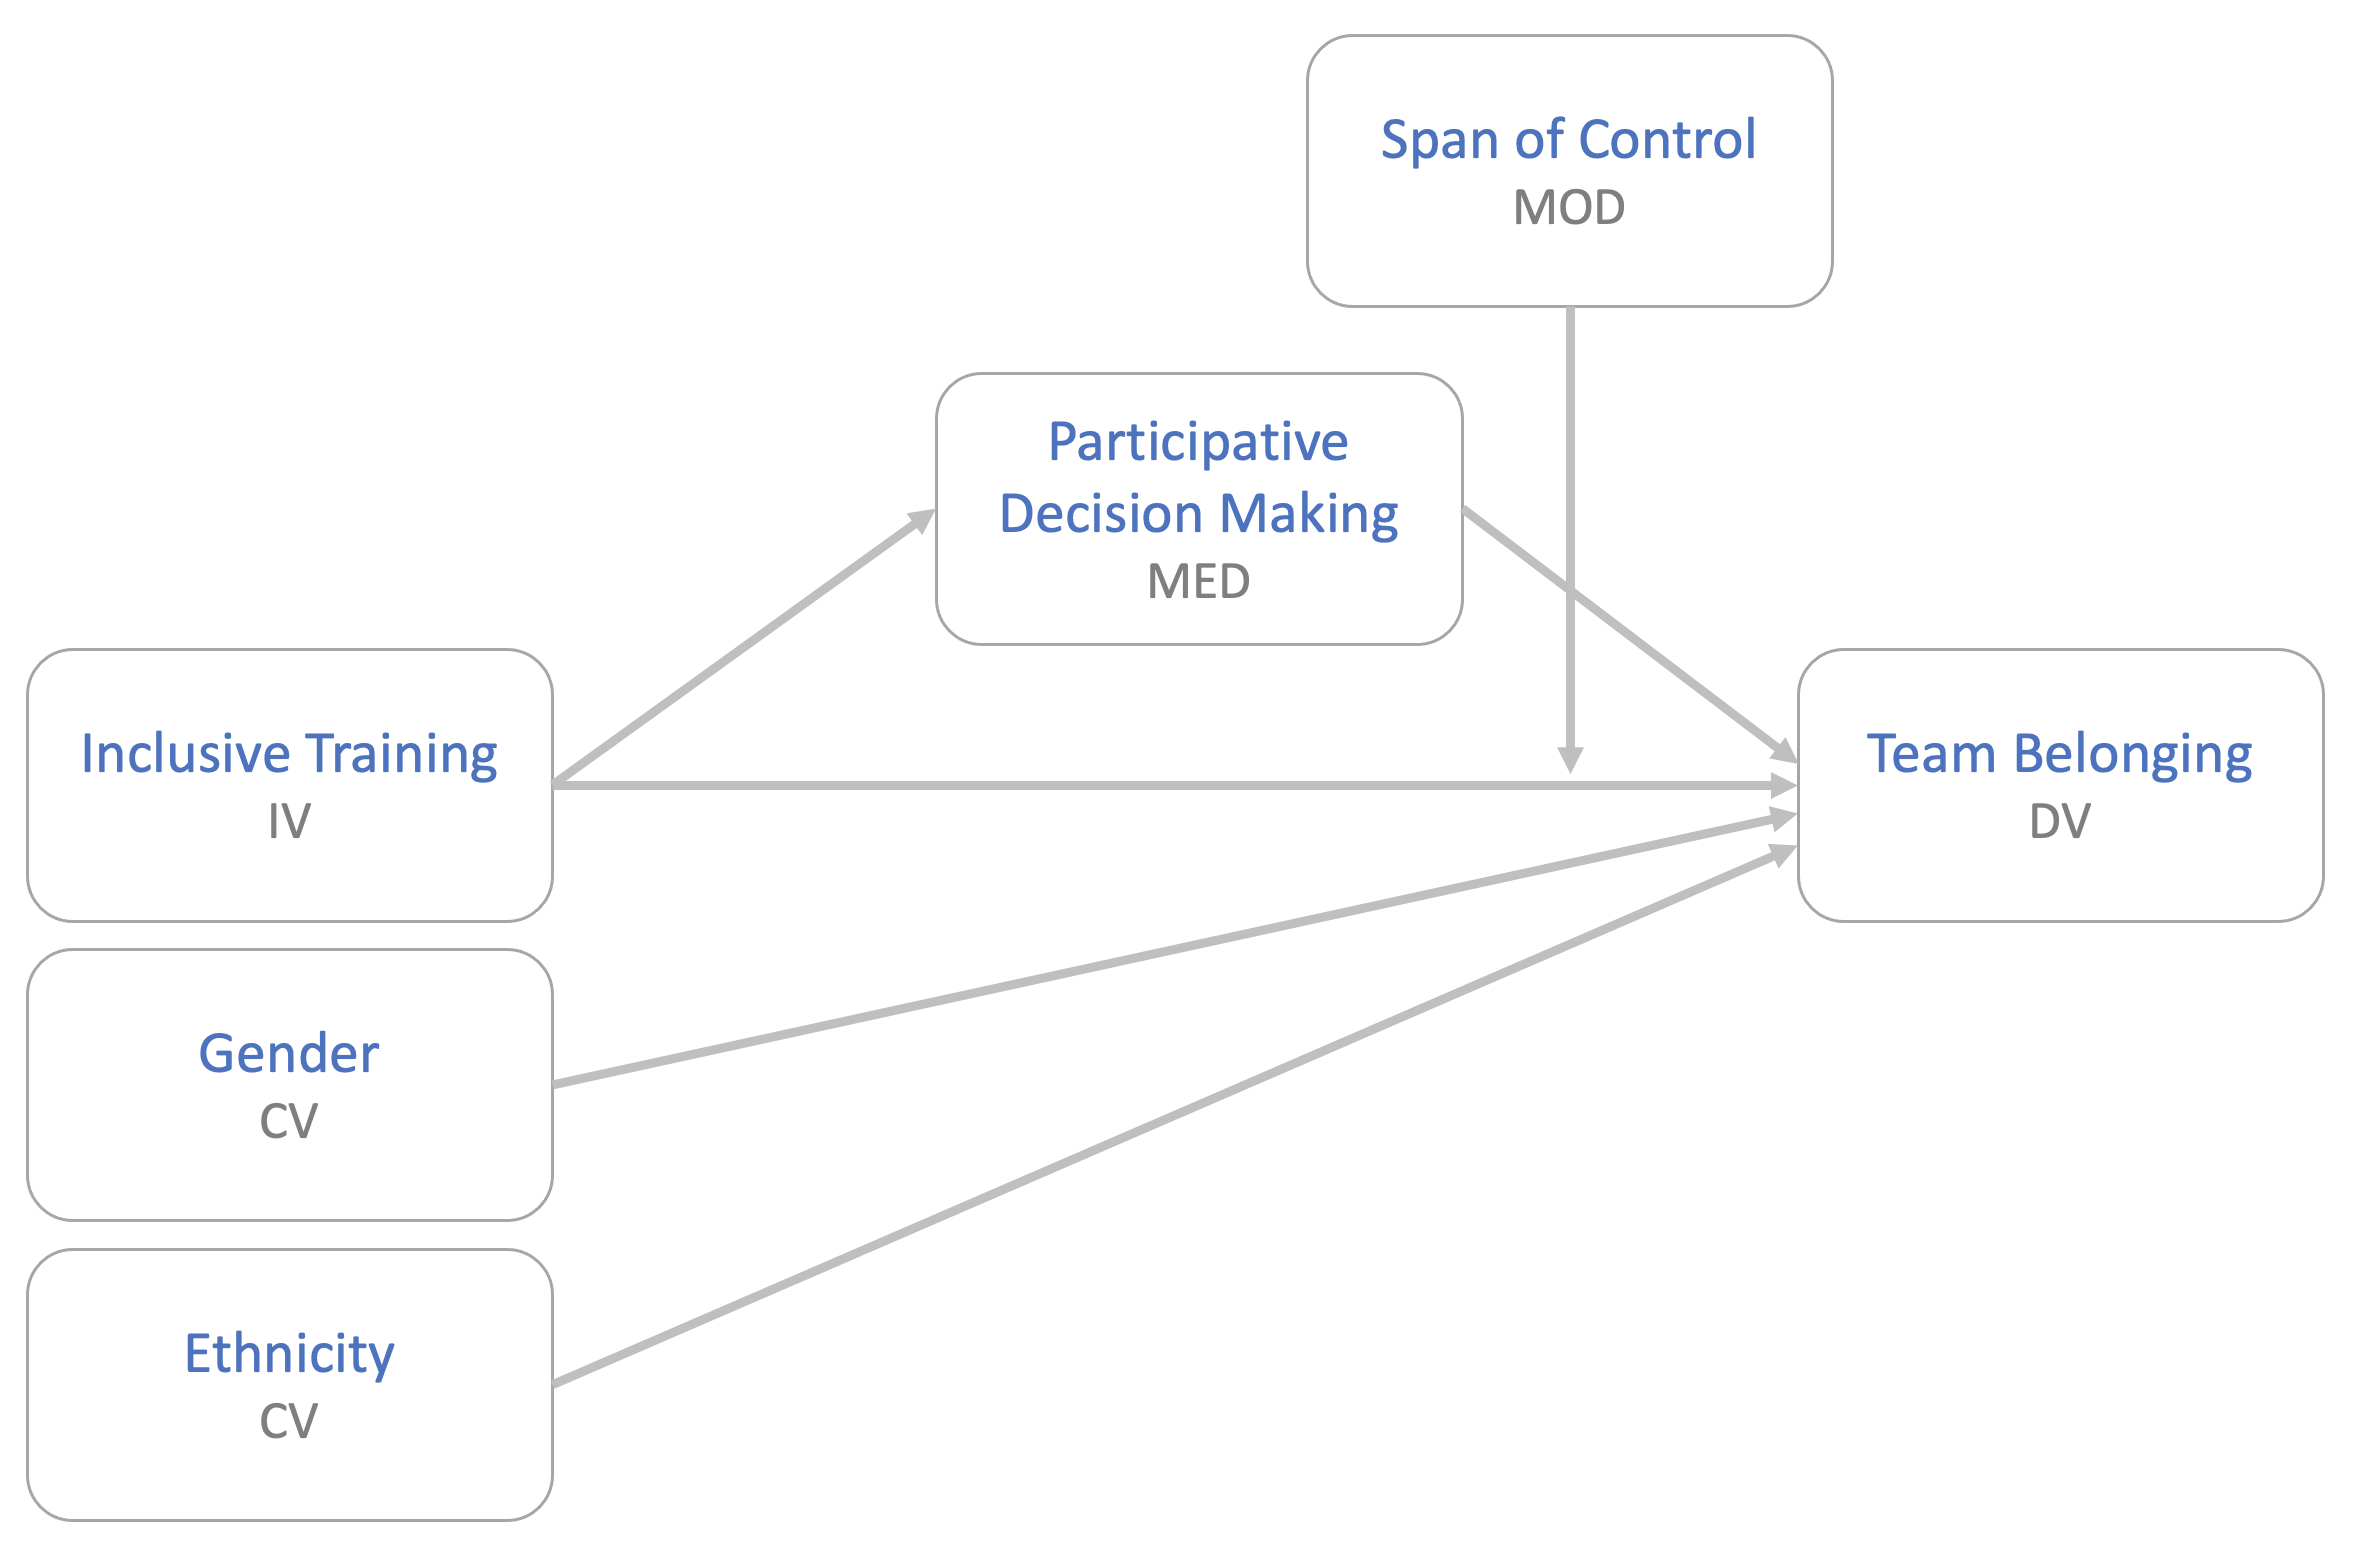
\includegraphics[width=0.75\linewidth]{/Users/craig.starbuck/Library/Mobile Documents/com~apple~CloudDocs/Documents/People Analytics Book/GitHub/peopleanalytics_lifecycle_book/graphics/conceptual_model} 

}

\caption{Conceptual Model of Hypothesized Relationships among Variables}\label{fig:concept-mdl}
\end{figure}

\hypertarget{measurement-scales}{%
\section{Measurement Scales}\label{measurement-scales}}

\textbf{Measurement scales} are used to categorize and quantify variables. There are two major categorizations -- \emph{discrete} and \emph{continuous} -- and these, together with the research hypotheses, help determine appropriate types of analyses to perform.

\hypertarget{discrete-variables}{%
\subsection{Discrete Variables}\label{discrete-variables}}

\textbf{Discrete variables} are also known as \emph{categorical} or \emph{qualitative} variables. Categorical variables have a finite or countable number of values associated with them, and these can be further categorized as either \emph{nominal} or \emph{ordinal}.

\textbf{Nominal}

A \textbf{nominal} variable is one with two or more categories for which there is no intrinsic ordering to the categories. Examples of nominal variables include office locations, departments, and teams. A \textbf{dichotomous variable} is a type of nominal variable which has only two unordered categories. Examples of dichotomous variables include people leader vs.~individual contributor, active vs.~inactive status, and remote worker vs.~non-remote worker.

\textbf{Ordinal}

An \textbf{ordinal} variable is similar to a nominal variable with one important difference: ordinal variables have \emph{ordered} categories. Examples of ordinal variables include education levels, job levels, and survey variables measured on Likert-type scales.

\hypertarget{continuous-variables}{%
\subsection{Continuous Variables}\label{continuous-variables}}

\textbf{Continuous variables} are also known as \emph{quantitative} variables. Continuous variables can assume any real value in some interval, and these can be further categorized as either \emph{interval} or \emph{ratio} variables.

\textbf{Interval}

Variables measured on an \textbf{interval} scale have a natural order and a quantifiable difference between values but no absolute zero value. Examples include SAT scores, IQ scores, and temperature measured in Fahrenheit or Celsius (but not Kelvin). In these examples, 0 is either not an option (i.e., SAT and IQ) or does not represent the absence of something (e.g., 0 degrees is a temperature, albeit a cold one!).

\textbf{Ratio}

Variables measured on a \textbf{ratio} scale have the same properties as data measured on an interval scale with one important difference: ratio data have an absolute zero value. Examples include compensation, revenue, and sales; a zero in these contexts is possible and would indicate a true absence of something.

\hypertarget{sampling}{%
\section{Sampling}\label{sampling}}

The goal of research is to understand a population based on data from a subset of population members. In practice, it is often not feasible to collect data from every member of a population, so we instead calculate \textbf{sample statistics} to estimate \textbf{population parameters}.

Another important concept is the \textbf{sampling frame}. While the population represents the entire group of interest, the sampling frame represents the subset of the population to which the researcher has access. In an ideal setting, the population and sampling frame are the same, but they are often different in practice. For example, a professor may be interested in understanding student sentiment about a new school policy but only has access to collect data from students in the courses she teaches. In this case, the entire student body is the population but the students she has access to (those in the courses she teaches) represent the sampling frame. The sample is the subset of the sampling frame that ultimately participates in the research (e.g,. those who complete a survey or participate in a focus group).

\hypertarget{sampling-nonsampling-error}{%
\subsection{Sampling \& Nonsampling Error}\label{sampling-nonsampling-error}}

Sampling and nonsampling errors are general categorizations of biases and error in research (Albright \& Winston, 2016).

\textbf{Sampling error} is the inevitable result of basing inferences on a random sample rather than the entire population. The two main contributors to sampling error are the size of the sample and variation in the underlying population. The risk of sampling error decreases as the sample size approaches the population size; however, it is usually not feasible to gain information from the entire population, so sampling error is generally a concern.

There are many types of \textbf{nonsampling error} that can invalidate results beyond the sampling procedure, and we will focus on several that are particularly germane to people analytics: \emph{nonresponse bias}, \emph{nontruthful responses}, \emph{measurement error}, and \emph{voluntary response bias}.

\textbf{Nonresponse Bias}

Surveys are a staple in the set of data sources germane to people analytics. While survey data provide unique attitudinal and perceptive signals that can be highly predictive of future behavior and events, surveys tend to be far more susceptible to nonsampling error than other data sources.

As discussed in the context of sampling error, we usually do not have access to information on entire populations of interest, so we must consider the possibility that those for whom we are missing data may have common qualities, perceptions, or opinions that differ from those for whom we do have data. This is known as \textbf{nonresponse bias}. For example, if we administer an employee experience survey to the entire organization and receive a 60\% response rate, the reality is that we do not know how the 40\% of nonrespondents would have responded. It is possible that nonrespondents represent highly disengaged employees, in which case their responses may have materially influenced results and conclusions in an unfavorable direction. It is also possible that the nonrespondents were busy, away on vacation, cynical to the confidentiality language in the communications, or any number of other reasons which may or may not have resulted in significantly different feedback from that of respondents.

Nonresponse bias is not limited to surveys. For example, self-reported demographics such as gender and ethnicity may not be disclosed by all employees in the HR information system (HRIS). This can bias segmentations based on these categorical dimensions. While there are strategies to address this, such as visual ID or applying models trained to infer missing values (which may be necessary to fulfill EEOC reporting requirements), there may still be error in the imputed values.

\textbf{Nontruthful Responses}

While high response rates may reduce nonresponse bias, this isn't always something to celebrate. Organizations that incentivize participation in surveys often do so at the risk of people responding in socially desirable ways and providing \textbf{nontruthful responses} to achieve some defined target. For example, if an employee has an unhealthy relationship with his manager but does not trust that managers will not have access to individual-level responses, the employee may decide to indicate on the survey that everything is highly favorable to help the team win the month of casual days leadership promised. This can of course skew and invalidate results.

While survey participation should be strongly encouraged since higher response rates can mitigate the risk of certain types of bias and increase confidence that the survey is representative of the collective organization's sentiments, incentivizing participation can be dangerous.

\textbf{Measurement Error}

\textbf{Measurement error} relates to errors stemming from confusing questions, survey fatigue, and low-quality scales used to measure multidimensional psychological constructs. The field of \textbf{psychometrics} is a vast scientific discipline concerned with the development of assessment tools, measurement instruments, and formalized models to understand latent psychological constructs such as engagement, belonging, purpose, and wellbeing using observable indicators.

The reduction of measurement error is a principal concern to psychometricians. For a deeper treatment of the survey scale development process, see DeVellis (2012). While an exhaustive treatment of psychometrics is beyond the scope of this book, \emph{reliability} and \emph{validity} are two broad sets of methods designed to increase the robustness of psychological instrumentation which will be reviewed in this section.

\begin{figure}

{\centering 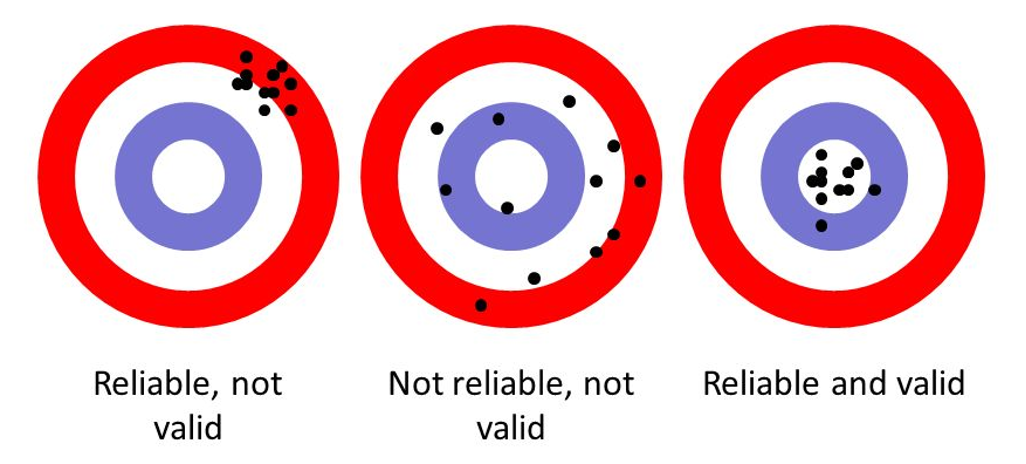
\includegraphics[width=0.75\linewidth]{/Users/craig.starbuck/Library/Mobile Documents/com~apple~CloudDocs/Documents/People Analytics Book/GitHub/peopleanalytics_lifecycle_book/graphics/reliability_validity} 

}

\caption{Reliability and Validity}\label{fig:reli-vali}
\end{figure}

\textbf{Reliability} describes the quality of measurement (i.e., the consistency or repeatability of measures). Types of reliability include:

\begin{itemize}
\tightlist
\item
  \textbf{Inter-Rater or Inter-Observer Reliability}: the degree to which different raters/observers give consistent estimates of the same phenomenon.
\item
  \textbf{Test-Retest Reliability}: the consistency of a measure from one time to another.
\item
  \textbf{Parallel-Forms Reliability}: the consistency of the results of two tests constructed in the same way from the same content domain.
\item
  \textbf{Internal Consistency Reliability}: the consistency of results across items within a test.
\end{itemize}

\textbf{Validity} describes how well a concept was translated into a functioning and operating reality (operationalization). Types of validity include:

\begin{itemize}
\tightlist
\item
  \textbf{Face validity}: whether the operationalization ``on its face'' a good translation of the construct.
\item
  \textbf{Content validity}: the operationalization against the relevant content domain for the construct.
\item
  \textbf{Predictive validity}: the operationalization's ability to predict something it should theoretically be able to predict.
\item
  \textbf{Concurrent validity}: the operationalization's ability to distinguish between groups that it should theoretically be able to distinguish between.
\item
  \textbf{Convergent validity}: the degree to which the operationalization is similar to (converges on) other operationalizations to which it theoretically should be similar.
\item
  \textbf{Discriminant validity}: the degree to which the operationalization is not similar to (diverges from) other operationalizations to which it theoretically should not be similar.
\end{itemize}

\hypertarget{sampling-methods}{%
\subsection{Sampling Methods}\label{sampling-methods}}

It is important to understand the centrality of \textbf{randomness} in sampling. Randomization protects against subjective biases, self-validates the data, and is the key ingredient that defines the representative means of extracting information (Kahneman, 2011). Sample data that are not representative of the population of interest can lend to anomalies -- mere coincidences. While non-random data can be leveraged for directionally accurate insights, randomness is required to make inferences about a broader population with a reasonable degree of confidence.

Let's consider an example from Kahneman (2011) in which six babies are born in sequence at a hospital. The gender of these babies is of course random and independent; the gender of one does not influence the gender of another. Consider the three possible sequences of girls (G) and boys (B) below:

\begin{itemize}
\tightlist
\item
  BBBGGG
\item
  GGGGGG
\item
  BGBBGB
\end{itemize}

Are these sequences equally likely? Though it may initially be counter-intuitive, since the events are independent and the outcomes (B and G) are (approximately) equally likely, any possible sequence of births is as likely as any other.

Sample size (colloquially referred to as the \(n\)-count) is also important as this can have a material influence on the representativeness of sample data -- and consequently, the veracity of results and conclusions based on them. As we will explore in Chapter \ref{inf-stats}, as the sample size increases, so too does our confidence that estimates based on sample data reflect population parameters.

To illustrate the effects of sample sizes, let's consider a hypothetical study in which the promotion rate in an organization is found to be lowest in divisions that are primarily software engineers, low diversity, small, and geographically dispersed. Which of these characteristics might offer an explanation? Let's consider that this study also found that the divisions with highest promotion rates have identical characteristics: software engineers, low diversity, small, and geographically dispersed.
Small samples yield extreme results more often than large samples. Small samples neither cause nor prevent outcomes; they merely allow the incidence of the outcome to be much higher (or much lower) than it is in the larger population (Kahneman, 2011).

\textbf{Non-Probability Sampling}

\textbf{Non-probability sampling} can help us gain insight into the \emph{possible}. However, we cannot make inferences based on data collected through non-probability sampling methods since the sample is unlikely to be representative of the population.

\textbf{Convenience (Accidental) Sampling}

\textbf{Convenience sampling} is the most common type of nonprobabilistic sampling. This sampling method involves taking samples that are conveniently located around a specific location (physical or virtual).

For example, if we were to study employee sentiment about new benefit plans by polling employees walking through the lobby of a particular office building one morning, this would represent convenience sampling. Aside from the risk of employees sharing socially desirable responses in such a setting and invalidating the results, a major shortcoming of this approach is that we are only capturing the sentiment of those who happen to walk into one particular building during one limited window of time. This would not capture the voice of employees who are working remotely, working in another office location, on PTO, taking a sick day, attending an offsite conference or meeting, or stuck in traffic and running late.

\textbf{Quota Sampling}

\textbf{Quota sampling} is a nonprobabilistic sampling method in which researchers for a sample that is representative of a larger population. With quota sampling, researchers assign quotas to a group of people to create subgroups of individuals that reflect the characteristics of the population. This is nonprobabilistic since researchers choose the sample rather than randomly selecting it.

For example, if the characteristics of the employee population are known, the researcher polling employees in the office lobby about benefit plans could collect some additional information (e.g., department, job, tenure) to achieve a commensurate proportion of each in the sample. If 30\% of employees in the larger workforce are in the Engineering department, the researcher could assign a quota -- such as 3 in every 10 participants -- to \emph{choose} a sample in which 30\% of employees come from the Engineering department.

\textbf{Purposive (Judgmental) Sampling}

The main goal of \textbf{purposive sampling} is to construct a sample by focusing on particular characteristics of a population that are of interest to the researcher. Purposive sampling is often used in qualitative or mixed methods research contexts in which a smaller sample is sufficient. Since it is a nonprobabilistic sampling method, purposive sampling is highly prone to researcher bias.

For example, the People Team may be interested in understanding what is top-of-mind for employees leading up to an engagement survey in order to design a survey with relevant items. The team may choose people to participate in focus groups to surface qualitative themes -- not for the purpose of generalizing findings but to guide survey item selection efforts.

\textbf{Probability Sampling}

\textbf{Probability sampling} can help us gain insight into the \emph{probable}. The main difference between non-probability and probability sampling is that non-probability sampling does not involve random selection and probability sampling does. Probability sampling is intended to facilitate inferences since data collected through random selection methods is more likely to be representative of the population and protects against over-indexing on participants with similar qualities in the sample.

\textbf{Simple Random Sampling}

\textbf{Simple random sampling} is a method in which each member of the population has the same probability of being selected for a sample. An example of simple random sampling is randomly selecting a specified number or percent of employees from the workforce to participate in a survey without regard for tenure, department, level, or other characteristics.

We can use the sample() function in R to randomly select from a vector of elements:

\begin{Shaded}
\begin{Highlighting}[]
\CommentTok{# Load library for data wrangling}
\KeywordTok{library}\NormalTok{(dplyr)}

\CommentTok{# Read employee demographics data}
\NormalTok{demographics <-}\StringTok{ }\KeywordTok{read.csv}\NormalTok{(}\StringTok{"https://raw.githubusercontent.com/crstarbuck/peopleanalytics_lifecycle_book/master/data/files/employee_demographics.csv"}\NormalTok{)}

\CommentTok{# Set seed for reproducible results}
\KeywordTok{set.seed}\NormalTok{(}\DecValTok{1234}\NormalTok{)}

\CommentTok{# Sample 10 employees randomly}
\NormalTok{n =}\StringTok{ }\DecValTok{10}
\KeywordTok{sample}\NormalTok{(demographics}\OperatorTok{$}\NormalTok{employee_id, n, }\DataTypeTok{replace =}\NormalTok{ F)}
\end{Highlighting}
\end{Shaded}

\begin{verbatim}
##  [1] 2004 1623 3693 1934 5496 3948 3146 4175 3774 3374
\end{verbatim}

The \texttt{replace\ =\ F} argument in the sample() function indicates that we want to sample \emph{without} replacement (i.e., we do not want an employee to be selected twice in the sample). For example, if we draw multiple names from a hat without replacement, we will not put names back into the hat once they are drawn; each has a chance of being selected only once.

While sampling \emph{with} replacement would not make sense for applications such as pulse survey participation, as we would not want a given employee to take a survey multiple times, \texttt{replace\ =\ T} can be applied if the application requires it (e.g., a lottery in which employees can win more than once).

\textbf{Stratified Random Sampling}

\textbf{Stratified random sampling} is a sampling method in which the population is first divided into \emph{strata}. Then, a simple random sample is taken from each \emph{stratum} -- a homogeneous subset of the population with similar characteristics with regard to the variable of interest. The combined results constitute the sample.

To ensure samples do not comprise a larger proportion of employees from a particular department, education level, tenure band, generational cohort, or other variable deemed useful in explaining differences in response scores, researchers can randomly select members for each stratum based on the proportion in the respective stratum in the larger population. For example, if 30\% of all employees are in the Engineering department, the researcher could \emph{randomly} select a calculated number of employees from the Engineering department such that 30\% of employees in the sample come from this department.

Let's demonstrate stratified random sampling in R by sampling \(\frac{1}{2}\) of employees within each location. First, we can review counts of employees for each division using the group\_by() and summarise() functions from the \texttt{dplyr} library:

\begin{Shaded}
\begin{Highlighting}[]
\CommentTok{# Return employee counts by location}
\NormalTok{demographics }\OperatorTok
\KeywordTok{group_by}\NormalTok{(location) }\OperatorTok
\KeywordTok{summarise}\NormalTok{(}\DataTypeTok{n =} \KeywordTok{n}\NormalTok{())}
\end{Highlighting}
\end{Shaded}

\begin{verbatim}
## # A tibble: 4 x 2
##   location                          n
##   <chr>                         <int>
## 1 HQ 1 - Austin                  1733
## 2 HQ 2 - Atlanta                 1522
## 3 Operations Center - St. Louis   651
## 4 Remote                          969
\end{verbatim}

Next, we will randomly select \(\frac{1}{2}\) of employees within each location using the group\_by() and sample\_frac() functions from the \texttt{dplyr} library. We will store the selected employees' records to a data frame and then query it to validate that the counts are roughly \(\frac{1}{2}\) the total count observed for each location.

\begin{Shaded}
\begin{Highlighting}[]
\CommentTok{# Obtain and store stratified random sample}
\NormalTok{strat_sample <-}\StringTok{ }\NormalTok{demographics }\OperatorTok
\StringTok{                }\KeywordTok{group_by}\NormalTok{(location) }\OperatorTok
\StringTok{                }\KeywordTok{sample_frac}\NormalTok{(}\DataTypeTok{size =} \FloatTok{.5}\NormalTok{)}

\CommentTok{# Return sample counts by location}
\NormalTok{strat_sample }\OperatorTok
\KeywordTok{group_by}\NormalTok{(location) }\OperatorTok
\KeywordTok{summarise}\NormalTok{(}\DataTypeTok{n =} \KeywordTok{n}\NormalTok{())}
\end{Highlighting}
\end{Shaded}

\begin{verbatim}
## # A tibble: 4 x 2
##   location                          n
##   <chr>                         <int>
## 1 HQ 1 - Austin                   866
## 2 HQ 2 - Atlanta                  761
## 3 Operations Center - St. Louis   326
## 4 Remote                          484
\end{verbatim}

\textbf{Cluster Sampling}

\textbf{Cluster sampling} is a sampling method often used in market research in which the population is first divided into clusters. Then, a simple random sample of clusters is taken. All the members of the selected clusters together constitute the sample. Unlike stratified random sampling, it is the clusters that are selected at random -- not the individuals. It is hoped that each cluster by itself is representative of the population (i.e., each cluster is heterogeneous).

For example, employees could be partitioned into clusters based only on their geographic region. Since there is not further partitioning on other variables, each cluster is expected to be heterogeneous on the basis of variables other than geographic region -- that is, unless geography is related to other variables (e.g., call center employees are all located in a company's Pacific Northwest region). By selecting a random set of clusters, the combination of employees across the selected clusters is expected to be representative of the population.

Let's demonstrate how to implement cluster sampling in R:

\begin{Shaded}
\begin{Highlighting}[]
\CommentTok{# Randomly assign each employee to 1 of 10 clusters (groups)}
\NormalTok{demographics}\OperatorTok{$}\NormalTok{cluster <-}\StringTok{ }\KeywordTok{sample}\NormalTok{(}\DecValTok{1}\OperatorTok{:}\DecValTok{10}\NormalTok{, }\DataTypeTok{size =} \KeywordTok{nrow}\NormalTok{(demographics), }\DataTypeTok{replace =}\NormalTok{ T)}

\CommentTok{# Randomly select 5 clusters}
\NormalTok{clusters <-}\StringTok{ }\KeywordTok{sample}\NormalTok{(}\KeywordTok{unique}\NormalTok{(demographics}\OperatorTok{$}\NormalTok{cluster), }\DataTypeTok{size =} \DecValTok{5}\NormalTok{, }\DataTypeTok{replace =}\NormalTok{ F)}

\CommentTok{# Store cluster sample}
\NormalTok{clust_sample <-}\StringTok{ }\NormalTok{demographics }\OperatorTok
\StringTok{                }\KeywordTok{filter}\NormalTok{(cluster }\OperatorTok\StringTok{ }\NormalTok{clusters)}
\end{Highlighting}
\end{Shaded}

\textbf{Systematic Sampling}

\textbf{Systematic sampling} involves selecting sample members from a population according to a random starting point and a fixed, periodic interval known as a sampling interval. The sampling interval is computed by taking the population size and dividing it by the desired sample size. The resulting number is the interval at which population members are selected for the sample.

For example, if there are 10,000 employees and our desired sample size is 500, the sampling interval is 20. Therefore, we would select every 20th employee for our sample. It is important that the sequence does not represent a standardized pattern that would bias the data; this process needs to be random. For example, if the employee id generated by the HRIS increases with time, we would expect employees with longer tenure to have lower employee ids while new joiners would have higher employee ids. Ordering employees by employee id prior to selection could bias the sample on the basis of variables related to tenure (e.g., aggressive periods of Engineering hiring).

Let's walk through the step-by-step process for implementing the systematic sampling procedure in R:

\begin{Shaded}
\begin{Highlighting}[]
\CommentTok{# Specify desired sample size}
\NormalTok{n =}\StringTok{ }\DecValTok{100}

\CommentTok{# Determine population size}
\NormalTok{N =}\StringTok{ }\KeywordTok{nrow}\NormalTok{(demographics)}

\CommentTok{# Compute sampling interval, rounding up to nearest whole number via the ceiling() function}
\NormalTok{si =}\StringTok{ }\KeywordTok{ceiling}\NormalTok{(N}\OperatorTok{/}\NormalTok{n)}

\CommentTok{# Randomly select value between 1 and the sampling interval for starting value}
\NormalTok{strt =}\StringTok{ }\KeywordTok{sample}\NormalTok{(}\DecValTok{1}\OperatorTok{:}\NormalTok{si, }\DecValTok{1}\NormalTok{)}

\CommentTok{# Increment starting value by the sampling interval until the desired sample size is achieved, and hydrate index vector with the selected indices}
\NormalTok{index =}\StringTok{ }\KeywordTok{seq}\NormalTok{(strt, strt }\OperatorTok{+}\StringTok{ }\NormalTok{si }\OperatorTok{*}\StringTok{ }\NormalTok{(n }\OperatorTok{-}\StringTok{ }\DecValTok{1}\NormalTok{), si)}

\CommentTok{# Store systematic sample}
\NormalTok{syst_sample <-}\StringTok{ }\NormalTok{demographics[index, ]}
\end{Highlighting}
\end{Shaded}

\hypertarget{exercises}{%
\section{Exercises}\label{exercises}}

\begin{enumerate}
\def\labelenumi{\arabic{enumi}.}
\item
  Parameters are descriptions or characteristics of a sample, while statistics are descriptions or characteristics of a population.
  A. True
  B. False
\item
  How does a sampling frame differ from a sample?
\item
  How does cluster sampling differ from stratified random sampling?
\item
  What is the primary benefit of probabilistic sampling methods over non-probabilistic sampling?
\item
  Nonresponse bias is only applicable in the context of surveys.
  A. True
  B. False
\item
  Which of the following variable types influences the strength of the effect one variable has on another?
  A. Dependent Variable
  B. Independent Variable
  C. Moderating Variable
  D. Mediating Variable
\item
  100 randomly selected employees in the Marketing department of an organization participated in a survey on career pathing for marketing professionals. What is the sample and what is the population sampled in this case?
  A. Sample: 100 employees who completed the survey, Population: All employees in the organization
  B. Sample: 100 employees who completed the survey, Population: Marketing employees
  C. Sample: All Marketing professionals, Population: All employees in the organization
  D. Sample: All employees in the organization, Population: Employees across all companies globally
\item
  Zero represents the absence of something for interval scaled variables, whereas this is not the case for ratio scaled variables.
  A. True
  B. False
\item
  Discrete variables can have more than 2 values.
  A. True
  B. False
\item
  Which of the following are NOT probabilistic sampling methods?
  A. Simple random sampling
  B. Quota sampling
  C. Systematic sampling
  D. Purposive sampling
\end{enumerate}

\hypertarget{research}{%
\chapter{Research Fundamentals}\label{research}}

The importance of appropriate research methods and designs cannot be overstated. Just as probability sampling methods help us achieve data that are representative of the population, research methods and designs help us achieve an accurate understanding of various phenomena and ensure conclusions are justified.

\hypertarget{research-questions}{%
\section{Research Questions}\label{research-questions}}

\textbf{Research questions} are fundamental to all research projects. Research questions help focus the study, determine the appropriate methodology, and guide each stage of inquiry, analysis, and reporting. Some examples of research questions germane to people analytics include:

\begin{itemize}
\tightlist
\item
  \(Q_1\): Why has there been an increase in attrition over the past quarter?
\item
  \(Q_2\): How equitable are promotion nominations across the organization?
\item
  \(Q_3\): Are there meaningful differences in the favorability of experiences for remote vs.~non-remote employees?
\item
  \(Q_4\): Do new joiners have the training and resources they need to be successful?
\item
  \(Q_5\): What portion of team performance is attributable to leadership effectiveness?
\end{itemize}

\hypertarget{research-hypotheses}{%
\section{Research Hypotheses}\label{research-hypotheses}}

\textbf{Research hypotheses} are testable statements about the expected outcome of a research project or experiment.

\begin{itemize}
\tightlist
\item
  \(H_1\): Manager satisfaction is a significant predictor of voluntary attrition.
\item
  \(H_2\): Promotion nomination rates are not significantly different by gender and ethnicity.
\item
  \(H_3\): Employee experience favorability is not significantly different between remote and non-remote workers.
\item
  \(H_4\): New hire training perceptions are positively associated with onboarding experience favorability.
\item
  \(H_5\): Leadership effectiveness perceptions explain significant variation in team performance.
\end{itemize}

\hypertarget{internal-vs.external-validity}{%
\section{Internal vs.~External Validity}\label{internal-vs.external-validity}}

\textbf{Internal validity} refers to the extent to which confounding variables are controlled. In other words, internal validity reflects the \emph{robustness} of the study.

For example, if a study finds a significant relationship between work location and attrition but considers no other factors or explanations, this would \emph{not} be a robust study. Work location may emerge significant because certain roles for which attrition is higher are more concentrated in one or more geographies. It could also be the case that the company has made acquisitions in new geographies, and the acquired employees have significantly different experiences (and attrition rates) relative to non-acquired employees.

\textbf{Confounding variables} are critically important in the context of internal validity. A confounding variable is an extraneous variable whose presence impacts the variables being studied such that results do not reflect the actual relationships. Studies with weak internal validity often result in spurious associations that \emph{confound} the true relationship between two variables, leading to invalid conclusions and recommendations.

\textbf{External validity} refers to the extent to which study conclusions will hold in other contexts (for other people, in other places, at other times). \emph{Randomization} is fundamental to our ability to generalize and apply findings to other groups or contexts.

If we survey employees to understand sentiments about recent changes in business strategy but exclude groups for which there may be different impacts or perceptions, conclusions about the collective sentiment would be suspect at best.

\hypertarget{research-methods}{%
\section{Research Methods}\label{research-methods}}

There are three major categories of research methods: (1) \emph{quantitative}, (2) \emph{qualitative}, and (3) \emph{mixed methods}.

\begin{enumerate}
\def\labelenumi{\arabic{enumi}.}
\tightlist
\item
  \textbf{Quantitative}

  \begin{itemize}
  \tightlist
  \item
    Addresses ``what'' questions
  \item
    Utilizes numerical data (e.g., surveys, systems)
  \item
    Primarily deductive
  \item
    Used to test hypotheses
  \item
    Involves statistical analyses
  \item
    More objective
  \item
    More generalizable
  \end{itemize}
\item
  \textbf{Qualitative}

  \begin{itemize}
  \tightlist
  \item
    Addresses ``how'' and ``why'' questions
  \item
    Utilizes text data (e.g., focus groups, interviews, open-ended feedback)
  \item
    Primarily inductive
  \item
    Used to formulate theory or hypotheses
  \item
    Involves organizing data into categories or themes
  \item
    More subjective
  \item
    Less generalizable
  \end{itemize}
\item
  \textbf{Mixed Methods}

  \begin{itemize}
  \tightlist
  \item
    Integrates the strengths of both quantitative and qualitative methods within a single study, often leading with qualitative approaches to build theory and hypotheses followed by quantitative methods to test hypotheses
  \end{itemize}
\end{enumerate}

\hypertarget{research-designs}{%
\section{Research Designs}\label{research-designs}}

In addition to determining whether a quantitative, qualitative, or mixed methods study is most appropriate, researchers also need to decide on the type of study within each of these three. \textbf{Research designs} are the types of inquiry within quantitative, qualitative, and mixed methods approaches that issue specific direction for the research procedures (Creswell, 2018). There are multiple taxonomies for research designs, and we will simplify to the most common types.

Within the quantitative category, there are three types of designs: (a) \emph{experimental}, (b) \emph{quasi-experimental}, and (c) \emph{correlational}. As shown in Figure \ref{fig:res-designs}, it is important to understand the centrality of randomization in this decision.

\begin{figure}

{\centering 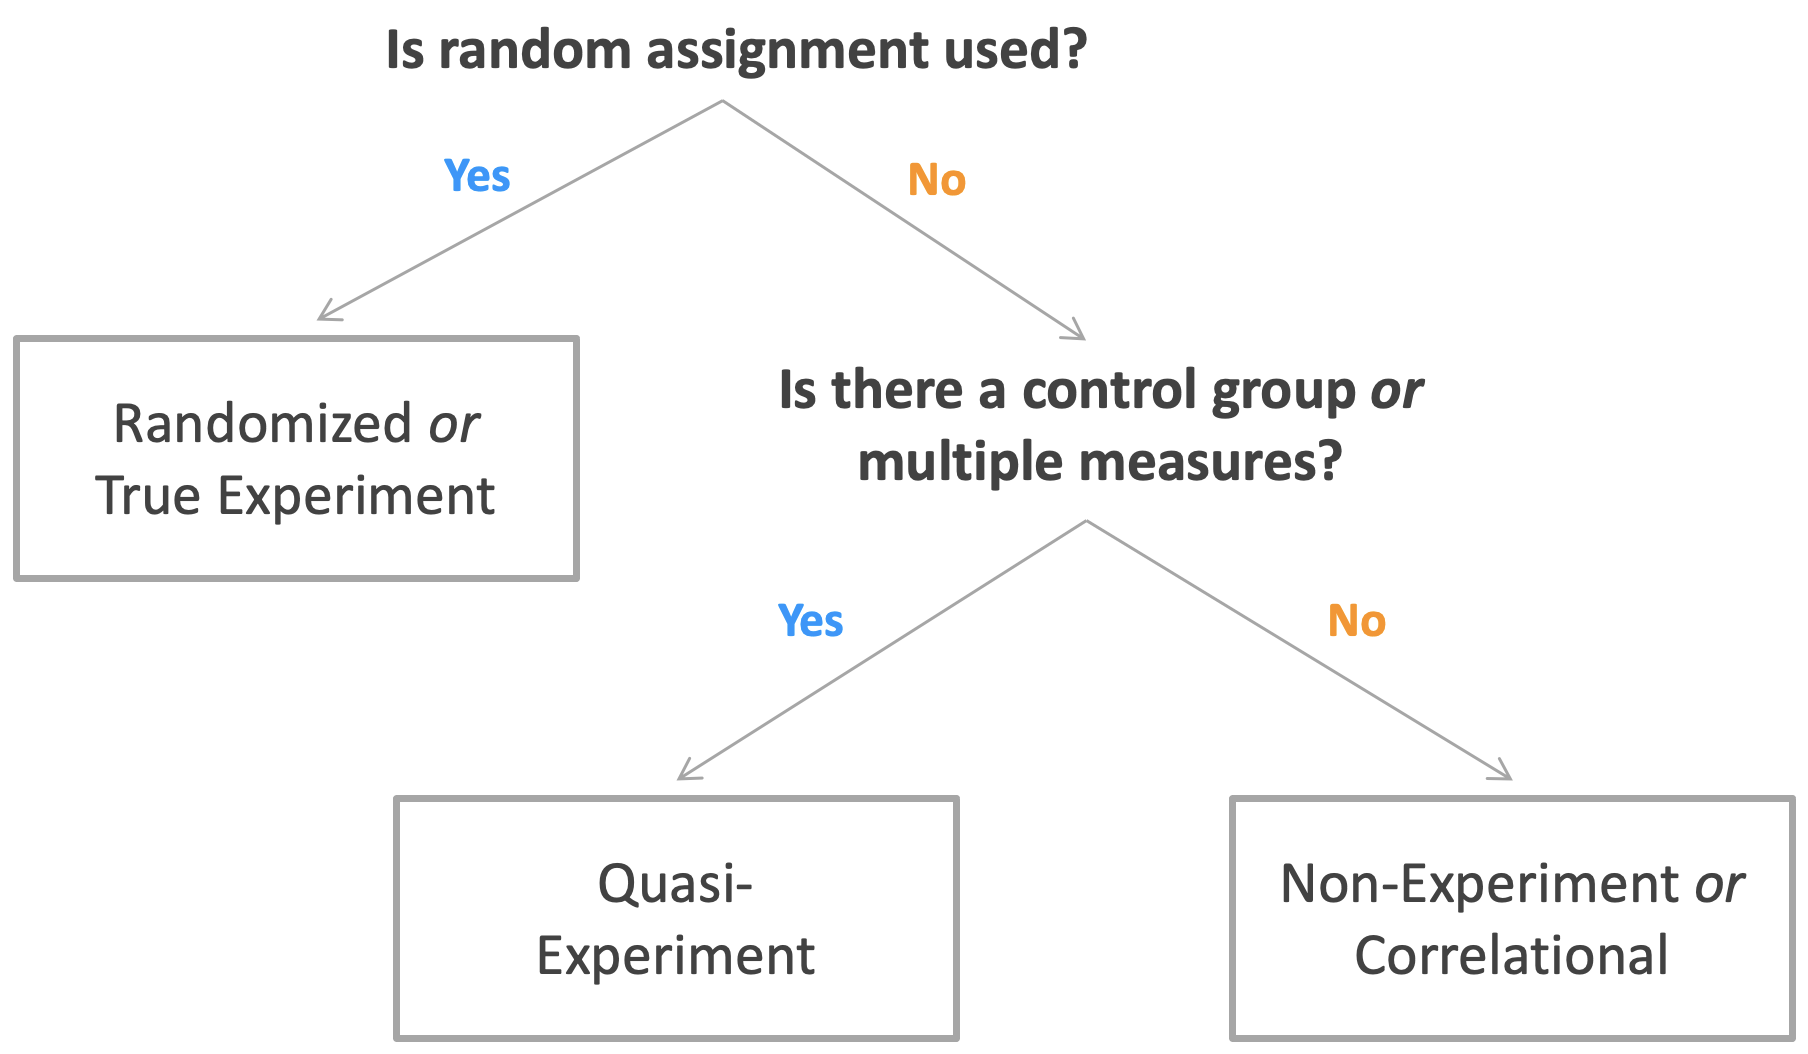
\includegraphics[width=0.75\linewidth]{/Users/craig.starbuck/Library/Mobile Documents/com~apple~CloudDocs/Documents/People Analytics Book/GitHub/peopleanalytics_lifecycle_book/graphics/research_designs} 

}

\caption{Quantitative Research Designs}\label{fig:res-designs}
\end{figure}

\textbf{Experimental Research}

\textbf{Experimental research} is concerned with casual (internal) validity. Randomized experimental designs provide the most rigor with regard to causal validity. However, in social science research contexts, true experiments often are not possible due to ethical considerations.

For example, if we were interested in understanding the causal effect leadership quality has on employee engagement, based on a hypothesis that poor leadership decreases employee engagement, we would need to randomly assign employees to one of two groups that are identical on the basis of all variables that could theoretically explain why employees vary in their levels of engagement. Then, we would need to manipulate the variable of interest (leadership quality) to evaluate if the group of employees subjected to poor leadership (treatment group) reports significantly different levels of engagement relative to the group of employees for whom leadership quality has not been manipulated (control group). In a practical setting, it would of course be unethical to purposefully subject employees to poor leadership with the expectation of reducing engagement -- and consequently, retention, productivity, and impact to the organization.

Clinical trials are a common setting for true experiments, as isolating the effects of an experimental drug can be a matter of life or death. In a randomized clinical trial, patients are randomly assigned to an experimental group (patients who receive the drug) or control group (patients who receive a placebo). To protect against placebo effects biasing the results, patients do not know if they receive the experimental treatment or the placebo. Done correctly, these experiments have the highest level of internal validity.

Another example of an experimental design is \textbf{A/B testing}. A/B testing is often performed in the context of website optimization, in which two or more versions of the site are shown to customers to identify which version impacts key success metrics more positively. In a people analytics context, we may create two versions of a dashboard and \emph{randomly} assign the permissioned users to each. We could then assess whether utilization rates, average usage time, repeat usage, among other success measures are significantly different between the two groups of users to inform which design is most effective.

\textbf{Quasi-Experimental Research}

\textbf{Quasi-experimental research} is an experiment in which participants cannot be randomly assigned.

In the case of our leadership quality example, a quasi-experiment may examine engagement differences between two groups of employees who rate their leader either favorably (Group A) or unfavorably (Group B). A key limitation of this approach is that the groups may be different in important ways beyond leader perception incongruities. For example, Group A employees may be concentrated within a single department, whereas Group B employees may span all other departments. This would indicate that the difference in leadership -- and presumably engagement -- is driven by factors unique to the department, making it more challenging to isolate the effects of leadership quality on engagement. Perhaps the department with unfavorable leader perceptions has seen significant attrition, or the department is largely first-time people leaders in need of coaching and support.

Another example of quasi-experiments is a pretest-posttest setting in which there are multiple measures. Random assignment could be used in pretest-posttest contexts, in which case this would be characterized as a true experiment, but often this approach is implemented without random assignment. For example, we could test the hypothesized effect of leadership quality on engagement via a pretest-posttest approach. If leaders are selected for a leadership development workshop, we could survey the leaders' teams and collect data on leader effectiveness perceptions and self-reported engagement prior to, and after, the workshop. It is unlikely that leaders were selected for this workshop by a random process; more likely, there were criteria driving the selection, such as leaders who were identified as critical talent or who achieved a certain performance level. If this study finds that improvements in leadership effectiveness correlate with improvements in engagement, there would be \emph{some} evidence in favor of improving leadership quality; however, this would not be sufficient evidence for a causal effect.

Though quasi-experiments are not as robust as true experiments, they are usually more feasible in a people analytics context. True experiments control for confounding variables by way of the research design (randomization ensures equivalent groups), while these factors must be controlled statistically in quasi-experimental contexts. In Chapter \ref{lm}, we will discuss how to model relationships among multiple variables (multivariate analysis) in order to study how one variable influences another while holding constant variables that may influence the outcome but are not the primary focus of the research.

\textbf{Non-Experimental Research}

Unlike experimental and quasi-experimental designs, \textbf{non-experimental research} does not involve the manipulation of an IV. The goal of non-experiments is not to provide evidence for causal effects, but to study measured variables as they naturally occur.

Given the potential for alternative explanations of any observed differences or relationships, non-experimental research tends to have lower internal validity than experimental and quasi-experimental designs. As we have discussed, it is often not possible or ethical to manipulate IVs or to randomly assign people to groups. In addition, the nature of research questions does not always warrant experiments. In these cases, one or three non-experimental approaches may be considered: (a) \emph{cross-sectional}, (b) \emph{correlational}, and (c) \emph{observational}.

\textbf{Cross-sectional research} compares two or more natural groups of people. For example, we may examine differences in engagement between employees in the Engineering department relative to employees in the Product department. In this case, we would neither manipulate one's department to determine how department influences engagement, nor randomly assign employees to these departments. Department membership exists apart from the research, so these naturally occurring groups can be leveraged for comparisons. There are of course many examples of naturally occurring groups that we would not manipulate, such as gender, ethnicity, generation, education, job family, job level, location, and tenure band. When participant characteristics are used to create groups, the IV is sometimes referred to as \emph{experimenter-selected} rather than \emph{experimenter-manipulated} IVs.

\textbf{Correlational research} involves studying the statistical relationship between two variables without the manipulation of an IV. The relationship between leadership quality and engagement could be evaluated using correlational research. However, we would be unable to leverage a correlational design to test a hypothesis positing a causal effect of leadership quality on engagement. We would be limited to understanding how leadership quality and engagement covary; that is, to what extent a change in one variable is associated with a change in the other. Engagement may tend to increase as leadership quality increases, but a correlational design does not lend to understanding the direction of causal influence -- if such an effect exists.

\textbf{Observational research} refers to studies in which the researcher gathers information without research subjects being explicitly involved in the recording of data. Collecting data from the company's HRIS could be an observational research method. For example, if we access data on terminations to determine the rate of attrition over a specified period, we would not need to interfere by asking past or present employees for this information. We would also do so without manipulating an IV, tagging people to naturally occurring or artificially created groups, or evaluating the association of attrition with another variable. The reality is that such an approach would not be too actionable, however, as this would offer no understanding of what may be influencing attrition or how attrition varies across departments, jobs, locations, or other theoretically-relevant dimensions.

\hypertarget{exercises-1}{%
\section{Exercises}\label{exercises-1}}

\begin{enumerate}
\def\labelenumi{\arabic{enumi}.}
\item
  What type of research method and design would be best suited for a study aiming to understand the effect of stay interviews on employee attrition?
\item
  Why are quasi-experiments less rigorous than true experiments?
\item
  Why aren't experimental designs always implemented when an experimenter-manipulated IV is warranted?
\item
  What is the role of research questions?
\item
  What is the role of research hypotheses?
\item
  What is the difference between internal and external validity, and why are these concepts important in research?
\item
  What is an example of a mixed methods study?
\item
  What is the key difference between experimental and non-experimental research designs?
\item
  What are the differences between cross-sectional, correlational, and observational non-experimental designs?
\item
  What are some use cases for A/B testing in people analytics?
\end{enumerate}

\hypertarget{uni-bi-stats}{%
\chapter{Univariate \& Bivariate Analysis}\label{uni-bi-stats}}

This chapter reviews essential univariate and bivariate analysis concepts that underpin the more complex multivariate approaches in subsequent chapters of this book.

\hypertarget{univariate-analysis}{%
\section{Univariate Analysis}\label{univariate-analysis}}

\textbf{Descriptive statistics} are rudimentary analysis techniques that help describe and summarize data in a meaningful way. Descriptive statistics do not allow us to draw any conclusions beyond the available data but are helpful in interpreting the data at hand.

There are two categories of descriptive statistics: (a) \textbf{measures of central tendency} describe the central position in a set of data; and (b) \textbf{measures of spread} describe how dispersed the data are.

\hypertarget{measures-of-central-tendency}{%
\subsection{Measures of Central Tendency}\label{measures-of-central-tendency}}

\textbf{Mean}

Perhaps the most intuitive measure of central tendency is the \textbf{mean}, which is often referred to as the average. The mean of a sample is denoted by \(\bar{x}\) and is defined by:

\[ \bar{x} = \frac{\displaystyle\sum_{i=1}^{n} x_{i}}{n} \]

The population mean is denoted by \(\mu\) and is defined by:

\[ \mu = \frac{\displaystyle\sum_{i=1}^{n} x_{i}}{N} \]

The mean of a set of numeric values can be calculated using the mean() function in R:

\begin{Shaded}
\begin{Highlighting}[]
\CommentTok{# Fill vector x with integers}
\NormalTok{x <-}\StringTok{ }\KeywordTok{c}\NormalTok{(}\DecValTok{1}\NormalTok{,}\DecValTok{1}\NormalTok{,}\DecValTok{1}\NormalTok{,}\DecValTok{2}\NormalTok{,}\DecValTok{2}\NormalTok{,}\DecValTok{2}\NormalTok{,}\DecValTok{3}\NormalTok{,}\DecValTok{3}\NormalTok{,}\DecValTok{4}\NormalTok{,}\DecValTok{50}\NormalTok{)}

\CommentTok{# Calculate average of vector x}
\KeywordTok{mean}\NormalTok{(x)}
\end{Highlighting}
\end{Shaded}

\begin{verbatim}
## [1] 6.9
\end{verbatim}

\textbf{Median}

The \textbf{median} represents the midpoint in a sorted vector of numbers. For vectors with an even number of values, the median is the average of the middle two numbers; it is simply the middle number for vectors with an odd number of values. When the distribution of data is skewed, or there is an extreme value like we observe in vector x, the median is a better measure of central tendency.

The median() function in R can be used to handle the sorting and midpoint selection:

\begin{Shaded}
\begin{Highlighting}[]
\CommentTok{# Calculate median of vector x}
\KeywordTok{median}\NormalTok{(x)}
\end{Highlighting}
\end{Shaded}

\begin{verbatim}
## [1] 2
\end{verbatim}

In this example, the median is only 2 while the mean is 6.9 (which is not representative of any of the values in vector \(x\)). Large deltas between mean and median values are evidence of outliers.

\textbf{Mode}

The \textbf{mode} is the most frequent number in a set of values.

While mean() and median() are standard functions in R, mode() returns the internal storage mode of the object rather than the statistical mode of the data. We can easily create a function to return the statistical mode(s):

\begin{Shaded}
\begin{Highlighting}[]
\CommentTok{# Create function to calculate statistical mode(s)}
\NormalTok{stat.mode <-}\StringTok{ }\ControlFlowTok{function}\NormalTok{(x) \{}
\NormalTok{  ux <-}\StringTok{ }\KeywordTok{unique}\NormalTok{(x)}
\NormalTok{  tab <-}\StringTok{ }\KeywordTok{tabulate}\NormalTok{(}\KeywordTok{match}\NormalTok{(x, ux))}
\NormalTok{  ux[tab }\OperatorTok{==}\StringTok{ }\KeywordTok{max}\NormalTok{(tab)]}
\NormalTok{\}}

\CommentTok{# Return mode(s) of vector x}
\KeywordTok{stat.mode}\NormalTok{(x)}
\end{Highlighting}
\end{Shaded}

\begin{verbatim}
## [1] 1 2
\end{verbatim}

In this case, we have a bimodal distribution since both 1 and 2 occur most frequently.

\textbf{Range}

The \textbf{range} is the difference between the maximum and minimum values in a set of numbers.

The range() function in R returns the minimum and maximum numbers:

\begin{Shaded}
\begin{Highlighting}[]
\CommentTok{# Return lowest and highest values of vector x}
\KeywordTok{range}\NormalTok{(x)}
\end{Highlighting}
\end{Shaded}

\begin{verbatim}
## [1]  1 50
\end{verbatim}

We can leverage the max() and min() functions to calculate the difference between these values:

\begin{Shaded}
\begin{Highlighting}[]
\CommentTok{# Calculate range of vector x}
\KeywordTok{max}\NormalTok{(x, }\DataTypeTok{na.rm =} \OtherTok{TRUE}\NormalTok{) }\OperatorTok{-}\StringTok{ }\KeywordTok{min}\NormalTok{(x, }\DataTypeTok{na.rm =} \OtherTok{TRUE}\NormalTok{)}
\end{Highlighting}
\end{Shaded}

\begin{verbatim}
## [1] 49
\end{verbatim}

In people analytics, there are many conventional descriptive metrics -- largely counts, percentages, and ratios cut by time series (day, month, quarter, year) and categorical dimensions (department, job, location, tenure band). Here is a sample of common measures:

\begin{itemize}
\tightlist
\item
  Time to Fill: average days between job requisition posting and offer acceptance
\item
  Offer Acceptance Rate: percent of offers extended to candidates that are accepted
\item
  Pass-Through Rate: percent of candidates in a particular stage of the recruiting process who passed through to the next stage
\item
  Progress to Goal: percent of approved positions that have been filled
\item
  cNPS/eNPS: candidate and employee NPS (-100 to 100)
\item
  Headcount: counts and percent of workforce across worker types (employee, intern, contingent)
\item
  Diversity: counts and percent of workforce across gender, ethnicity, and generational cohorts
\item
  Positions: count and percent of open, committed, and filled seats
\item
  Hires: counts and rates
\item
  Career Moves: counts and rates
\item
  Turnover: counts and rates (usually terms / average headcount over the period)
\item
  Workforce Growth: net changes over time, accounting for hires, internal transfers, and exits
\item
  Span of Control: ratio of people leaders to individual contributors
\item
  Layers/Tiers: average and median number of layers removed from CEO
\item
  Engagement: average score or top-box favorability score
\end{itemize}

\hypertarget{measures-of-spread}{%
\subsection{Measures of Spread}\label{measures-of-spread}}

\textbf{Variance}

\textbf{Variance} is a measure of variability in the data. Variance is calculated using the average of squared differences -- or deviations -- from the mean.

Variance of a population is defined by:

\[ \sigma^{2} = \frac{\displaystyle\sum_{i=1}^{n} (x_{i}-\mu)^{2}}{N} \]

Variance of a sample is defined by:

\[ s^{2} = \frac{\displaystyle\sum_{i=1}^{n} (x_{i}-\bar{x})^{2}}{n-1} \]

It is important to note that since differences are squared, the variance is always non-negative. In addition, we cannot compare these squared differences to the arithmetic mean since the units are different. For example, if we calculate the variance of annual compensation measured in USD, variance should be expressed as USD squared while the mean exists in the original USD unit of measurement.

In R, the sample variance can be calculated using the var() function:

\begin{Shaded}
\begin{Highlighting}[]
\CommentTok{# Load library for data wrangling}
\KeywordTok{library}\NormalTok{(dplyr)}

\CommentTok{# Read employee demographics data}
\NormalTok{demographics <-}\StringTok{ }\KeywordTok{read.csv}\NormalTok{(}\StringTok{"https://raw.githubusercontent.com/crstarbuck/peopleanalytics_lifecycle_book/master/data/files/employee_demographics.csv"}\NormalTok{)}

\CommentTok{# Calculate sample variance for annual compensation}
\KeywordTok{var}\NormalTok{(demographics}\OperatorTok{$}\NormalTok{annual_comp)}
\end{Highlighting}
\end{Shaded}

\begin{verbatim}
## [1] 1876688425
\end{verbatim}

Sample statistics are the default in R. Since the population variance differs from the sample variance by a factor of \(s^2 (\frac{n - 1}{n})\), it is simple to convert output from var() to the population variance:

\begin{Shaded}
\begin{Highlighting}[]
\CommentTok{# Store number of observations}
\NormalTok{n =}\StringTok{ }\KeywordTok{length}\NormalTok{(demographics}\OperatorTok{$}\NormalTok{annual_comp)}

\CommentTok{# Calculate population variance for annual compensation}
\KeywordTok{var}\NormalTok{(demographics}\OperatorTok{$}\NormalTok{annual_comp) }\OperatorTok{*}\StringTok{ }\NormalTok{(n }\OperatorTok{-}\StringTok{ }\DecValTok{1}\NormalTok{) }\OperatorTok{/}\StringTok{ }\NormalTok{n}
\end{Highlighting}
\end{Shaded}

\begin{verbatim}
## [1] 1876303464
\end{verbatim}

\textbf{Standard Deviation}

The \textbf{standard deviation} is simply the square root of the variance.

The standard deviation of a population is defined by:

\[ \sigma = \sqrt{\frac{\displaystyle\sum_{i=1}^{n} (x_{i} - \mu)^{2}}{N}} \]

The standard deviation of a sample is defined by:

\[ s = \sqrt{\frac{\displaystyle\sum_{i=1}^{n} (x_{i} - \bar{x})^{2}}{n - 1}} \]

Since a squared value can be converted back to its original units by taking its square root, the standard deviation expresses variability around the mean in the variable's original units.

In R, the sample standard deviation can be calculated using the sd() function:

\begin{Shaded}
\begin{Highlighting}[]
\CommentTok{# Calculate sample standard deviation for annual compensation}
\KeywordTok{sd}\NormalTok{(demographics}\OperatorTok{$}\NormalTok{annual_comp)}
\end{Highlighting}
\end{Shaded}

\begin{verbatim}
## [1] 43320.76
\end{verbatim}

Since the population standard deviation differs from the sample standard deviation by a factor of \(s \sqrt \frac{n - 1}{n}\), it is simple to convert output from sd() to the population standard deviation:

\begin{Shaded}
\begin{Highlighting}[]
\CommentTok{# Calculate population standard deviation for annual compensation}
\KeywordTok{sd}\NormalTok{(demographics}\OperatorTok{$}\NormalTok{annual_comp) }\OperatorTok{*}\StringTok{ }\KeywordTok{sqrt}\NormalTok{((n }\OperatorTok{-}\StringTok{ }\DecValTok{1}\NormalTok{) }\OperatorTok{/}\StringTok{ }\NormalTok{n)}
\end{Highlighting}
\end{Shaded}

\begin{verbatim}
## [1] 43316.32
\end{verbatim}

\textbf{Quartiles}

\textbf{Quartiles} are a staple of exploratory data analysis (EDA). A quartile is a type of quantile that partitions data into four equally sized parts after ordering the data. Note that each partition is equally sized with respect to the number of data points -- not the range of values in each. Quartiles are also related to \textbf{percentiles}. For example, Q1 is the 25th percentile -- the value at or below which 25\% of values lie. Percentiles are likely more familiar than quartiles, as percentiles show up in the height and weight measurements of babies, performance on standardized tests like the SAT and GRE, among other things.

The \textbf{Interquartile Range (IQR)} represents the difference between Q3 and Q1 cut point values (the middle two quartiles). The IQR is sometimes used to detect extreme values in a distribution; values less than \(Q1 - 1.5 * IQR\) or greater than \(Q3 + 1.5 * IQR\) are generally considered outliers.

In R, the quantile() function returns the values that bookend each quartile:

\begin{Shaded}
\begin{Highlighting}[]
\CommentTok{# Return quartiles for annual compensation}
\KeywordTok{quantile}\NormalTok{(demographics}\OperatorTok{$}\NormalTok{annual_comp)}
\end{Highlighting}
\end{Shaded}

\begin{verbatim}
##       0%      25%      50%      75%     100% 
##  50016.0  87946.0 125522.0 163262.5 199968.0
\end{verbatim}

Based on this output, we know that 25\% of people in our data earn annual compensation of 87,946 USD or less, 125,522 USD is the median annual compensation, and 75\% of people earn annual compensation of 163,263 USD or less.

\textbf{Boxplots} are a common way to visualize the distribution of data by categorical and ordinal factors. Boxplots are not usually found in presentations to stakeholders, since they are a bit more technical and often require explanation, but these are very useful to analysts for understanding data distributions during the EDA phase. In R, the \texttt{ggplot2} library has robust and flexible data visualization capabilities which we will leverage throughout this book. Let's visualize the spread of annual compensation by education level and gender using the ggplot() function:

\begin{Shaded}
\begin{Highlighting}[]
\CommentTok{# Load library for data viz}
\KeywordTok{library}\NormalTok{(ggplot2)}
\end{Highlighting}
\end{Shaded}

\begin{verbatim}
## Warning: package 'ggplot2' was built under R version 4.0.2
\end{verbatim}

\begin{Shaded}
\begin{Highlighting}[]
\CommentTok{# Produce boxplots to visualize compensation distribution by education and gender}
\KeywordTok{ggplot}\NormalTok{(demographics, }\KeywordTok{aes}\NormalTok{(}\DataTypeTok{x =} \KeywordTok{as.factor}\NormalTok{(education), }\DataTypeTok{y =}\NormalTok{ annual_comp, }\DataTypeTok{color =}\NormalTok{ gender)) }\OperatorTok{+}
\StringTok{  }\KeywordTok{labs}\NormalTok{(}\DataTypeTok{x =} \StringTok{"Education"}\NormalTok{, }\DataTypeTok{y =} \StringTok{"Annual Compensation"}\NormalTok{) }\OperatorTok{+}\StringTok{ }
\StringTok{  }\KeywordTok{theme_bw}\NormalTok{() }\OperatorTok{+}
\StringTok{  }\KeywordTok{geom_boxplot}\NormalTok{()}
\end{Highlighting}
\end{Shaded}

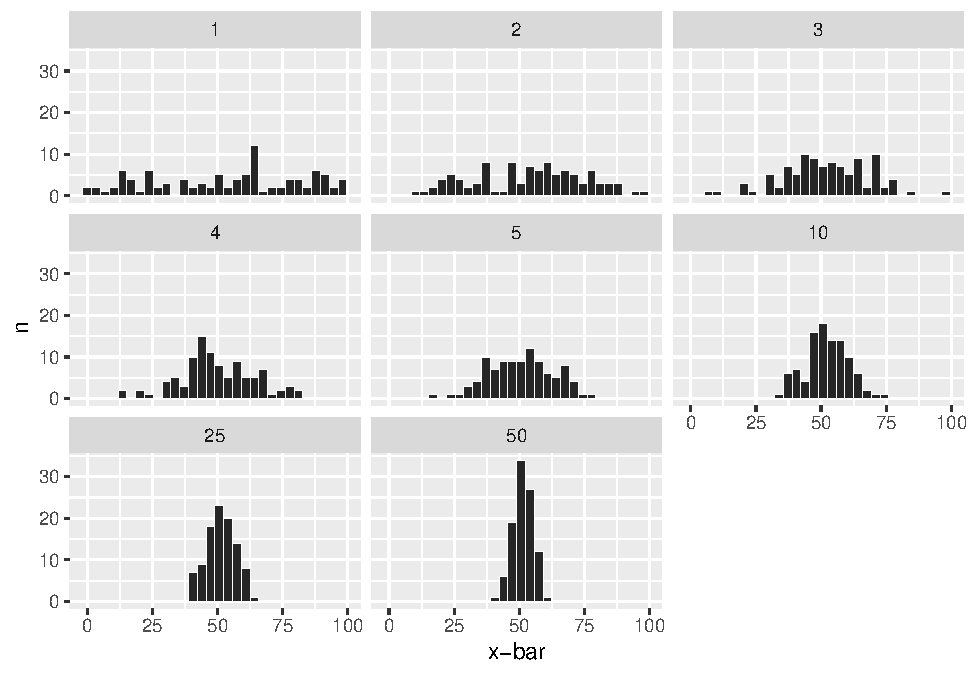
\includegraphics{People_Analytics_Lifecycle_files/figure-latex/unnamed-chunk-39-1.pdf}

Boxplots can be interpreted as follows:
* Horizontal lines represent median compensation values.
* The box in the middle of each distribution represents the IQR.
* The end of the line above the IQR represents the threshold for outliers in the upper range: \(Q3 + 1.5 * IQR\).
* The end of the line below the IQR represents the threshold for outliers in the lower range: \(Q1 - 1.5 * IQR\).
* Data points represent outliers: \(x > Q3 + 1.5 * IQR\) or \(x < Q1 - 1.5 * IQR\).

We can also return a specific percentile value using the \texttt{probs} argument in the quantile() function. For example, if we want to know the 80th percentile annual compensation value, we can execute the following:

\begin{Shaded}
\begin{Highlighting}[]
\CommentTok{# Return 80th percentile annual compensation value}
\KeywordTok{quantile}\NormalTok{(demographics}\OperatorTok{$}\NormalTok{annual_comp, }\DataTypeTok{probs =} \FloatTok{.8}\NormalTok{)}
\end{Highlighting}
\end{Shaded}

\begin{verbatim}
##      80% 
## 170196.4
\end{verbatim}

In addition, the summary() function returns several common descriptive statistics for an object:

\begin{Shaded}
\begin{Highlighting}[]
\CommentTok{# Return common descriptives}
\KeywordTok{summary}\NormalTok{(demographics}\OperatorTok{$}\NormalTok{annual_comp)}
\end{Highlighting}
\end{Shaded}

\begin{verbatim}
##    Min. 1st Qu.  Median    Mean 3rd Qu.    Max. 
##   50016   87946  125522  125369  163262  199968
\end{verbatim}

\textbf{Skewness}

\textbf{Skewness} is a measure of the horizontal distance between the mode and mean -- a representation of symmetric distortion. In most practical settings, data are not normally distributed. That is, the data are skewed either positively (right-tailed distribution) or negatively (left-tailed distribution). The coefficient of skewness is one of many ways in which we can asertain the degree of skew in the data. The skewness of sample data is defined as:

\[ Sk = \frac{1}{n} \frac{\displaystyle\sum_{i=1}^{n} (x_i-\bar{x})^3}{s^3} \]

A positive skewness coefficient indicates positive skew, while a negative coefficient indicates negative skew. The order of descriptive statistics can also be leveraged to ascertain the direction of skew in the data:

\begin{itemize}
\tightlist
\item
  Positive skewness: mode \textless{} median \textless{} mean
\item
  Negative skewness: mode \textgreater{} median \textgreater{} mean
\item
  Symmetrical distribution: mode = median = mean
\end{itemize}

Figure \ref{fig:skewness} illustrates the placement of these descriptive statistics in each of the three types of distributions:

\begin{figure}

{\centering 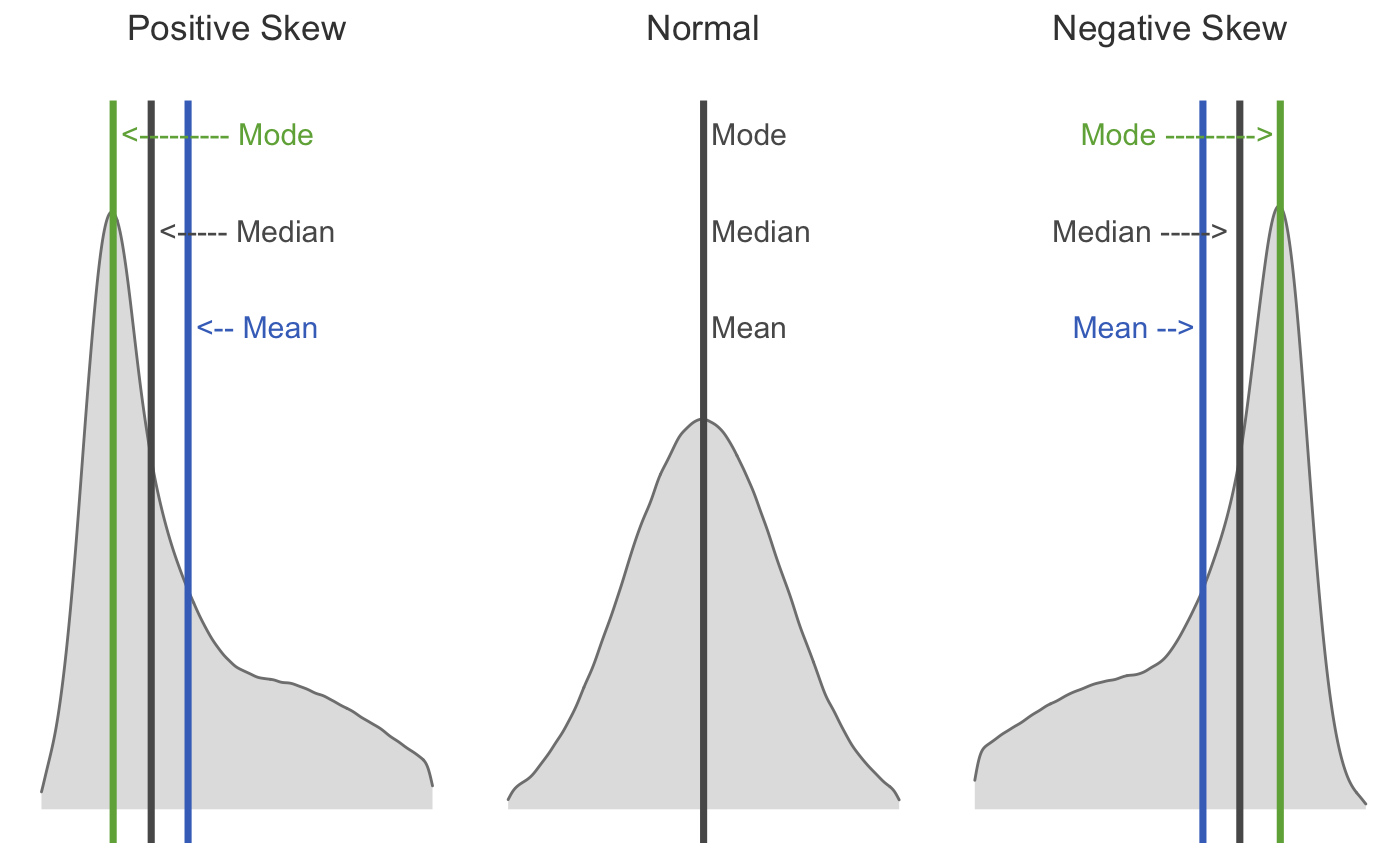
\includegraphics[width=1\linewidth]{/Users/craig.starbuck/Library/Mobile Documents/com~apple~CloudDocs/Documents/People Analytics Book/GitHub/peopleanalytics_lifecycle_book/graphics/skewness} 

}

\caption{Skewness}\label{fig:skewness}
\end{figure}

The magnitude of skewness can be determined by measuring the distance between the mode and mean relative to the variable's scale. Alternatively, we can simply evaluate this using the coefficient of skewness:

\begin{itemize}
\tightlist
\item
  If skewness is between -0.5 - 0.5, the data are symmetrical.
\item
  If skewness is between -0.5 and -1 or 0.5 and 1, the data are moderately skewed.
\item
  If skewness is \textless{} -1 or \textgreater{} 1, the data are highly skewed.
\end{itemize}

Since there is not a base R function for skewness, we can leverage the moments library to calculate skewness:

\begin{Shaded}
\begin{Highlighting}[]
\CommentTok{# Load library}
\KeywordTok{library}\NormalTok{(moments)}

\CommentTok{# Calculate skewness for org tenure, rounded to three significant figures}
\KeywordTok{round}\NormalTok{(}\KeywordTok{skewness}\NormalTok{(demographics}\OperatorTok{$}\NormalTok{org_tenure), }\DecValTok{3}\NormalTok{)}
\end{Highlighting}
\end{Shaded}

\begin{verbatim}
## [1] 0.562
\end{verbatim}

\textbf{Statistical Moments}, after which this library was named, play an important role in specifying the appropriate probability distribution for a set of data. Moments are a set of statistical parameters used to describe the characteristics of a distribution. Skewness is the third statistical moment in the set; hence the sum of cubed differences and cubic polynomial in the denominator of the formula above. The complete set of moments comprises: (1) expected value or mean, (2) variance and standard deviation, (3) skewness, and (4) kurtosis.

We can verify that the skewness() function from the moments library returns the expected value (per the aforementioned formula) by validating against a manual calculation:

\begin{Shaded}
\begin{Highlighting}[]
\CommentTok{# Store components of skewness calculation}
\NormalTok{n =}\StringTok{ }\KeywordTok{length}\NormalTok{(demographics}\OperatorTok{$}\NormalTok{org_tenure)}
\NormalTok{x =}\StringTok{ }\NormalTok{demographics}\OperatorTok{$}\NormalTok{org_tenure}
\NormalTok{x_bar =}\StringTok{ }\KeywordTok{mean}\NormalTok{(demographics}\OperatorTok{$}\NormalTok{org_tenure)}
\NormalTok{s =}\StringTok{ }\KeywordTok{sd}\NormalTok{(demographics}\OperatorTok{$}\NormalTok{org_tenure)}

\CommentTok{# Calculate skewness manually, rounded to three significant figures}
\KeywordTok{round}\NormalTok{(}\DecValTok{1}\OperatorTok{/}\NormalTok{n }\OperatorTok{*}\StringTok{ }\NormalTok{(}\KeywordTok{sum}\NormalTok{((x }\OperatorTok{-}\StringTok{ }\NormalTok{x_bar)}\OperatorTok{^}\DecValTok{3}\NormalTok{) }\OperatorTok{/}\StringTok{ }\NormalTok{s}\OperatorTok{^}\DecValTok{3}\NormalTok{), }\DecValTok{3}\NormalTok{)}
\end{Highlighting}
\end{Shaded}

\begin{verbatim}
## [1] 0.562
\end{verbatim}

A skewness coefficient of .562 indicates that organization tenure is moderately and positively skewed. We can visualize the data to confirm the expected right-tailed distribution:

\begin{Shaded}
\begin{Highlighting}[]
\CommentTok{# Produce histogram to visualize sample distribution}
\KeywordTok{ggplot}\NormalTok{() }\OperatorTok{+}\StringTok{ }
\StringTok{  }\KeywordTok{aes}\NormalTok{(demographics}\OperatorTok{$}\NormalTok{org_tenure) }\OperatorTok{+}\StringTok{ }
\StringTok{  }\KeywordTok{labs}\NormalTok{(}\DataTypeTok{x =} \StringTok{"Organization Tenure"}\NormalTok{, }\DataTypeTok{y =} \StringTok{"Density"}\NormalTok{) }\OperatorTok{+}\StringTok{ }
\StringTok{  }\KeywordTok{geom_histogram}\NormalTok{(}\KeywordTok{aes}\NormalTok{(}\DataTypeTok{y =}\NormalTok{ ..density..), }\DataTypeTok{fill =} \StringTok{"#414141"}\NormalTok{) }\OperatorTok{+}
\StringTok{  }\KeywordTok{geom_density}\NormalTok{(}\DataTypeTok{fill =} \StringTok{"#ADD8E6"}\NormalTok{, }\DataTypeTok{alpha =} \FloatTok{0.6}\NormalTok{) }\OperatorTok{+}
\StringTok{  }\KeywordTok{theme_bw}\NormalTok{()}
\end{Highlighting}
\end{Shaded}

\begin{figure}

{\centering 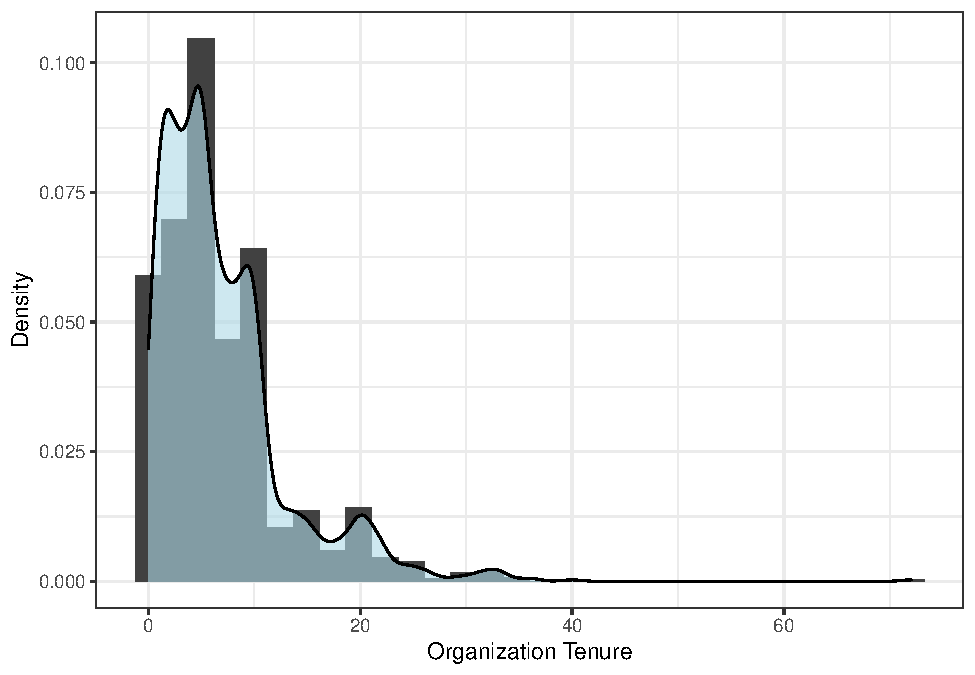
\includegraphics{People_Analytics_Lifecycle_files/figure-latex/org-tenure-distribution-1} 

}

\caption{Organization Tenure Distribution}\label{fig:org-tenure-distribution}
\end{figure}

\textbf{Kurtosis}

While skewness provides information on the symmetry of a distribution, \textbf{kurtosis} provides information on the heaviness of a distribution's tails (``tailedness''). Kurtosis is the fourth statistical moment, defined by:

\[ K = \frac{1}{n} \frac{\displaystyle\sum_{i=1}^{n} (x_i-\bar{x})^4}{s^4} \]

Note that the quartic functions characteristic of the fourth statistical moment are the only differences from the skewness formula we reviewed in the prior section (which featured cubic functions).

The terms \textbf{leptokurtic} and \textbf{platykurtic} are often used to describe distributions with light and heavy tails, respectively. ``Platy-'' in platykurtic is the same root as ``platypus'', and I've found it helpful to recall the characteristics of the flat platypus when characterizing frequency distributions as platkurtic (wide and flat) vs.~its antithesis, leptokurtic (tall and skinny). The normal (or Gaussian) distribution is referred to as a \textbf{mesokurtic} distribution in the context of kurtosis.

Figure \ref{fig:kurtosis} illustrates the three kurtosis categorizations:

\begin{figure}

{\centering 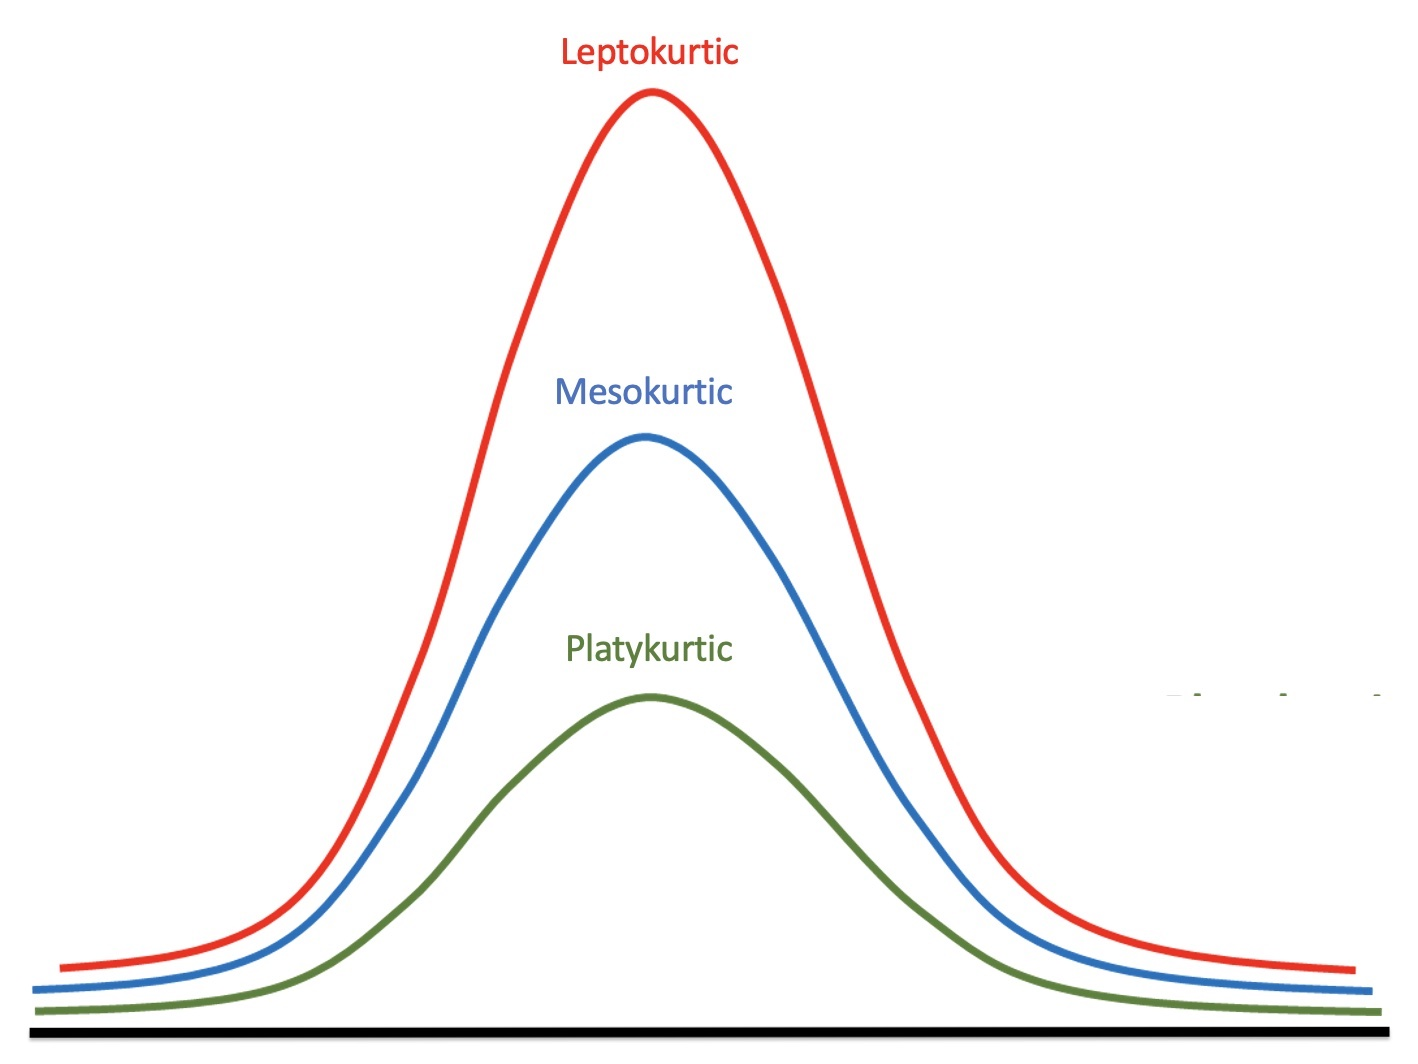
\includegraphics[width=0.75\linewidth]{/Users/craig.starbuck/Library/Mobile Documents/com~apple~CloudDocs/Documents/People Analytics Book/GitHub/peopleanalytics_lifecycle_book/graphics/kurtosis} 

}

\caption{Kurtosis}\label{fig:kurtosis}
\end{figure}

Kurtosis is measured relative to a normal distribution. Normal distributions have a kurtosis coefficient of 3. Therefore, the kurtosis coefficient is greater than 3 for leptokurtic distributions and less than 3 for platykurtic distributions.

The moments library can also be used to calculate kurtosis in R:

\begin{Shaded}
\begin{Highlighting}[]
\CommentTok{# Calculate kurtosis for org tenure, rounded to two significant figures}
\KeywordTok{round}\NormalTok{(}\KeywordTok{kurtosis}\NormalTok{(demographics}\OperatorTok{$}\NormalTok{org_tenure), }\DecValTok{2}\NormalTok{)}
\end{Highlighting}
\end{Shaded}

\begin{verbatim}
## [1] 2.26
\end{verbatim}

We can verify that the kurtosis() function returns the expected value (per the aforementioned formula) by validating against a manual calculation:

\begin{Shaded}
\begin{Highlighting}[]
\CommentTok{# Calculate kurtosis manually, rounded to two significant figures}
\KeywordTok{round}\NormalTok{(}\DecValTok{1}\OperatorTok{/}\NormalTok{n }\OperatorTok{*}\StringTok{ }\NormalTok{(}\KeywordTok{sum}\NormalTok{((x }\OperatorTok{-}\StringTok{ }\NormalTok{x_bar)}\OperatorTok{^}\DecValTok{4}\NormalTok{) }\OperatorTok{/}\StringTok{ }\NormalTok{s}\OperatorTok{^}\DecValTok{4}\NormalTok{), }\DecValTok{2}\NormalTok{)}
\end{Highlighting}
\end{Shaded}

\begin{verbatim}
## [1] 2.26
\end{verbatim}

As we saw in Figure \ref{fig:org-tenure-distribution}, there is a long right tail about the organization tenure distribution. However, due to the moderate skew, there is no left tail. Therefore, our kurtosis coefficient is \textless{} 3 since the presence of the right tail is offset by the lack of a left tail. This is why it is important not to characterize a distribution based on a single isolated metric; we need the complete set of statistical moments to fully understand the distribution of data.

\hypertarget{bivariate-analysis}{%
\section{Bivariate Analysis}\label{bivariate-analysis}}

\hypertarget{covariance}{%
\subsection{Covariance}\label{covariance}}

While variance provides an understanding of how values for a single variable vary, \textbf{covariance} is an unstandardized measure of how two variables vary together. Values can range from \(-\infty\) to \(+\infty\), and these values can be used to understand the direction of the linear relationship between variables. Positive covariance values indicate that the variables vary in the same direction (e.g., tend to increase or decrease together), while negative covariance values indicate that the variables vary in opposite directions (e.g., when one increases, the other decreases, or vice versa).

Covariance of a sample is defined by:

\[ cov_{x,y} = \frac{\displaystyle\sum_{i=1}^{n} (x_{i}-\bar{x})(y_{i}-\bar{y})}{n-1} \]

It's important to note that while covariance aids our understanding of the direction of the relationship between two variables, we cannot use it to understand the strength of the association since it is unstandardized. Due to differences in variables' units of measurement, the strength of the relationship between two variables with large covariance could be weak, while the strength of the relationship between another pair of variables with small covariance could be strong.

In R, we can compute the covariance between a pair of numeric variables by passing the two vectors into the cov() function:

\begin{Shaded}
\begin{Highlighting}[]
\CommentTok{# Calculate sample covariance between annual compensation and age using complete observations (missing values will cause issues if not addressed)}
\KeywordTok{cov}\NormalTok{(demographics}\OperatorTok{$}\NormalTok{annual_comp, demographics}\OperatorTok{$}\NormalTok{age, }\DataTypeTok{use =} \StringTok{"complete.obs"}\NormalTok{)}
\end{Highlighting}
\end{Shaded}

\begin{verbatim}
## [1] 453179.1
\end{verbatim}

In this example, using the default Pearson method, the covariance between annual compensation and age is 453179.1. The positive value indicates that annual compensation is generally higher for older employees and lower for younger employees.

Just as we multiplied the sample variance by \((n - 1) / n\) to obtain the population variance, we can apply the same approach to convert the sample covariance returned by cov() to the population covariance:

\begin{Shaded}
\begin{Highlighting}[]
\CommentTok{# Calculate population covariance between annual compensation and age}
\KeywordTok{cov}\NormalTok{(demographics}\OperatorTok{$}\NormalTok{annual_comp, demographics}\OperatorTok{$}\NormalTok{age, }\DataTypeTok{use =} \StringTok{"complete.obs"}\NormalTok{) }\OperatorTok{*}\StringTok{ }\NormalTok{(n }\OperatorTok{-}\StringTok{ }\DecValTok{1}\NormalTok{) }\OperatorTok{/}\StringTok{ }\NormalTok{n}
\end{Highlighting}
\end{Shaded}

\begin{verbatim}
## [1] 453086.1
\end{verbatim}

The examples thus far have only examined associations between two variables at a time. However, rather than looking at isolated pairwise relationships, we can produce a covariance matrix to surface associations among many variables by passing a dataframe or matrix object into the cov() function:

\begin{Shaded}
\begin{Highlighting}[]
\CommentTok{# Generate a correlation matrix among continuous variables}
\KeywordTok{cov}\NormalTok{(demographics[, }\KeywordTok{c}\NormalTok{(}\StringTok{"annual_comp"}\NormalTok{, }\StringTok{"age"}\NormalTok{, }\StringTok{"org_tenure"}\NormalTok{, }\StringTok{"job_tenure"}\NormalTok{)], }\DataTypeTok{use =} \StringTok{"complete.obs"}\NormalTok{)}
\end{Highlighting}
\end{Shaded}

\begin{verbatim}
##              annual_comp          age   org_tenure  job_tenure
## annual_comp 1.876688e+09 453179.07281 138551.67644 61576.73603
## age         4.531791e+05    168.38661     41.56006    17.96902
## org_tenure  1.385517e+05     41.56006     26.03270    11.04572
## job_tenure  6.157674e+04     17.96902     11.04572    13.29996
\end{verbatim}

Using the default Pearson method, the cov() function will return sample variances for each variable down the diagonal, since covariance is not applicable in the context of a variable with itself. We can confirm by producing the variance for age:

\begin{Shaded}
\begin{Highlighting}[]
\CommentTok{# Return sample variance for age}
\KeywordTok{var}\NormalTok{(demographics}\OperatorTok{$}\NormalTok{age)}
\end{Highlighting}
\end{Shaded}

\begin{verbatim}
## [1] 168.3866
\end{verbatim}

As expected, the variance for age (\(s^{2} = 168.39\)) matches the value found in the age x age cell of the covariance matrix.

\hypertarget{correlation}{%
\subsection{Correlation}\label{correlation}}

\textbf{Correlation} is a scaled form of covariance. While covariance provides an unstandardized measure of the direction of a relationship between variables, correlation provides a standardized measure that can be used to quantify both the direction and strength of bivariate relationships. Correlation coefficients range from -1 to 1, where -1 indicates a perfectly negative association, 1 indicates a perfectly positive association, and 0 indicates the absence of an association. \textbf{Pearson's product-moment correlation coefficient} \(r\) is defined by:

\[ r_{x,y} = \frac{\displaystyle\sum_{i=1}^{n} (x_{i}-\bar{x})(y_{i}-\bar{y})}{\sqrt{\displaystyle\sum_{i=1}^{n} (x_{i}-\bar{x})^2 \displaystyle\sum_{i=1}^{n} (y_{i}-\bar{y})^2}} \]

In R, Pearson's \(r\) can be calculated using the cor() function:

\begin{Shaded}
\begin{Highlighting}[]
\CommentTok{# Calculate the correlation between annual compensation and age}
\KeywordTok{cor}\NormalTok{(demographics}\OperatorTok{$}\NormalTok{annual_comp, demographics}\OperatorTok{$}\NormalTok{age, }\DataTypeTok{use =} \StringTok{"complete.obs"}\NormalTok{)}
\end{Highlighting}
\end{Shaded}

\begin{verbatim}
## [1] 0.8061577
\end{verbatim}

While we already know that the relationship between annual compensation and age is positive based on the positive covariance coefficient, Pearson's \(r\) of .81 indicates that the strength of the positive association is strong (\(r\) = 1 is perfectly positive). Though there are no absolute rules for categorizing the strength of relationships, as thresholds often vary by domain, the following is a general rule of thumb for interpreting the strength of bivariate associations:

\begin{itemize}
\tightlist
\item
  Weak = Absolute value of correlation coefficients between 0 and .3
\item
  Moderate = Absolute value of correlation coefficients between .4 and .6
\item
  Strong = Absolute value of correlation coefficients between .7 and 1
\end{itemize}

There are several correlation coefficients, and the measurement scale of \(x\) and \(y\) determine the appropriate type:

\begin{figure}

{\centering 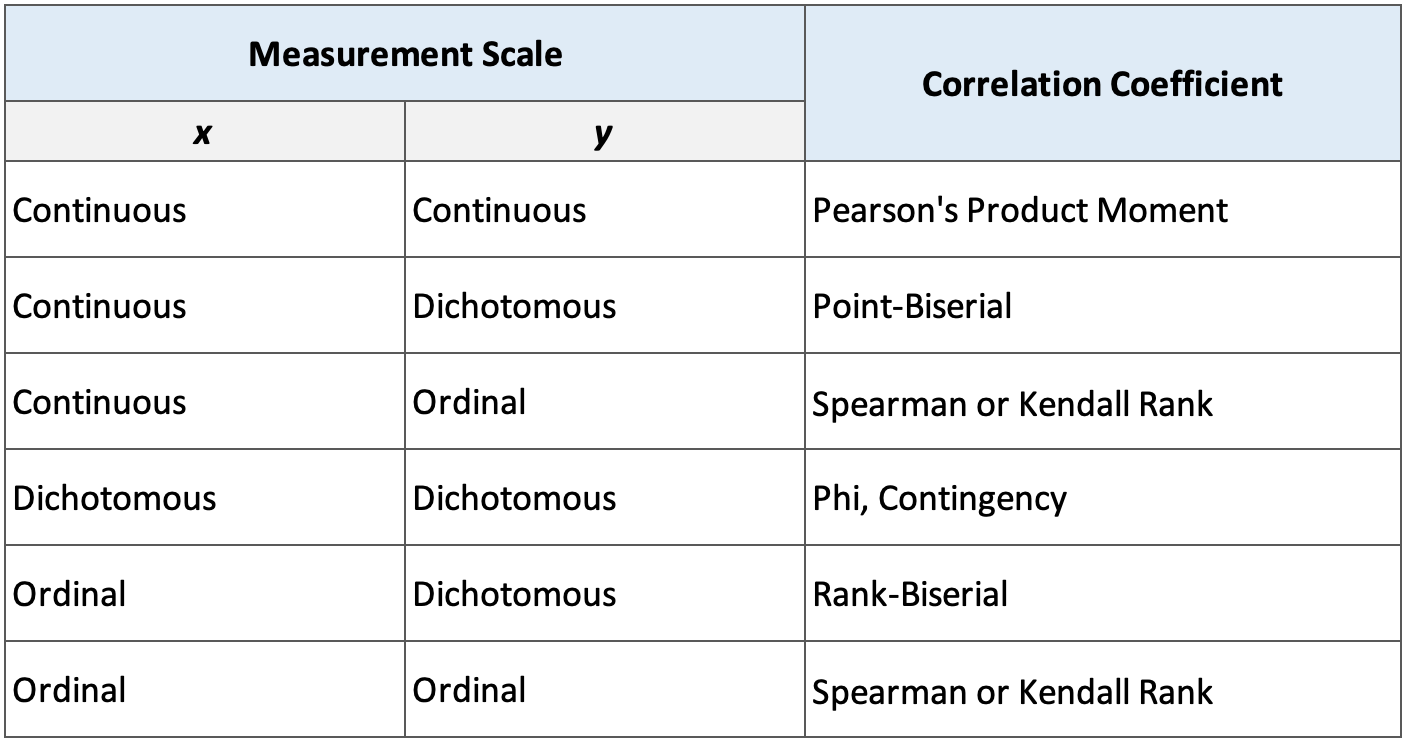
\includegraphics[width=0.75\linewidth]{/Users/craig.starbuck/Library/Mobile Documents/com~apple~CloudDocs/Documents/People Analytics Book/GitHub/peopleanalytics_lifecycle_book/graphics/correlation_table} 

}

\caption{Proper Applications of Correlation Coefficients}\label{fig:corr-table}
\end{figure}

Pearson's \(r\) can be used when both variables are measured on continuous scales or when one is continuous and the other is dichotomous (point-biserial correlation).

When one or both variables are ordinal, we can leverage \textbf{Spearman's} \(\rho\) or \textbf{Kendall's} \(\tau\), which are both standardized nonparametric measures of the association between one or two rank-ordered variables. Let's look at Spearman's \(\rho\), which is defined as:

\[ \rho = 1 - {\frac {6 \sum d_i^2}{n(n^2 - 1)}} \]

We can override the default Pearson method in the cor() function to implement a specific form of rank correlation using the \texttt{method} argument:

\begin{Shaded}
\begin{Highlighting}[]
\CommentTok{# Calculate the correlation between job level and education level using Spearman's method}
\KeywordTok{cor}\NormalTok{(demographics}\OperatorTok{$}\NormalTok{job_level, demographics}\OperatorTok{$}\NormalTok{education, }\DataTypeTok{method =} \StringTok{"spearman"}\NormalTok{, }\DataTypeTok{use =} \StringTok{"complete.obs"}\NormalTok{)}
\end{Highlighting}
\end{Shaded}

\begin{verbatim}
## [1] 0.6749776
\end{verbatim}

The \(\rho\) coefficient of .67 indicates that the positive association we observed between job level and education level is moderate-to-strong. We could also pass \texttt{method\ =\ "kendall"} to this cor() function to implement Kendall's \(\tau\).

The \textbf{Phi Coefficient} (\(\phi\)), sometimes referred to as the mean square contingency coefficient or Matthews correlation in ML, can be used to understand the association between two dichotomous variables. For a 2x2 table for two random variables \(x\) and \(y\):

\begin{figure}

{\centering 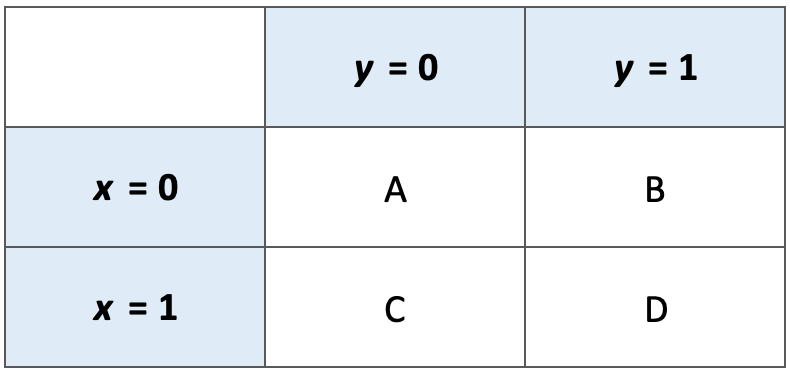
\includegraphics[width=0.5\linewidth]{/Users/craig.starbuck/Library/Mobile Documents/com~apple~CloudDocs/Documents/People Analytics Book/GitHub/peopleanalytics_lifecycle_book/graphics/phi_coefficient_formula} 

}

\caption{2x2 Table for Random Variables x and y}\label{fig:phi-tbl}
\end{figure}

The \(\phi\) coefficient is defined as:

\[ \phi = {\frac {(AD-BC)}{\sqrt{(A+B)(C+D)(A+C)(B+D)}}} \]

To illustrate, let's examine whether there is a relationship between gender and performance after transforming performance from its ordinal form to a dichotomous variable (high vs.~low performance). We can leverage the \texttt{psych} library to calculate \(\phi\) in R:

\begin{Shaded}
\begin{Highlighting}[]
\CommentTok{# Load library for Phi Coefficient}
\KeywordTok{library}\NormalTok{(psych)}

\CommentTok{# Set females to 1 and everything else to 0}
\NormalTok{demographics}\OperatorTok{$}\NormalTok{gender_code <-}\StringTok{ }\KeywordTok{ifelse}\NormalTok{(demographics}\OperatorTok{$}\NormalTok{gender }\OperatorTok{==}\StringTok{ 'Female'}\NormalTok{, }\DecValTok{1}\NormalTok{, }\DecValTok{0}\NormalTok{)}

\CommentTok{# Set high performers (3 and above) to 1 and everything else to 0}
\NormalTok{demographics}\OperatorTok{$}\NormalTok{performance_code <-}\StringTok{ }\KeywordTok{ifelse}\NormalTok{(demographics}\OperatorTok{$}\NormalTok{performance }\OperatorTok{<}\StringTok{ }\DecValTok{3}\NormalTok{, }\DecValTok{0}\NormalTok{, }\DecValTok{1}\NormalTok{)}

\CommentTok{# Create a 2x2 contingency table}
\NormalTok{contingency_tbl <-}\StringTok{ }\KeywordTok{table}\NormalTok{(demographics}\OperatorTok{$}\NormalTok{gender_code, demographics}\OperatorTok{$}\NormalTok{performance_code)}

\CommentTok{# Calculate the Phi Coefficient between dichotomous variables}
\KeywordTok{phi}\NormalTok{(contingency_tbl)}
\end{Highlighting}
\end{Shaded}

\begin{verbatim}
## [1] 0.01
\end{verbatim}

\(\phi\) is essentially 0, which means performance ratings are distributed equitably across gender categories (good news!).

A correlation matrix can be produced to surface associations among many variables by passing a dataframe or matrix object into the cor() function:

\begin{Shaded}
\begin{Highlighting}[]
\CommentTok{# Generate a correlation matrix among continuous variables}
\KeywordTok{cor}\NormalTok{(demographics[, }\KeywordTok{c}\NormalTok{(}\StringTok{"annual_comp"}\NormalTok{, }\StringTok{"age"}\NormalTok{, }\StringTok{"org_tenure"}\NormalTok{, }\StringTok{"job_tenure"}\NormalTok{)], }\DataTypeTok{use =} \StringTok{"complete.obs"}\NormalTok{)}
\end{Highlighting}
\end{Shaded}

\begin{verbatim}
##             annual_comp       age org_tenure job_tenure
## annual_comp   1.0000000 0.8061577  0.6268392  0.3897584
## age           0.8061577 1.0000000  0.6277154  0.3797042
## org_tenure    0.6268392 0.6277154  1.0000000  0.5936211
## job_tenure    0.3897584 0.3797042  0.5936211  1.0000000
\end{verbatim}

Based on this correlation matrix, there are several moderate and strong pairwise associations in the data. The values down the diagonal are 1 because these represent the correlation between each variable and itself. You may also notice that the information above and below the diagonal is identical and, therefore, redundant.

A great R library for visualizing correlation matrices is corrplot. Several arguments can be specified for various visual representations of the relationships among variables:

\begin{Shaded}
\begin{Highlighting}[]
\CommentTok{# Load library for correlation visuals}
\KeywordTok{library}\NormalTok{(corrplot)}

\CommentTok{# Store correlation matrix to object M}
\NormalTok{M <-}\StringTok{ }\KeywordTok{cor}\NormalTok{(demographics[, }\KeywordTok{c}\NormalTok{(}\StringTok{"annual_comp"}\NormalTok{, }\StringTok{"age"}\NormalTok{, }\StringTok{"org_tenure"}\NormalTok{, }\StringTok{"job_tenure"}\NormalTok{)], }\DataTypeTok{use =} \StringTok{"complete.obs"}\NormalTok{)}

\CommentTok{# Visualize correlation matrix}
\KeywordTok{corrplot.mixed}\NormalTok{(M, }\DataTypeTok{order =} \StringTok{'AOE'}\NormalTok{)}
\end{Highlighting}
\end{Shaded}

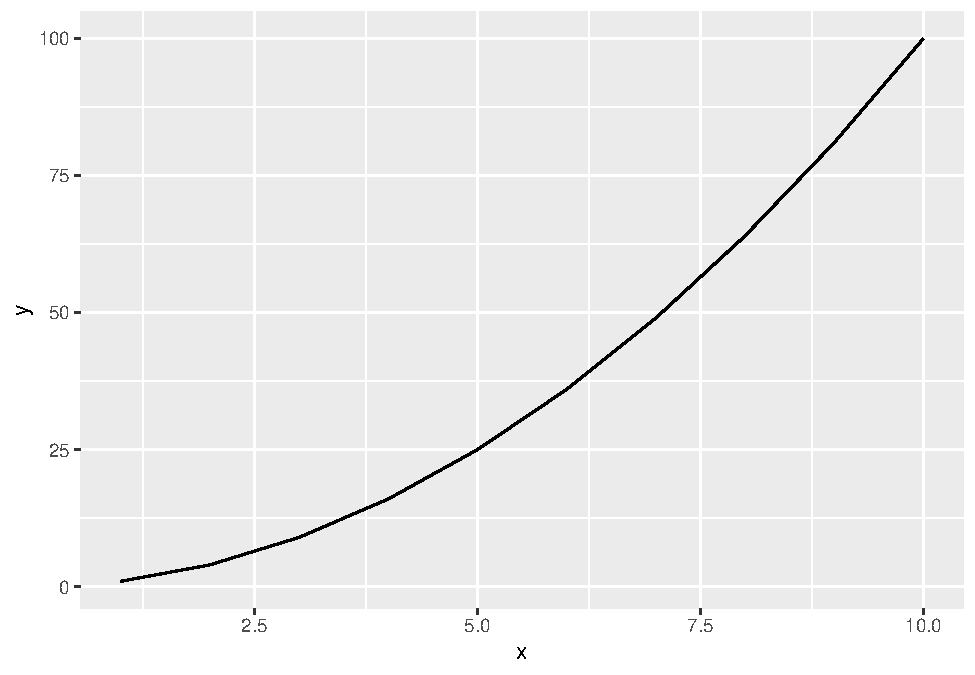
\includegraphics{People_Analytics_Lifecycle_files/figure-latex/unnamed-chunk-53-1.pdf}

The GGally library produces a variety of useful information, including correlation coefficients, bivariate scatterplots, and univariate distributions:

\begin{Shaded}
\begin{Highlighting}[]
\CommentTok{# Load library for correlation visuals}
\KeywordTok{library}\NormalTok{(GGally)}

\CommentTok{# Visualize correlation matrix}
\KeywordTok{ggpairs}\NormalTok{(demographics[, }\KeywordTok{c}\NormalTok{(}\StringTok{"annual_comp"}\NormalTok{, }\StringTok{"age"}\NormalTok{, }\StringTok{"org_tenure"}\NormalTok{, }\StringTok{"job_tenure"}\NormalTok{)])}
\end{Highlighting}
\end{Shaded}

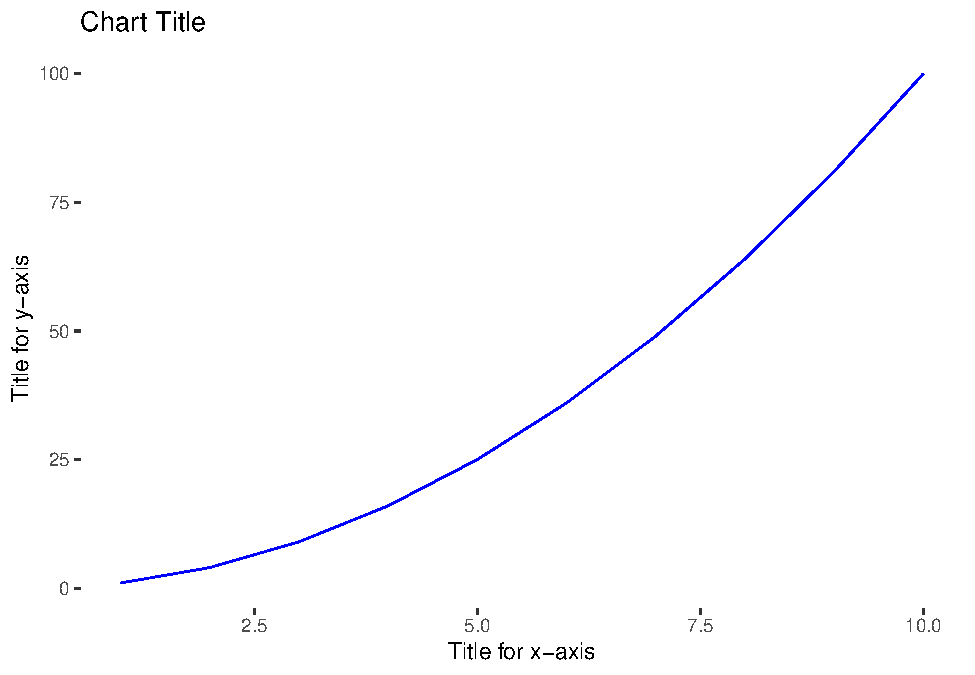
\includegraphics{People_Analytics_Lifecycle_files/figure-latex/unnamed-chunk-54-1.pdf}

As shown in these visuals, there are strong linear associations between variable pairs, such as age and org tenure -- but only for certain values. For example, age is positively correlated with org tenure but beyond about 45 years-old, org tenure varies widely. Understanding the nature of associations will be highly important in the context of linear regression in Chapter \ref{lm}.

It's important to remember that correlation is not causation. Correlations can be spurious (variables related by chance), and drawing conclusions based on bivariate associations alone -- especially in the absence of sound theoretical underpinnings -- can be dangerous.

\begin{figure}

{\centering 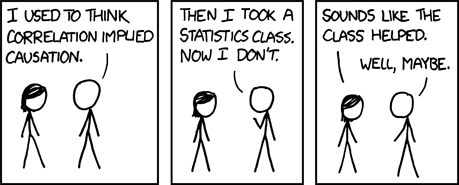
\includegraphics[width=0.75\linewidth]{/Users/craig.starbuck/Library/Mobile Documents/com~apple~CloudDocs/Documents/People Analytics Book/GitHub/peopleanalytics_lifecycle_book/graphics/correlation_comic} 

}

\caption{Correlation comic (Source: www.explainxkcd.com)}\label{fig:corr-comic}
\end{figure}

Here are two examples of nearly perfect correlations between variables for which there is likely no true direct association:

\begin{figure}

{\centering 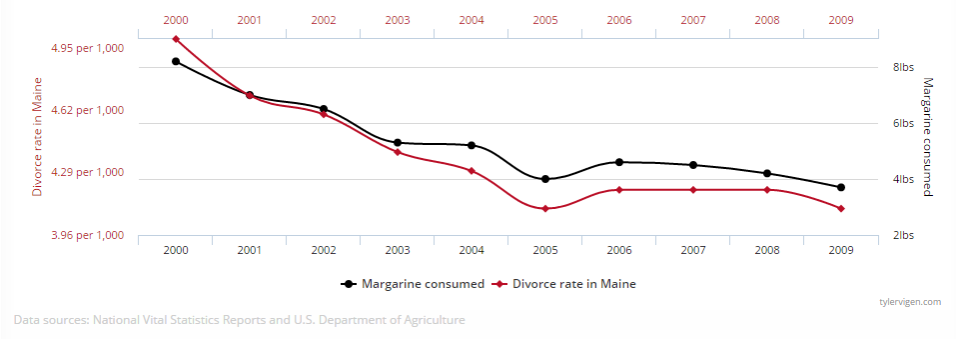
\includegraphics[width=1\linewidth]{/Users/craig.starbuck/Library/Mobile Documents/com~apple~CloudDocs/Documents/People Analytics Book/GitHub/peopleanalytics_lifecycle_book/graphics/spurious_corr_maine_divorce} 

}

\caption{Correlation between Maine Divorce Rate and Margarine Consumption (r = .99)}\label{fig:spur-corr-1}
\end{figure}

\begin{figure}

{\centering 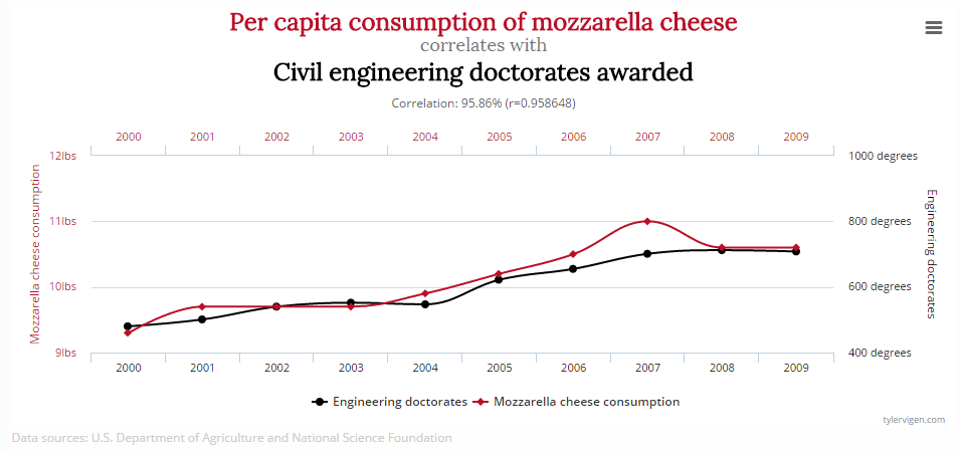
\includegraphics[width=1\linewidth]{/Users/craig.starbuck/Library/Mobile Documents/com~apple~CloudDocs/Documents/People Analytics Book/GitHub/peopleanalytics_lifecycle_book/graphics/spurious_corr_mozzarella_cheese} 

}

\caption{Correlation between Mozzarella Cheese Consumption and Civil Engineering Doctorate Conferrals (r = .96)}\label{fig:spur-corr-2}
\end{figure}

In addition, covariance and correlation alone are not sufficient for determining whether an observed association in sample data is also present in the population. To understand the likelihood that patterns observed in sample data are also present in the larger population of interest, we need to move beyond descriptive measures.

\hypertarget{exercises-2}{%
\section{Exercises}\label{exercises-2}}

\begin{enumerate}
\def\labelenumi{\arabic{enumi}.}
\item
  Which of the following measures of central tendency is least sensitive to extreme values (outliers)?
  A. Median
  B. Mean
  C. Range
\item
  The standard deviation represents the `average' amount by which \(x\) values deviate (or vary) from the mean. A large standard deviation indicates there is considerable spread in the data, whereas a small standard deviation indicates the mean is fairly representative of the data.
  A. True
  B. False
\item
  A positively skewed distribution has its largest allocation to the left and a negative distribution to the right.
  A. True
  B. False
\item
  Large covariance coefficients always indicate strong bivariate associations.
  A. True
  B. False
\item
  Which of the following can be found in boxplots?
  A. Quartiles
  B. Median
  C. Mean
  D. IQR
  E. Outliers
\item
  The 3rd quartile (Q3) is equivalent to the 75th percentile.
  A. True
  B. False
\item
  Which of the following correlation coefficients can be used when evaluating the relationship between a pair of rank-ordered variables?
  A. Pearson's Product Moment
  B. Spearman's Rank
  C. Phi
  D. Point-Biserial
  E. Kendall's Rank
\item
  Which of the following correlation coefficients can be used when evaluating the relationship between a pair of dichotomous variables?
  A. Pearson's Product Moment
  B. Spearman's Rank
  C. Phi
  D. Point-Biserial
  E. Kendall's Rank
\item
  Platykurtic distributions are flat relative to mesokurtic distributions.
  A. True
  B. False
\item
  When using the Pearson method, values down the diagonal of a covariance matrix represent each variable's variance.
  A. True
  B. False
\end{enumerate}

\hypertarget{inf-stats}{%
\chapter{Inferential Statistics}\label{inf-stats}}

The objective of \textbf{inferential statistics} is to make inferences -- with some degree of confidence -- about a population based on available sample data. Several related concepts are fundamental to this goal and will be covered here.

\hypertarget{introduction-to-probability}{%
\section{Introduction to Probability}\label{introduction-to-probability}}

Randomness and uncertainty exist all around us. In \textbf{probability theory}, random phenomena refer to events or experiments whose outcomes cannot be predicted with certainty (Pishro-Nik, 2014). If you've taken a course in probability, there is a good chance you have considered the case of a fair coin flip -- one of the most intuitive applications of probability. In the absence of information on how the coin is flipped, we cannot be certain of the outcome. What we can be certain of is that with a large number of coin flips, the proportion of heads will become increasingly close to 50\%, or \(\frac{1}{2}\).

The \textbf{Law of Large Numbers (LLN)} is an important theorem for building an intuitive understanding of how probability relates to the statistical inference concepts we will cover. In the case of a fair coin flip, it is possible to observe many consecutive heads by chance. This is because small samples can lend to anomalies. However, as the number of flips increases, we will undoubtedly observe an increasing number of tails; we expect a roughly equal number of heads and tails with a large enough number of flips.

\hypertarget{probability-distributions}{%
\subsection{Probability Distributions}\label{probability-distributions}}

\textbf{Probability distributions} are statistical functions that yield the probability of obtaining possible values for a random variable. In other words, the underlying distribution describes how the values of a random variable vary. Probabilities range from 0 to 1, and the sum of all probabilities for all possible values must equal 1.

For example, let's look at how org tenure is distributed across employees. We can understand the general shape of the distribution using descriptive statistics:

\begin{Shaded}
\begin{Highlighting}[]
\CommentTok{# Load library for data wrangling}
\KeywordTok{library}\NormalTok{(dplyr)}

\CommentTok{# Read employee demographics data}
\NormalTok{demographics <-}\StringTok{ }\KeywordTok{read.csv}\NormalTok{(}\StringTok{"https://raw.githubusercontent.com/crstarbuck/peopleanalytics_lifecycle_book/master/data/files/employee_demographics.csv"}\NormalTok{)}

\CommentTok{# Produce descriptive stats for org tenure}
\KeywordTok{summary}\NormalTok{(demographics}\OperatorTok{$}\NormalTok{org_tenure)}
\end{Highlighting}
\end{Shaded}

\begin{verbatim}
##    Min. 1st Qu.  Median    Mean 3rd Qu.    Max. 
##   1.000   5.000   8.000   9.193  13.000  20.000
\end{verbatim}

Comparing the higher mean value of 9.2 to the median value of 8 indicates there are larger values skewing the mean upward which can be seen in the Q3 and max values.

Beyond descriptives, visuals are often helpful in understanding a variable's distribution. As shown in Figure \ref{fig:org-tenure-dist}, it is clear that org tenure is positively skewed, and understanding the shape (or spread) of this distribution enables us to identify which values are most likely in order to estimate the likelihood of different results:

\begin{Shaded}
\begin{Highlighting}[]
\CommentTok{# Load library for data visualization}
\KeywordTok{library}\NormalTok{(ggplot2)}

\CommentTok{# Visualize org tenure distribution}
\KeywordTok{ggplot}\NormalTok{() }\OperatorTok{+}\StringTok{ }
\StringTok{  }\KeywordTok{aes}\NormalTok{(demographics}\OperatorTok{$}\NormalTok{org_tenure) }\OperatorTok{+}\StringTok{ }
\StringTok{  }\KeywordTok{labs}\NormalTok{(}\DataTypeTok{x =} \StringTok{"Org Tenure"}\NormalTok{, }\DataTypeTok{y =} \StringTok{"Density"}\NormalTok{) }\OperatorTok{+}\StringTok{ }
\StringTok{  }\KeywordTok{geom_histogram}\NormalTok{(}\KeywordTok{aes}\NormalTok{(}\DataTypeTok{y =}\NormalTok{ ..density..), }\DataTypeTok{fill =} \StringTok{"#414141"}\NormalTok{) }\OperatorTok{+}
\StringTok{  }\KeywordTok{geom_density}\NormalTok{(}\DataTypeTok{fill =} \StringTok{"#ADD8E6"}\NormalTok{, }\DataTypeTok{alpha =} \FloatTok{0.6}\NormalTok{) }\OperatorTok{+}
\StringTok{  }\KeywordTok{theme_bw}\NormalTok{()}
\end{Highlighting}
\end{Shaded}

\begin{figure}

{\centering 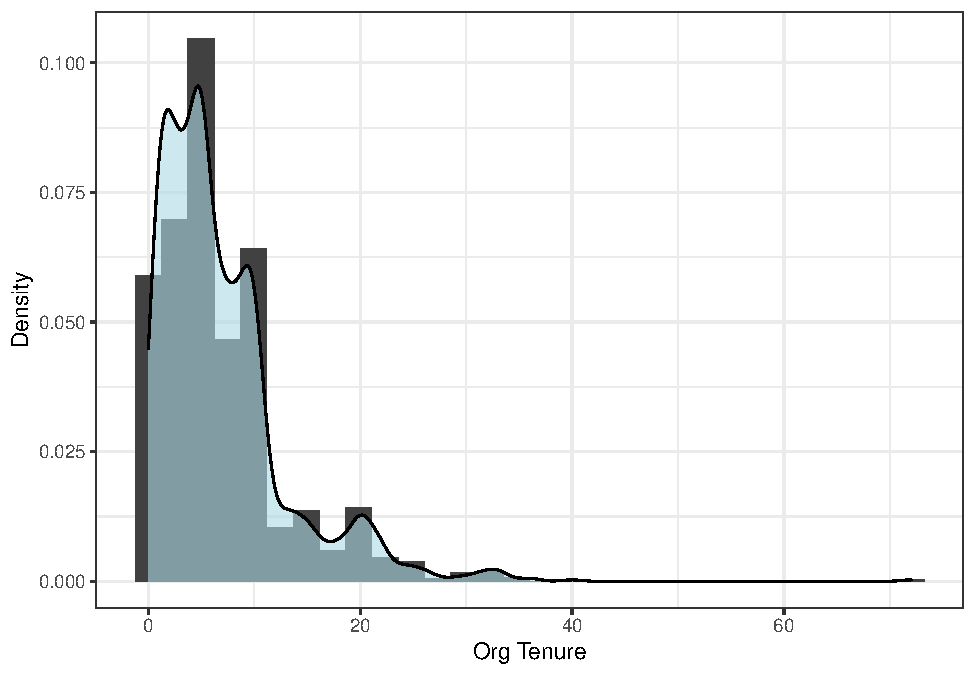
\includegraphics{People_Analytics_Lifecycle_files/figure-latex/org-tenure-dist-1} 

}

\caption{Org Tenure Distribution}\label{fig:org-tenure-dist}
\end{figure}

Just as we grouped variables into disrete and continuous categories in Chapter \ref{measure-sampl}, this is also how probability distributions are categorized. If you read Chapter \ref{measure-sampl}, you likely already have some a priori expectations about the characteristics of discrete and continuous distributions.

The shape of a probability distribution is defined by parameters, which represent its essential properties (e.g., measures of central tendency and spread). These probability distributions underpin the many types of statistical tests covered in this book.

\textbf{Discrete Probability Distributions}

\textbf{Discrete probability distributions}, also known as \textbf{Probability Mass Functions (PMF)}, can be leveraged to model different types of nominal and ordinal variables. Some common discrete distributions include:

\begin{itemize}
\tightlist
\item
  \textbf{Bernoulli}: probability of success or failure for a \emph{single} trial with two outcomes
\item
  \textbf{Binomial}: number of successes and failures in a \emph{sequence} of independent trials with two outcomes (collection of Bernoulli trials)
\item
  \textbf{Multinomial}: generalization of the binomial distribution for experiements with more than two outcomes
\item
  \textbf{Negative Binomial (Pascal)}: a version of the binomial distribution for a \emph{fixed} number of trials (this is positively skewed despite what the name might suggest)
\item
  \textbf{Poisson}: probability of a given number of events occurring over a specified period
\item
  \textbf{Geometric}: special case of the negative binomial distribution that repeats trials until a success is observed (rather than a fixed number of times)
\end{itemize}

A number of functions are available in R to simulate PMFs. The precise shape of a distribution depends on the parameters, but we will simulate and visualize these common PMFs to illustrate differences in the general shape of each. First, let's simulate the distributions by drawing 1,000 random values from each with a specified set of parameters:

\begin{Shaded}
\begin{Highlighting}[]
\CommentTok{# Set seed for reproducible random distribution}
\KeywordTok{set.seed}\NormalTok{(}\DecValTok{1234}\NormalTok{)}

\CommentTok{# Simulate bernoulli distribution}
\NormalTok{bernoulli_dist <-}\StringTok{ }\KeywordTok{rbinom}\NormalTok{(}\DecValTok{1000}\NormalTok{, }\DecValTok{1}\NormalTok{, }\DataTypeTok{prob =} \FloatTok{.5}\NormalTok{)}

\CommentTok{# Simulate binomial distribution}
\CommentTok{# Notice the important difference relative to the Bernoulli simulation (100 trials vs. 1)}
\NormalTok{binomial_dist <-}\StringTok{ }\KeywordTok{rbinom}\NormalTok{(}\DecValTok{1000}\NormalTok{, }\DecValTok{100}\NormalTok{, }\DataTypeTok{prob =} \FloatTok{.5}\NormalTok{) }

\CommentTok{# Simulate negative binomial distribution}
\NormalTok{nbinomial_dist <-}\StringTok{ }\KeywordTok{rnbinom}\NormalTok{(}\DecValTok{1000}\NormalTok{, }\DecValTok{100}\NormalTok{, }\DataTypeTok{prob =} \FloatTok{.5}\NormalTok{) }

\CommentTok{# Simulate multinomial distribution with varying probabilities per level}
\NormalTok{multinomial_dist <-}\StringTok{ }\KeywordTok{rmultinom}\NormalTok{(}\DecValTok{1000}\NormalTok{, }\DecValTok{4}\NormalTok{, }\DataTypeTok{prob =} \KeywordTok{c}\NormalTok{(.}\DecValTok{4}\NormalTok{, }\FloatTok{.3}\NormalTok{, }\FloatTok{.2}\NormalTok{, }\FloatTok{.6}\NormalTok{))}

\CommentTok{# Simulate poisson distribution}
\NormalTok{poisson_dist <-}\StringTok{ }\KeywordTok{rpois}\NormalTok{(}\DecValTok{1000}\NormalTok{, }\DecValTok{10}\NormalTok{) }

\CommentTok{# Simulate geometric distribution}
\NormalTok{geometric_dist <-}\StringTok{ }\KeywordTok{rgeom}\NormalTok{(}\DecValTok{1000}\NormalTok{, }\DataTypeTok{prob =} \FloatTok{.2}\NormalTok{) }
\end{Highlighting}
\end{Shaded}

Next, we will visualize each distribution:

\begin{Shaded}
\begin{Highlighting}[]
\CommentTok{# Load library for arranging visuals}
\KeywordTok{library}\NormalTok{(ggpubr)}

\CommentTok{# Create user-defined function (UDF) to simplify probability distribution visualization}
\CommentTok{# Function arguments: (1) data = object containing random distribution values; (2) type = 'discrete' or 'continuous' probability distribution; and (3) title = name of distribution}
\NormalTok{dist.viz <-}\StringTok{ }\ControlFlowTok{function}\NormalTok{(data, type, title) \{}
  
  \ControlFlowTok{if}\NormalTok{ (type }\OperatorTok{==}\StringTok{ "discrete"}\NormalTok{)\{}
    
    \CommentTok{# Discrete distribution}
\NormalTok{    viz <-}\StringTok{ }\KeywordTok{ggplot}\NormalTok{() }\OperatorTok{+}\StringTok{ }
\StringTok{           }\KeywordTok{aes}\NormalTok{(data) }\OperatorTok{+}\StringTok{ }
\StringTok{           }\KeywordTok{labs}\NormalTok{(}\DataTypeTok{title =} \KeywordTok{paste}\NormalTok{(title), }\DataTypeTok{x =} \StringTok{"x"}\NormalTok{, }\DataTypeTok{y =} \StringTok{"count"}\NormalTok{) }\OperatorTok{+}\StringTok{ }
\StringTok{           }\KeywordTok{geom_histogram}\NormalTok{(}\DataTypeTok{fill =} \StringTok{"#414141"}\NormalTok{) }\OperatorTok{+}
\StringTok{           }\KeywordTok{theme_bw}\NormalTok{() }\OperatorTok{+}
\StringTok{           }\KeywordTok{theme}\NormalTok{(}\DataTypeTok{plot.title =} \KeywordTok{element_text}\NormalTok{(}\DataTypeTok{hjust =} \FloatTok{0.5}\NormalTok{))}
    
\NormalTok{  \} }\ControlFlowTok{else}\NormalTok{ \{}
    
    \CommentTok{# Continuous distribution}
\NormalTok{    viz <-}\StringTok{ }\KeywordTok{ggplot}\NormalTok{() }\OperatorTok{+}\StringTok{ }
\StringTok{           }\KeywordTok{aes}\NormalTok{(data) }\OperatorTok{+}\StringTok{ }
\StringTok{           }\KeywordTok{labs}\NormalTok{(}\DataTypeTok{title =} \KeywordTok{paste}\NormalTok{(title), }\DataTypeTok{x =} \StringTok{"x"}\NormalTok{, }\DataTypeTok{y =} \StringTok{"density"}\NormalTok{) }\OperatorTok{+}\StringTok{ }
\StringTok{           }\KeywordTok{geom_histogram}\NormalTok{(}\KeywordTok{aes}\NormalTok{(}\DataTypeTok{y =}\NormalTok{ ..density..), }\DataTypeTok{fill =} \StringTok{"#414141"}\NormalTok{) }\OperatorTok{+}
\StringTok{           }\KeywordTok{geom_density}\NormalTok{(}\DataTypeTok{fill =} \StringTok{"#ADD8E6"}\NormalTok{, }\DataTypeTok{alpha =} \FloatTok{0.6}\NormalTok{) }\OperatorTok{+}
\StringTok{           }\KeywordTok{theme_bw}\NormalTok{() }\OperatorTok{+}
\StringTok{           }\KeywordTok{theme}\NormalTok{(}\DataTypeTok{plot.title =} \KeywordTok{element_text}\NormalTok{(}\DataTypeTok{hjust =} \FloatTok{0.5}\NormalTok{))}
\NormalTok{  \}}

  \KeywordTok{return}\NormalTok{(viz)}
\NormalTok{\}}

\CommentTok{# Call UDF to build visualizations and store to objects}
\NormalTok{p_bernoulli <-}\StringTok{ }\KeywordTok{dist.viz}\NormalTok{(}\DataTypeTok{data =}\NormalTok{ bernoulli_dist, }\DataTypeTok{type =} \StringTok{"discrete"}\NormalTok{, }\DataTypeTok{title =} \StringTok{"Bernoulli"}\NormalTok{)}
\NormalTok{p_binomial <-}\StringTok{ }\KeywordTok{dist.viz}\NormalTok{(}\DataTypeTok{data =}\NormalTok{ binomial_dist, }\DataTypeTok{type =} \StringTok{"discrete"}\NormalTok{, }\DataTypeTok{title =} \StringTok{"Binomial"}\NormalTok{)}
\NormalTok{p_nbinomial <-}\StringTok{ }\KeywordTok{dist.viz}\NormalTok{(}\DataTypeTok{data =}\NormalTok{ nbinomial_dist, }\DataTypeTok{type =} \StringTok{"discrete"}\NormalTok{, }\DataTypeTok{title =} \StringTok{"Negative Binomial"}\NormalTok{)}
\NormalTok{p_multinomial <-}\StringTok{ }\KeywordTok{dist.viz}\NormalTok{(}\DataTypeTok{data =}\NormalTok{ multinomial_dist, }\DataTypeTok{type =} \StringTok{"discrete"}\NormalTok{, }\DataTypeTok{title =} \StringTok{"Multinomial"}\NormalTok{)}
\NormalTok{p_poisson <-}\StringTok{ }\KeywordTok{dist.viz}\NormalTok{(}\DataTypeTok{data =}\NormalTok{ poisson_dist, }\DataTypeTok{type =} \StringTok{"discrete"}\NormalTok{, }\DataTypeTok{title =} \StringTok{"Poisson"}\NormalTok{)}
\NormalTok{p_geometric <-}\StringTok{ }\KeywordTok{dist.viz}\NormalTok{(}\DataTypeTok{data =}\NormalTok{ geometric_dist, }\DataTypeTok{type =} \StringTok{"discrete"}\NormalTok{, }\DataTypeTok{title =} \StringTok{"Geometric"}\NormalTok{)}
  
\CommentTok{# Display distribution visualizations}
\KeywordTok{ggarrange}\NormalTok{(p_bernoulli, p_binomial, p_nbinomial, p_multinomial, p_poisson, p_geometric,}
          \DataTypeTok{ncol =} \DecValTok{3}\NormalTok{, }\DataTypeTok{nrow =} \DecValTok{2}\NormalTok{)}
\end{Highlighting}
\end{Shaded}

\begin{figure}

{\centering 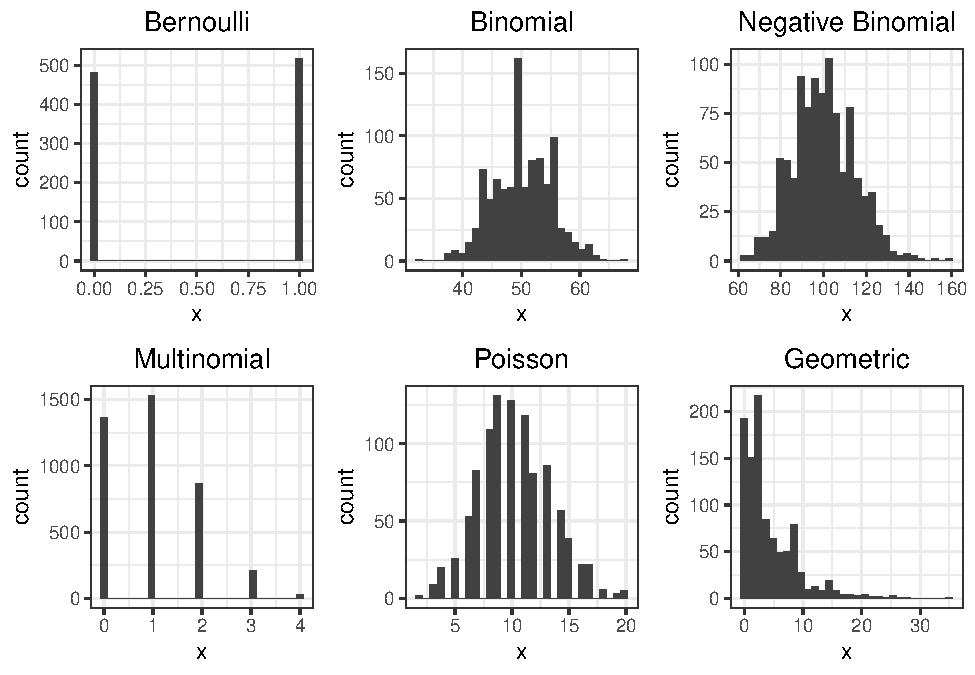
\includegraphics{People_Analytics_Lifecycle_files/figure-latex/discrete-dist-1} 

}

\caption{Discrete Probability Distributions}\label{fig:discrete-dist}
\end{figure}

\textbf{Continuous Probability Distributions}

\textbf{Continuous probability distributions}, also known as \textbf{Probability Density Functions (PDF)}, can be leveraged to model different types of interval and ratio variables. Some common continuous distributions include:

\begin{itemize}
\tightlist
\item
  \textbf{Normal (Gaussian)}: distribution characterized by a mean and standard deviation for which the mean, median, and mode are equal
\item
  \textbf{Uniform}: values of a random variable with equal probabilities of occurring
\item
  \textbf{Log-Normal}: normal distribution of log-transformed values
\item
  \textbf{Student's T}: similar to the normal distribution but with thicker tails (approaches normal as \(n\) increases)
\item
  \textbf{Chi-Square}: similar to the t distribution in that the shape approaches normal as \(n\) increases
\item
  \textbf{F}: developed to examine variances from random samples taken from two independent normal populations
\end{itemize}

A number of functions are available in R to simulate PDFs. While the precise shape of a distribution depends on the parameters, we will simulate and visualize these common PDFs to illustrate differences in the general shape of each. Let's first draw 1,000 random values from each distribution with a specified set of parameters:

\begin{Shaded}
\begin{Highlighting}[]
\CommentTok{# Set seed for reproducible random distribution}
\KeywordTok{set.seed}\NormalTok{(}\DecValTok{1234}\NormalTok{)}

\CommentTok{# Simulate normal distribution}
\NormalTok{normal_dist <-}\StringTok{ }\KeywordTok{rnorm}\NormalTok{(}\DecValTok{1000}\NormalTok{, }\DataTypeTok{mean =} \DecValTok{50}\NormalTok{, }\DataTypeTok{sd =} \DecValTok{5}\NormalTok{)}

\CommentTok{# Simulate log-normal distribution}
\NormalTok{lnormal_dist <-}\StringTok{ }\KeywordTok{rlnorm}\NormalTok{(}\DecValTok{1000}\NormalTok{, }\DataTypeTok{meanlog =} \DecValTok{0}\NormalTok{, }\DataTypeTok{sdlog =} \DecValTok{1}\NormalTok{)}

\CommentTok{# Simulate uniform distribution}
\NormalTok{uniform_dist <-}\StringTok{ }\KeywordTok{runif}\NormalTok{(}\DecValTok{1000}\NormalTok{, }\DataTypeTok{min =} \DecValTok{1}\NormalTok{, }\DataTypeTok{max =} \DecValTok{100}\NormalTok{) }

\CommentTok{# Simulate student's t distribution}
\NormalTok{t_dist <-}\StringTok{ }\KeywordTok{rt}\NormalTok{(}\DecValTok{1000}\NormalTok{, }\DataTypeTok{df =} \DecValTok{5}\NormalTok{)}

\CommentTok{# Simulate chi-square distribution}
\NormalTok{chisq_dist <-}\StringTok{ }\KeywordTok{rchisq}\NormalTok{(}\DecValTok{1000}\NormalTok{, }\DataTypeTok{df =} \DecValTok{5}\NormalTok{)}

\CommentTok{# Simulate F distribution}
\NormalTok{f_dist <-}\StringTok{ }\KeywordTok{rf}\NormalTok{(}\DecValTok{1000}\NormalTok{, }\DataTypeTok{df1 =} \DecValTok{5}\NormalTok{, }\DataTypeTok{df2 =} \DecValTok{200}\NormalTok{)}
\end{Highlighting}
\end{Shaded}

Next, we will visualize each distribution. Since these continuous distributions are probability \emph{density} functions, we will superimpose density plots over each:

\begin{Shaded}
\begin{Highlighting}[]
\CommentTok{# Call UDF to build visualizations and store to objects}
\CommentTok{# Note that as long as the arguments are in the order specified in the function (see our UDF definition above), the argument names do not need to be specified. To illustrate, we will drop the argument names from these function calls:}
\NormalTok{p_normal <-}\StringTok{ }\KeywordTok{dist.viz}\NormalTok{(normal_dist, }\StringTok{"continuous"}\NormalTok{, }\StringTok{"Normal"}\NormalTok{)}
\NormalTok{p_lnormal <-}\StringTok{ }\KeywordTok{dist.viz}\NormalTok{(lnormal_dist, }\StringTok{"continuous"}\NormalTok{, }\StringTok{"Log-Normal"}\NormalTok{)}
\NormalTok{p_uniform <-}\StringTok{ }\KeywordTok{dist.viz}\NormalTok{(uniform_dist, }\StringTok{"continuous"}\NormalTok{, }\StringTok{"Uniform"}\NormalTok{)}
\NormalTok{p_t <-}\StringTok{ }\KeywordTok{dist.viz}\NormalTok{(t_dist, }\StringTok{"continuous"}\NormalTok{, }\StringTok{"Student's T"}\NormalTok{)}
\NormalTok{p_chisq <-}\StringTok{ }\KeywordTok{dist.viz}\NormalTok{(chisq_dist, }\StringTok{"continuous"}\NormalTok{, }\StringTok{"Chi-Square"}\NormalTok{)}
\NormalTok{p_f <-}\StringTok{ }\KeywordTok{dist.viz}\NormalTok{(f_dist, }\StringTok{"continuous"}\NormalTok{, }\StringTok{"F"}\NormalTok{)}

\CommentTok{# Display distribution visualizations}
\KeywordTok{ggarrange}\NormalTok{(p_normal, p_lnormal, p_uniform, p_t, p_chisq, p_f,}
          \DataTypeTok{ncol =} \DecValTok{3}\NormalTok{, }\DataTypeTok{nrow =} \DecValTok{2}\NormalTok{)}
\end{Highlighting}
\end{Shaded}

\begin{figure}

{\centering 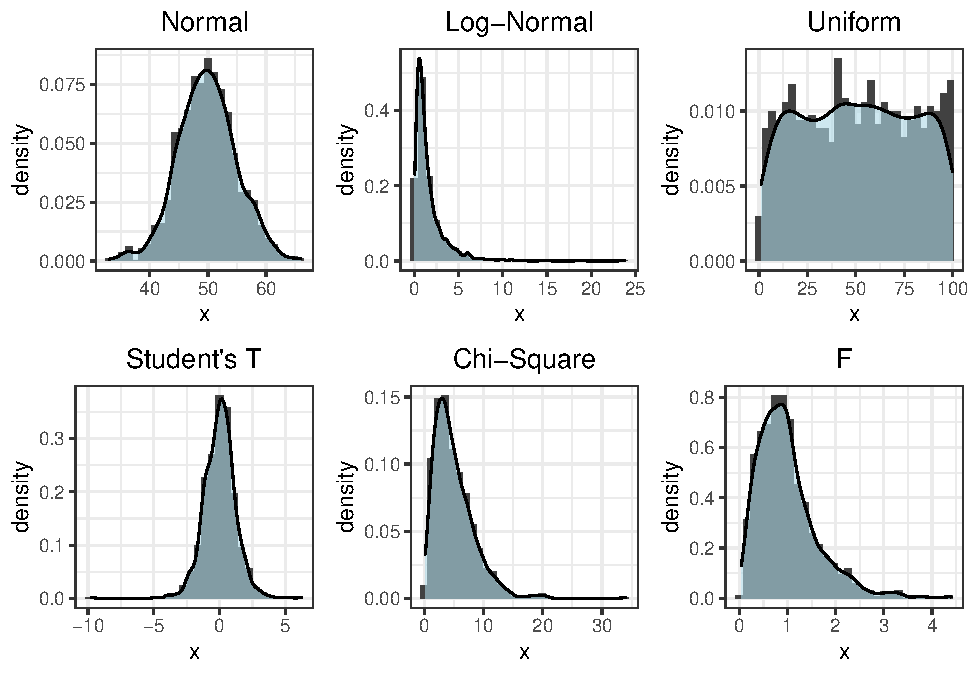
\includegraphics{People_Analytics_Lifecycle_files/figure-latex/continous-dist-1} 

}

\caption{Continuous Probability Distributions}\label{fig:continous-dist}
\end{figure}

The distribution of data is critically important in statistics. The accuracy of many statistical tests is based on assumptions rooted in underlying data distributions, and violating these assumptions can result in serious errors due to misaligned probability distributions. Though there are many more discrete and continuous probability distributions, we will leverage several of these common types to assess the likelihood of differences, effects, and associations in later chapters of this book.

\hypertarget{conditional-probability}{%
\subsection{Conditional Probability}\label{conditional-probability}}

\textbf{Conditional probability} reflects the probability conditioned on the occurrence of a previous event or outcome. For example, we may find that the proportion of heads is greater or less than \(\frac{1}{2}\) with a large number of fair coin flips when the coin is consistently heads up when flipped. The outcome is, therefore, conditioned on the fixed -- rather than random -- positioning of the coin when flipped.

Formally, \textbf{Bayes' Theorem (alternatively, Bayes' Rule)} states that for any two events A and B wherein the probability of A is not 0 (\(P(A) \neq 0\)):

\[ P(A \vert B) = \frac{P(B \vert A) P(A)}{P(B)}, \]

where:

\begin{itemize}
\tightlist
\item
  \(A\) = an event
\item
  \(B\) = another event
\item
  \(P(A|B)\) = conditional probability that event A occurs, given event B occurs (posterior)
\item
  \(P(B|A)\) = conditional probability that event B occurs, given event A occurs (likelihood)
\item
  \(P(B)\) = normalizing constant, constraining the probability distribution to sum to 1 (evidence)
\item
  \(P(A)\) = probability event A occurs before knowing if event B occurs (prior)
\end{itemize}

Bayes' Rule allows us to predict the outcome more accurately by conditioning the probability on known factors rather than assuming all events operate under the same conditions. Bayes' Rule is pervasive in people analytics, as the probability of outcomes can vary widely when conditioned on a person's age, tenure, education, job, perceptions, relationships, and many other factors. For example, if we consider a company with 100 terminations over a 12-month period and average headcount of 1,000, the probability of attrition not conditioned on any other factor is 10\%, or \(\frac{1}{10}\). Aside from trending this probability over time to identify if overall attrition is becoming more or less of a concern, this isn't too helpful at the company level. However, if we condition the probability of attrition on an event -- such as a recent manager exit -- and find that the probability of attrition among those whose manager has left in the last six months is 70\%, or \(\frac{7}{10}\), this is far more actionable (and concerning).

The \textbf{Monty Hall Problem} is an excellent example of how our intuition is often at odds with the laws of conditional probability.

In the classic game show, Let's Make a Deal, Monty Hall asks contestants to choose one of three closed doors. Behind one door is a prize while the other two doors contain nothing. After the contestant selects a door, Monty opens one of the other two doors which does not contain a prize. At this point, there are two closed doors: the door the contestant selected and another for which the content remains unknown. All that is known at this point is that the prize is behind one of the two closed doors.

It is at this juncture that Monty introduces a twist by asking if the contestant would like to switch doors. Most assume that the two closed doors have an equal (50/50) chance of containing the prize, because we generally think of probabilities as independent, random events. However, this is incorrect. Contestants who switch from their original selection have a 66\% chance (rather than 50\%) of winning. This may be counterintuitive, because the brain wants to reduce the problem to a simple coin flip. There is a major difference between the Monty Hall problem and a coin flip; for two outcomes to have the same probability, randomness and independence are required. In the case of the Monty Hall problem, neither assumption is satisfied.

When all three doors are closed, each has the same probability of being selected. The probability of choosing the door with a prize is .33. Monty's knowledge of the door containing the prize does not impact the probability of selecting the winning door. This is because the choice is completely random given we have no information that would increase the probability of a door containing the prize. The process is no longer random when Monty uses his insider knowledge about the prize's location and opens a door he knows does not contain the prize. The probabilities change. Since Monty will never show the door containing the prize, he is careful to always open a door that has nothing behind it. If he was not constrained by the requirement to not reveal the prize's location and instead chose to open one of the remaining doors at random, the probabilities would be equal (and he may end up opening the door that contains the prize).

Seeing is believing, so let's prove this with a simulation in R:

\begin{Shaded}
\begin{Highlighting}[]
\CommentTok{# Set seed for reproducible simulations}
\KeywordTok{set.seed}\NormalTok{(}\DecValTok{12345}\NormalTok{)}

\CommentTok{# Set number of simulations}
\NormalTok{trials =}\StringTok{ }\DecValTok{10000}

\CommentTok{# Store switch/keep decisions}
\NormalTok{decisions =}\StringTok{ }\KeywordTok{c}\NormalTok{(}\StringTok{"switch"}\NormalTok{, }\StringTok{"keep"}\NormalTok{)}

\CommentTok{# Store integer for each door}
\NormalTok{doors =}\StringTok{ }\DecValTok{1}\OperatorTok{:}\DecValTok{3}

\CommentTok{# Initialize empty data frame for results}
\NormalTok{results =}\StringTok{ }\OtherTok{NULL}

\ControlFlowTok{for}\NormalTok{ (n }\ControlFlowTok{in} \DecValTok{1}\OperatorTok{:}\NormalTok{trials)\{}
  
  \ControlFlowTok{for}\NormalTok{ (decision }\ControlFlowTok{in}\NormalTok{ decisions)\{}
    
    \CommentTok{# Select correct door}
\NormalTok{    correct_door <-}\StringTok{ }\KeywordTok{sample}\NormalTok{(doors, }\DecValTok{1}\NormalTok{, }\DataTypeTok{replace =}\NormalTok{ T)}

    \CommentTok{# Contestant chooses a door at random}
\NormalTok{    selected_door <-}\StringTok{ }\KeywordTok{sample}\NormalTok{(doors, }\DecValTok{1}\NormalTok{, }\DataTypeTok{replace =}\NormalTok{ T)}
  
    \CommentTok{# Open door that was neither selected by the contestant nor contains the prize}
    \CommentTok{# Choose one door to open if multiple remain without the prize (i.e., the contestant didn't initially select the door containing the prize)}
\NormalTok{    remaining_doors <-}\StringTok{ }\KeywordTok{which}\NormalTok{(}\OperatorTok{!}\NormalTok{doors }\OperatorTok{==}\StringTok{ }\NormalTok{correct_door }\OperatorTok{&}\StringTok{ }\OperatorTok{!}\NormalTok{doors }\OperatorTok{==}\StringTok{ }\NormalTok{selected_door)}
\NormalTok{    open_door <-}\StringTok{ }\KeywordTok{sample}\NormalTok{(remaining_doors, }\DecValTok{1}\NormalTok{, }\DataTypeTok{replace =}\NormalTok{ T) }
  
    \CommentTok{# Contestant makes decision to switch doors or keep with the originally selected door}
\NormalTok{    selected_door <-}\StringTok{ }\KeywordTok{ifelse}\NormalTok{(decision }\OperatorTok{==}\StringTok{ "switch"}\NormalTok{, }\KeywordTok{which}\NormalTok{(}\OperatorTok{!}\NormalTok{doors }\OperatorTok{==}\StringTok{ }\NormalTok{selected_door }\OperatorTok{&}\StringTok{ }\OperatorTok{!}\NormalTok{doors }\OperatorTok{==}\StringTok{ }\NormalTok{open_door), selected_door)}
    
    \CommentTok{# Store results in data frame}
\NormalTok{    results <-}\StringTok{ }\KeywordTok{rbind}\NormalTok{(results, }\KeywordTok{cbind.data.frame}\NormalTok{(}
                     \DataTypeTok{trial =}\NormalTok{ n,}
                     \DataTypeTok{decision =}\NormalTok{ decision,}
                     \DataTypeTok{result =} \KeywordTok{ifelse}\NormalTok{(correct_door }\OperatorTok{==}\StringTok{ }\NormalTok{selected_door, }\StringTok{"win"}\NormalTok{, }\StringTok{"lose"}\NormalTok{)))}
\NormalTok{  \}}
\NormalTok{\}}

\CommentTok{# Calculate percentage difference in wins for switch vs. keep decisions}
\NormalTok{switch_wins <-}\StringTok{ }\KeywordTok{nrow}\NormalTok{(results[results}\OperatorTok{$}\NormalTok{decision }\OperatorTok{==}\StringTok{ "switch"} \OperatorTok{&}\StringTok{ }\NormalTok{results}\OperatorTok{$}\NormalTok{result }\OperatorTok{==}\StringTok{ "win"}\NormalTok{, ]) }\OperatorTok{/}\StringTok{ }\KeywordTok{nrow}\NormalTok{(results) }\OperatorTok{*}\StringTok{ }\DecValTok{100}
\NormalTok{keep_wins <-}\StringTok{ }\KeywordTok{nrow}\NormalTok{(results[results}\OperatorTok{$}\NormalTok{decision }\OperatorTok{==}\StringTok{ "keep"} \OperatorTok{&}\StringTok{ }\NormalTok{results}\OperatorTok{$}\NormalTok{result }\OperatorTok{==}\StringTok{ "win"}\NormalTok{, ]) }\OperatorTok{/}\StringTok{ }\KeywordTok{nrow}\NormalTok{(results) }\OperatorTok{*}\StringTok{ }\DecValTok{100}
\KeywordTok{round}\NormalTok{((switch_wins }\OperatorTok{-}\StringTok{ }\NormalTok{keep_wins) }\OperatorTok{/}\StringTok{ }\NormalTok{keep_wins }\OperatorTok{*}\StringTok{ }\DecValTok{100}\NormalTok{, }\DecValTok{0}\NormalTok{)}
\end{Highlighting}
\end{Shaded}

\begin{verbatim}
## [1] 45
\end{verbatim}

As we can see, wins occur nearly 50\% more often when contestants switch doors. This exercise hopefully demonstrates the importance of conditional probability and statistical assumptions like randomness. Also, if ever you find yourself playing Let's Make a Deal, switch doors.

\hypertarget{central-limit-theorem}{%
\section{Central Limit Theorem}\label{central-limit-theorem}}

The \textbf{Central Limit Theorem (CLT)} is a mainstay of statistics and probability and fundamental to understanding the mechanics of multivariate inferential analysis techniques we will cover later in this book. The CLT was initially coined by a French-born mathematician named Abraham De Moivre in the 1700s. While initially unpopular, it was later reintroduced and attracted new interest from theorists and academics (Daw \& Pearson, 1972).

The CLT states that the average of independent random variables, when increased in number, tend to follow a normal (or Gaussian) distribution. The distribution of sample means approaches a normal distribution regardless of the shape of the population distribution from which the samples are drawn. This is important because the normal distribution has properties that can be used to test the likelihood that an observed value, difference, or relationship in a sample is also present in the population.

\begin{figure}

{\centering 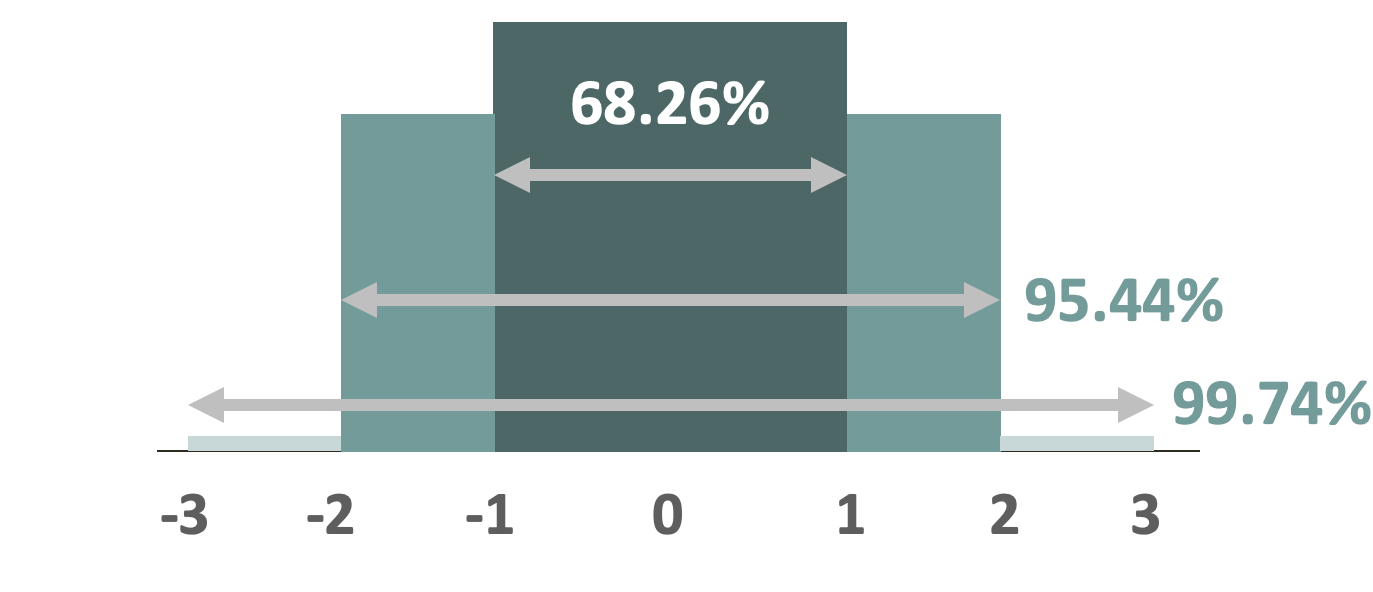
\includegraphics[width=0.75\linewidth]{/Users/craig.starbuck/Library/Mobile Documents/com~apple~CloudDocs/Documents/People Analytics Book/GitHub/peopleanalytics_lifecycle_book/graphics/normal_distribution} 

}

\caption{The Empirical Rule}\label{fig:emp-rule}
\end{figure}

Let's begin with an intuitive example of CLT. Imagine that we have a reliable way to measure how fun a population is on a 100-point scale, where 100 indicates maximum fun (life of the party) and 1 indicates maximum boringness. Consider that a small statistics conference is in progress at a nearby convention center, and there are 40 statisticians in attendance. In a separate room at the same convention center, there is also a group of 40 random people (non-statisticians) who are gathered to discuss some less interesting topic. Our job is to walk into one of the rooms and determine -- based on the ``fun'' factor alone -- whether we have entered the statistics conference or the other, less interesting gathering of non-statisticians.

Instinctively, we already know the statisticians will be more fun than the other group. However, let's assume we need the mean fun score and standard deviation of these two groups for this example. The group of statisticians have, on average, a fun score of 85 with a standard deviation of 2, while the group of non-statisticians are a bit less fun with a mean score of 65 and a standard deviation of 4. With a known population mean and standard deviation, the standard error (the standard deviation of the sample means) provides the ability to calculate the probability that the sample (the room of 40 people) belongs to the population of interest (fellow statisticians).

Herein lies the beauty of the CLT: roughly 68 percent of sample means will lie within one standard error of the population mean, roughly 95 percent within two standard errors of the population mean, and roughly 99 percent within three standard errors of the population mean. Therefore, any room whose members have an average fun score that is not within two standard errors of the population mean (between 81 and 89 for our statisticians) is statistically unlikely to be the group of statisticians for which we are searching. This is because in less than 5 in 100 cases could we randomly draw a `reasonably sized' sample of statisticians with average funness so extremely different from the population average.

Because small samples lend to anomalies, we could -- by chance -- select a single person who happens to fall in the tails (extremely boring or extremely fun); however, as the sample size increases, it becomes more and more likely that the observed average reflects the average of the larger population. It would be virtually impossible (in less than 1 in 100 cases) to draw a random sample of statisticians from the population with average funness that is not within three standard errors of the population mean (between 79 and 91). Therefore, if we find that the room of people have an average fun score of 75, we will likely have far more fun in the other room!

Let's now see the CLT in action by simulating a random uniform population distribution from which we can draw random samples. Remember, the shape of the population distribution does not matter; we could simulate an Exponential, Gamma, Poisson, Binomial, or other distribution and observe the same behavior.

\begin{Shaded}
\begin{Highlighting}[]
\CommentTok{# Set seed for reproducible random distribution}
\KeywordTok{set.seed}\NormalTok{(}\DecValTok{1234}\NormalTok{)}

\CommentTok{# Generate uniform population distribution with 1000 values ranging from 1 to 100}
\NormalTok{rand.unif <-}\StringTok{ }\KeywordTok{runif}\NormalTok{(}\DecValTok{1000}\NormalTok{, }\DataTypeTok{min =} \DecValTok{1}\NormalTok{, }\DataTypeTok{max =} \DecValTok{100}\NormalTok{)}
\end{Highlighting}
\end{Shaded}

\begin{Shaded}
\begin{Highlighting}[]
\CommentTok{# Calculate population mean}
\KeywordTok{mean}\NormalTok{(rand.unif)}
\end{Highlighting}
\end{Shaded}

\begin{verbatim}
## [1] 51.22007
\end{verbatim}

\begin{Shaded}
\begin{Highlighting}[]
\CommentTok{# Calculate population variance}
\NormalTok{N =}\StringTok{ }\KeywordTok{length}\NormalTok{(rand.unif)}
\KeywordTok{var}\NormalTok{(rand.unif) }\OperatorTok{*}\StringTok{ }\NormalTok{(N }\OperatorTok{-}\StringTok{ }\DecValTok{1}\NormalTok{) }\OperatorTok{/}\StringTok{ }\NormalTok{N}
\end{Highlighting}
\end{Shaded}

\begin{verbatim}
## [1] 830.3155
\end{verbatim}

\begin{Shaded}
\begin{Highlighting}[]
\CommentTok{# Produce histogram to visualize population distribution}
\KeywordTok{ggplot}\NormalTok{() }\OperatorTok{+}\StringTok{ }
\StringTok{  }\KeywordTok{aes}\NormalTok{(rand.unif) }\OperatorTok{+}\StringTok{ }
\StringTok{  }\KeywordTok{labs}\NormalTok{(}\DataTypeTok{x =} \StringTok{"x"}\NormalTok{, }\DataTypeTok{y =} \StringTok{"Density"}\NormalTok{) }\OperatorTok{+}\StringTok{ }
\StringTok{  }\KeywordTok{geom_histogram}\NormalTok{(}\KeywordTok{aes}\NormalTok{(}\DataTypeTok{y =}\NormalTok{ ..density..), }\DataTypeTok{fill =} \StringTok{"#414141"}\NormalTok{) }\OperatorTok{+}
\StringTok{  }\KeywordTok{geom_density}\NormalTok{(}\DataTypeTok{fill =} \StringTok{"#ADD8E6"}\NormalTok{, }\DataTypeTok{alpha =} \FloatTok{0.6}\NormalTok{) }\OperatorTok{+}
\StringTok{  }\KeywordTok{theme_bw}\NormalTok{()}
\end{Highlighting}
\end{Shaded}

\begin{figure}

{\centering 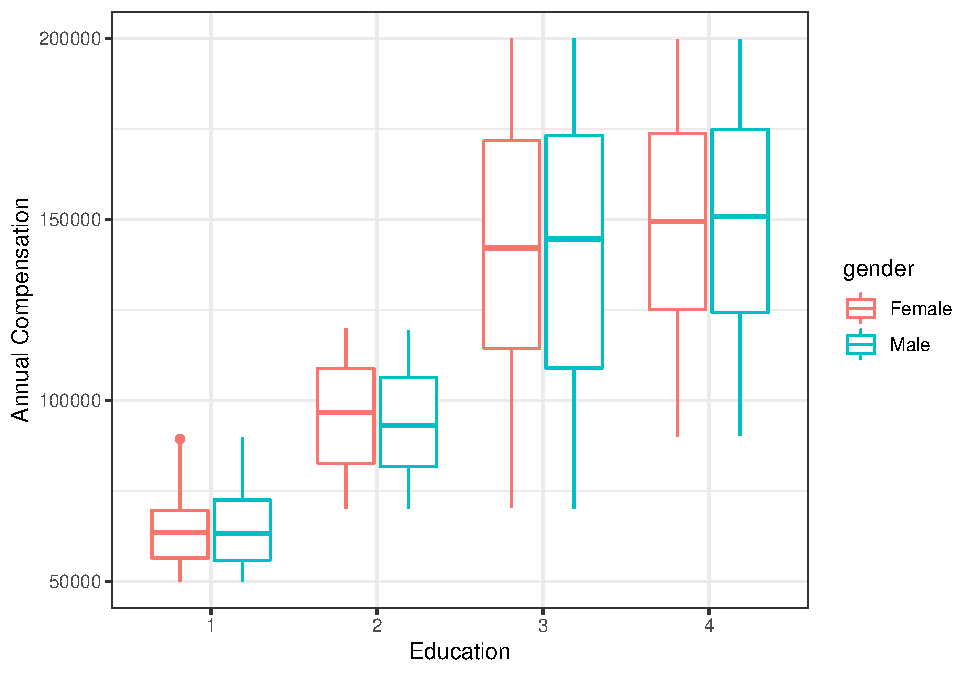
\includegraphics{People_Analytics_Lifecycle_files/figure-latex/unnamed-chunk-62-1} 

}

\caption{Uniform Population Distribution (N = 1000)}\label{fig:unnamed-chunk-62}
\end{figure}

As expected, these randomly generated data are uniformly distributed. Next, we will draw 100 random samples of various sizes and plot the average of each.

\begin{Shaded}
\begin{Highlighting}[]
\CommentTok{# Define number of samples to draw from population distribution}
\NormalTok{samples <-}\StringTok{ }\DecValTok{10000}

\CommentTok{# Populate vector with sample sizes}
\NormalTok{sample_n <-}\StringTok{ }\KeywordTok{c}\NormalTok{(}\DecValTok{1}\OperatorTok{:}\DecValTok{5}\NormalTok{,}\DecValTok{10}\NormalTok{,}\DecValTok{25}\NormalTok{,}\DecValTok{50}\NormalTok{)}

\CommentTok{# Initialize empty data frame to hold sample means}
\NormalTok{sample_means =}\StringTok{ }\OtherTok{NULL}

\CommentTok{# Set seed for reproducible random samples}
\KeywordTok{set.seed}\NormalTok{(}\DecValTok{456}\NormalTok{)}

\CommentTok{# For each n, draw random samples}
\ControlFlowTok{for}\NormalTok{ (n }\ControlFlowTok{in}\NormalTok{ sample_n) \{}
  
  \ControlFlowTok{for}\NormalTok{ (draw }\ControlFlowTok{in} \DecValTok{1}\OperatorTok{:}\NormalTok{samples) \{}
    
      \CommentTok{# Store sample means in data frame}
\NormalTok{      sample_means <-}\StringTok{ }\KeywordTok{rbind}\NormalTok{(sample_means, }\KeywordTok{cbind.data.frame}\NormalTok{(}
                            \DataTypeTok{n =}\NormalTok{ n, }
                            \DataTypeTok{x_bar =} \KeywordTok{mean}\NormalTok{(}\KeywordTok{sample}\NormalTok{(rand.unif, n, }\DataTypeTok{replace =} \OtherTok{TRUE}\NormalTok{, }\DataTypeTok{prob =} \OtherTok{NULL}\NormalTok{))))}
\NormalTok{  \}}
\NormalTok{\}}

\CommentTok{# Produce histograms to visualize distributions of sample means, grouped by n-count}
\NormalTok{sample_means }\OperatorTok\StringTok{ }\KeywordTok{ggplot}\NormalTok{() }\OperatorTok{+}\StringTok{ }
\StringTok{  }\KeywordTok{aes}\NormalTok{(}\DataTypeTok{x =}\NormalTok{ x_bar, }\DataTypeTok{fill =}\NormalTok{ n) }\OperatorTok{+}\StringTok{ }
\StringTok{  }\KeywordTok{labs}\NormalTok{(}\DataTypeTok{x =} \StringTok{"x-bar"}\NormalTok{, }\DataTypeTok{y =} \StringTok{"Density"}\NormalTok{) }\OperatorTok{+}\StringTok{ }
\StringTok{  }\KeywordTok{geom_histogram}\NormalTok{(}\KeywordTok{aes}\NormalTok{(}\DataTypeTok{y =}\NormalTok{ ..density..), }\DataTypeTok{fill =} \StringTok{"#414141"}\NormalTok{) }\OperatorTok{+}
\StringTok{  }\KeywordTok{geom_density}\NormalTok{(}\DataTypeTok{fill =} \StringTok{"#ADD8E6"}\NormalTok{, }\DataTypeTok{alpha =} \FloatTok{0.6}\NormalTok{) }\OperatorTok{+}
\StringTok{  }\KeywordTok{theme_bw}\NormalTok{() }\OperatorTok{+}
\StringTok{  }\KeywordTok{facet_wrap}\NormalTok{(}\OperatorTok{~}\NormalTok{n)}
\end{Highlighting}
\end{Shaded}

\begin{figure}

{\centering 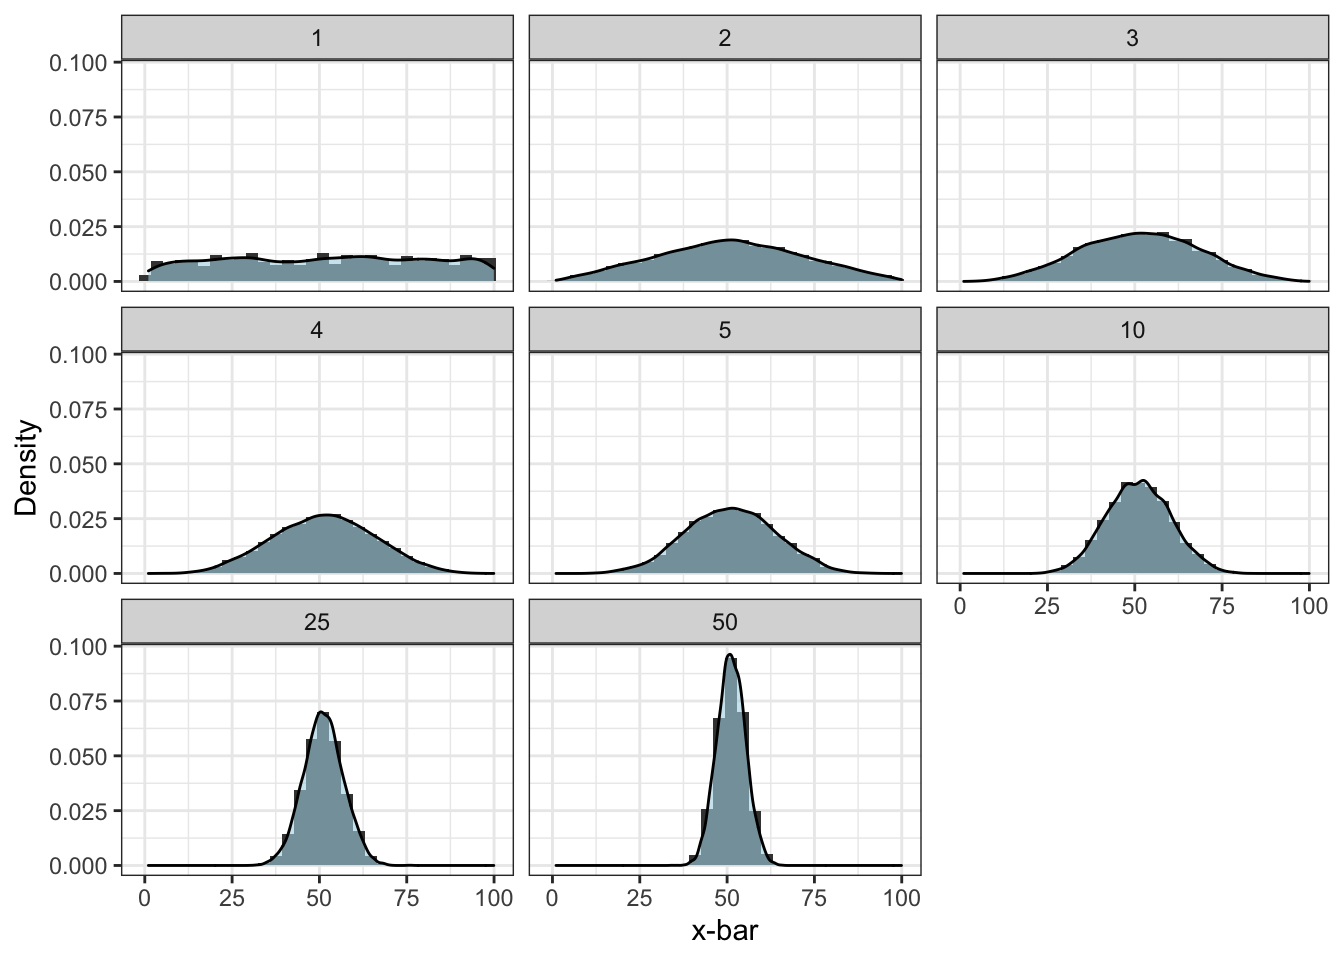
\includegraphics{People_Analytics_Lifecycle_files/figure-latex/unnamed-chunk-63-1} 

}

\caption{Distribution of 10,000 Sample Means of Varied Size}\label{fig:unnamed-chunk-63}
\end{figure}

Per the CLT, we can see that as n increases, the sample means become more normally distributed.

\hypertarget{confidence-intervals}{%
\section{Confidence Intervals}\label{confidence-intervals}}

A \textbf{Confidence Interval (CI)} is a range of values that likely contains the value of an unknown population parameter. These unknown population parameters are often \(\mu\) or \(\sigma\), though we will also leverage CIs in later chapters for regression coefficients, proportions, rates, and differences.

If we draw random samples from a population, we can compute a CI for each sample. Building on the CLT, for a given confidence level (usually 95\%, though 99\% or 90\% are sometimes used), the specified percent of sample intervals is expected to include the estimated population parameter. For example, for a 95\% CI we would expect 19 in every 20 (or 95 in every 100) intervals across the samples to include the true population parameter. This is illustrated in Figure \ref{fig:cis}:

\textbackslash{}begin\{figure\}

\{\centering 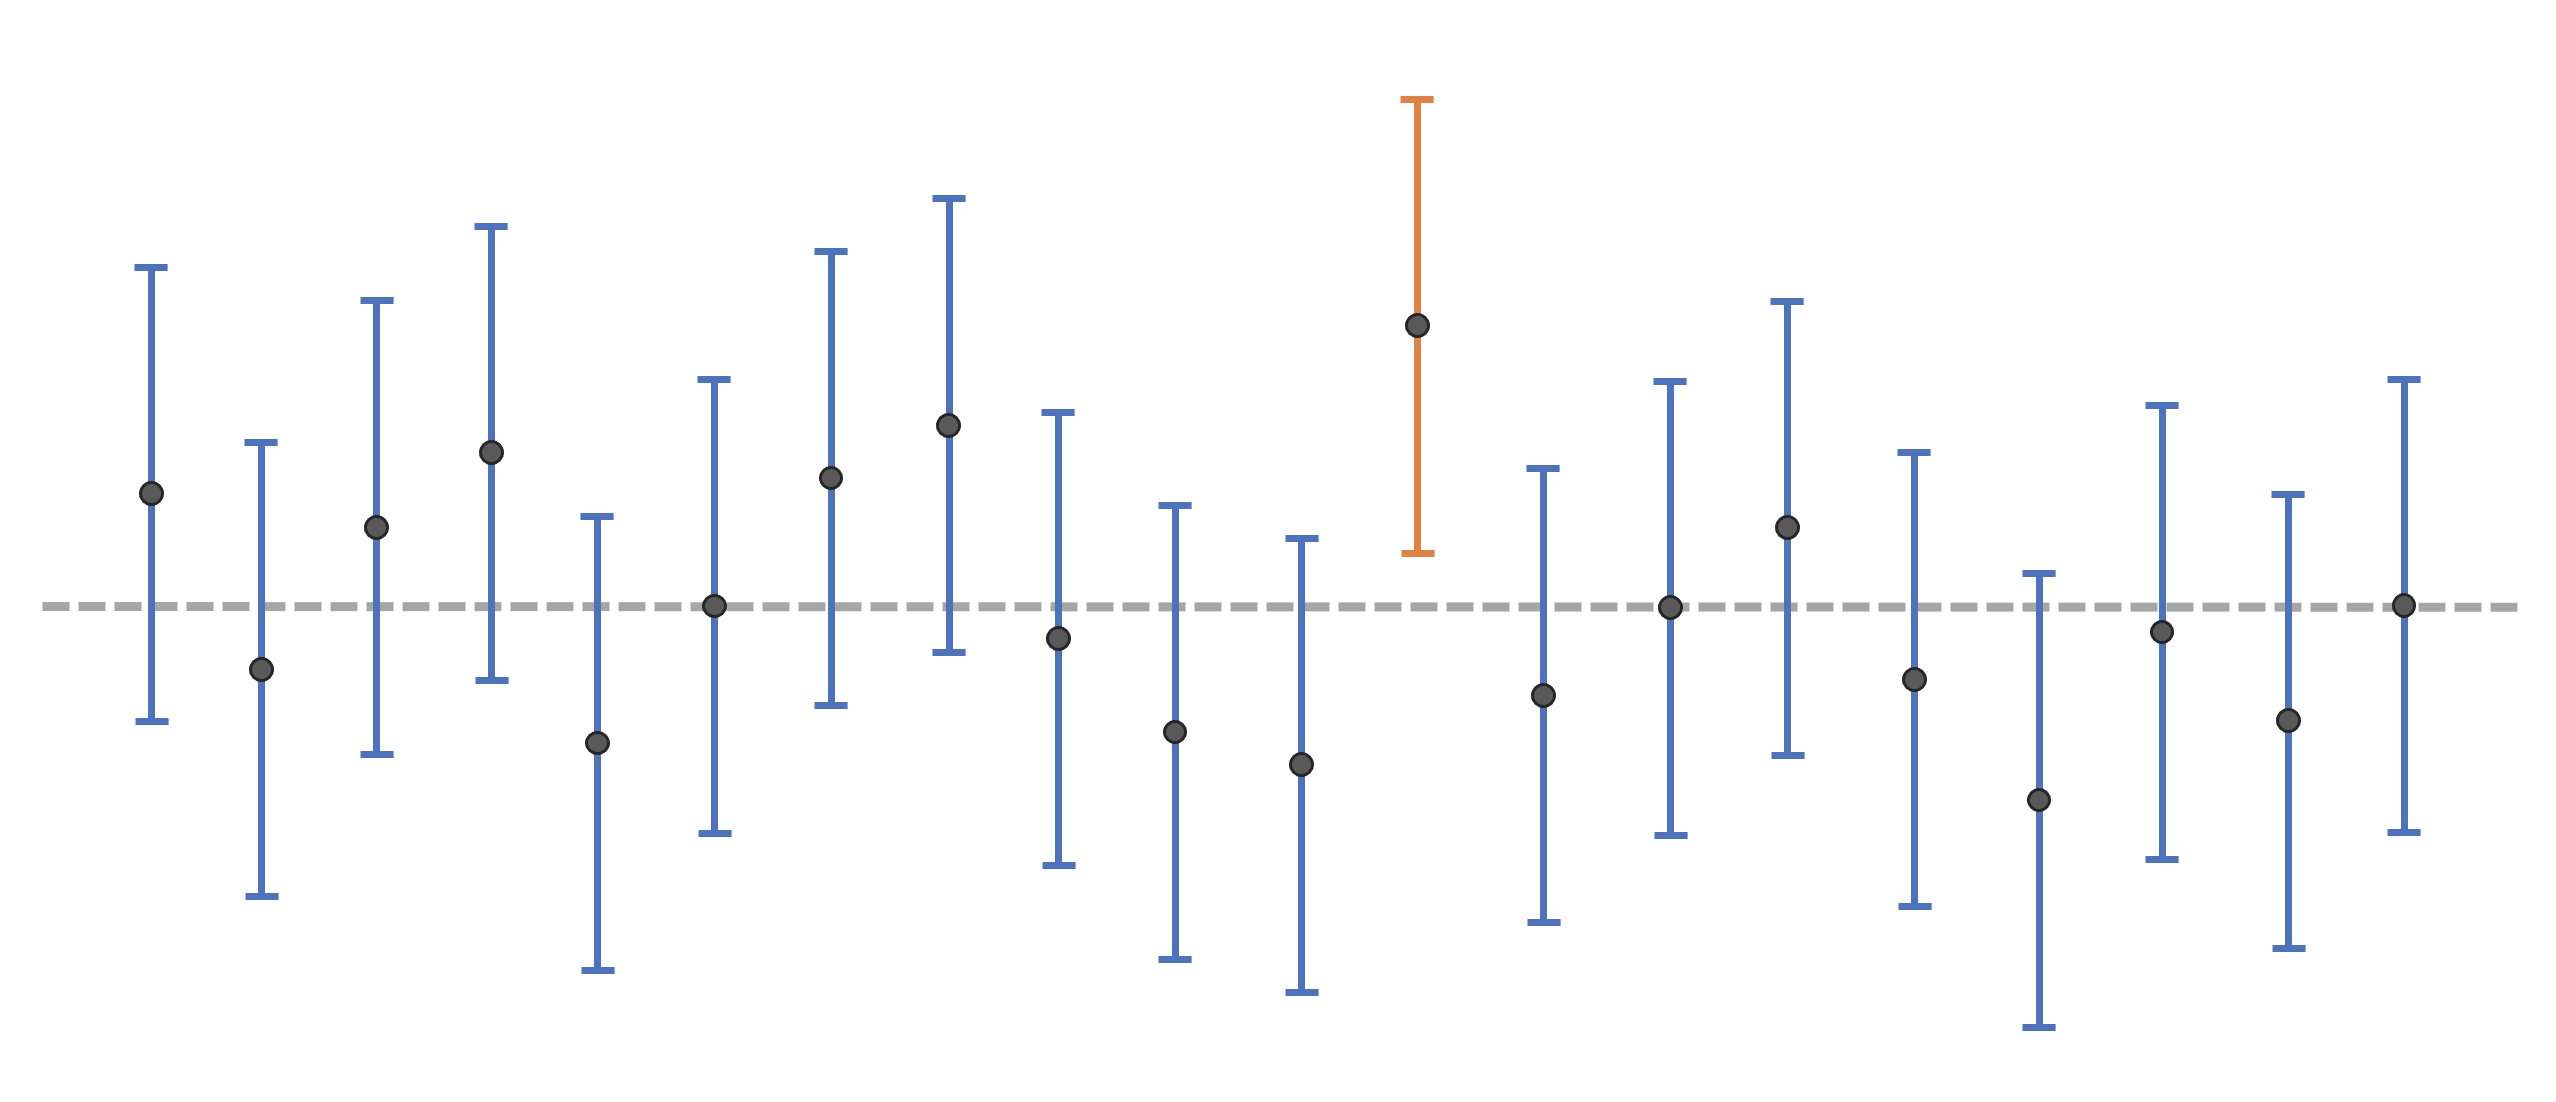
\includegraphics[width=0.75\linewidth]{/Users/craig.starbuck/Library/Mobile Documents/com~apple~CloudDocs/Documents/People Analytics Book/GitHub/peopleanalytics_lifecycle_book/graphics/confidence_intervals}

\}

\textbackslash{}caption\{Intervals for 95\% Confidence Level\}\label{fig:cis}
\textbackslash{}end\{figure\}

It is important to note that CIs should not be applied to the distribution of sample values; CIs relate to \emph{population parameters}. A common misinterpretation of a CI is that it represents an interval within which a certain percent of sample values exist, and this is inaccurate. Because this misinterpretation is so prevalent, there is a good chance you will be tested on your understanding of CIs when applying to positions involving statistical analyses!

A related concept that is fundamental to estimating CIs is the \textbf{standard error (SE)}, which is the standard deviation of sample means. While the standard deviation is a measure of variability for a random variable, the variability captured by the SE reflects how well a sample represents the population. Since sample statistics will approach the actual population parameters as the size of the sample increases, the SE and sample size are inversely related; that is, the SE decreases as the sample size increases. The SE is defined by:

\[ SE = \frac{\sigma}{\sqrt{n}} \]

Since the CLT is fundamental to inferential statistics, let's validate that our simulated distribution of sample means adheres to the properties of normally distributed data per the Empirical Rule:

\begin{Shaded}
\begin{Highlighting}[]
\CommentTok{# Store sample means with n = 50}
\NormalTok{x_bars <-}\StringTok{ }\NormalTok{sample_means[sample_means}\OperatorTok{$}\NormalTok{n }\OperatorTok{==}\StringTok{ }\DecValTok{50}\NormalTok{, }\StringTok{"x_bar"}\NormalTok{]}

\CommentTok{# Store sample size}
\NormalTok{n <-}\StringTok{ }\KeywordTok{length}\NormalTok{(x_bars)}

\CommentTok{# Calculate percent of sample means within +/- 2 SEs}
\KeywordTok{length}\NormalTok{(x_bars[x_bars }\OperatorTok{<}\StringTok{ }\KeywordTok{mean}\NormalTok{(x_bars) }\OperatorTok{+}\StringTok{ }\DecValTok{2} \OperatorTok{*}\StringTok{ }\KeywordTok{sd}\NormalTok{(x_bars) }\OperatorTok{&}\StringTok{ }\NormalTok{x_bars }\OperatorTok{>}\StringTok{ }\KeywordTok{mean}\NormalTok{(x_bars) }\OperatorTok{-}\StringTok{ }\DecValTok{2} \OperatorTok{*}\StringTok{ }\KeywordTok{sd}\NormalTok{(x_bars)]) }\OperatorTok{/}\StringTok{ }\NormalTok{n }\OperatorTok{*}\StringTok{ }\DecValTok{100}
\end{Highlighting}
\end{Shaded}

\begin{verbatim}
## [1] 95.35
\end{verbatim}

95\% of sample means are within 2 SEs, which is what we expect per the characteristics of the normal distribution.

\begin{Shaded}
\begin{Highlighting}[]
\CommentTok{# Calculate percent of sample means within +/- 3 SEs}
\KeywordTok{length}\NormalTok{(x_bars[x_bars }\OperatorTok{<}\StringTok{ }\KeywordTok{mean}\NormalTok{(x_bars) }\OperatorTok{+}\StringTok{ }\DecValTok{3} \OperatorTok{*}\StringTok{ }\KeywordTok{sd}\NormalTok{(x_bars) }\OperatorTok{&}\StringTok{ }\NormalTok{x_bars }\OperatorTok{>}\StringTok{ }\KeywordTok{mean}\NormalTok{(x_bars) }\OperatorTok{-}\StringTok{ }\DecValTok{3} \OperatorTok{*}\StringTok{ }\KeywordTok{sd}\NormalTok{(x_bars)]) }\OperatorTok{/}\StringTok{ }\NormalTok{n }\OperatorTok{*}\StringTok{ }\DecValTok{100}
\end{Highlighting}
\end{Shaded}

\begin{verbatim}
## [1] 99.79
\end{verbatim}

Nearly all of the sample means are within 3 SEs, indicating that it would be highly unlikely -- nearly impossible even -- to observe a sample mean `from the same population' that falls outside this interval.

Now, let's illustrate the relationship between CIs and standard errors using sample data from our uniform population distribution. In our example, both \(\mu\) and \(\sigma\) are known and our sample size \(n\) is at least 30; therefore, we can use a \textbf{Z-Test} to calculate the 95\% CI. A \(z\) score of 1.96 corresponds to the 95\% CI for a two-tailed distribution; that is, we are looking for significantly different values in either the larger or smaller direction. The 95\% CI represents the range of values we would expect to include \(\mu\) in at least 95 of 100 random samples taken from the population.

The CI in this case is defined by:

\[ CI = \bar{x} \pm z_{\alpha/_2} \frac{\sigma}{\sqrt{n}} \]

Let's randomly take \(n\) = 100 from the population, and compute sample statistics to estimate the 95\% CI:

\begin{Shaded}
\begin{Highlighting}[]
\CommentTok{# Set seed for reproducible random samples}
\KeywordTok{set.seed}\NormalTok{(}\DecValTok{456}\NormalTok{)}

\CommentTok{# Sample 100 values from uniform population distribution}
\NormalTok{x <-}\StringTok{ }\KeywordTok{sample}\NormalTok{(rand.unif, }\DecValTok{100}\NormalTok{, }\DataTypeTok{replace =} \OtherTok{TRUE}\NormalTok{, }\DataTypeTok{prob =} \OtherTok{NULL}\NormalTok{)}

\CommentTok{# Calculate 95% CI}
\NormalTok{ci95_lower_bound <-}\StringTok{ }\KeywordTok{mean}\NormalTok{(x) }\OperatorTok{-}\StringTok{ }\FloatTok{1.96} \OperatorTok{*}\StringTok{ }\NormalTok{(}\KeywordTok{sd}\NormalTok{(x) }\OperatorTok{/}\StringTok{ }\KeywordTok{sqrt}\NormalTok{(}\DecValTok{100}\NormalTok{))}
\NormalTok{ci95_upper_bound <-}\StringTok{ }\KeywordTok{mean}\NormalTok{(x) }\OperatorTok{+}\StringTok{ }\FloatTok{1.96} \OperatorTok{*}\StringTok{ }\NormalTok{(}\KeywordTok{sd}\NormalTok{(x) }\OperatorTok{/}\StringTok{ }\KeywordTok{sqrt}\NormalTok{(}\DecValTok{100}\NormalTok{))}
\end{Highlighting}
\end{Shaded}

\begin{Shaded}
\begin{Highlighting}[]
\CommentTok{# Print lower bound for 95% CI}
\NormalTok{ci95_lower_bound}
\end{Highlighting}
\end{Shaded}

\begin{verbatim}
## [1] 47.90733
\end{verbatim}

\begin{Shaded}
\begin{Highlighting}[]
\CommentTok{# Print upper bound for 95% CI}
\NormalTok{ci95_upper_bound}
\end{Highlighting}
\end{Shaded}

\begin{verbatim}
## [1] 58.98773
\end{verbatim}

Our known \(\mu\) is 51.2, which is covered by our 95\% CI (47.9 - 59.0). Per the CLT, in less than 5\% of cases would we expect to draw a random sample from the population that results in a 95\% CI which does not include \(\mu\). Note that our CI narrows with larger samples since our confidence that the range includes \(\mu\) increases with more data.

Next, let's look at a 99\% CI. We will enter 2.576 for \(z\):

\begin{Shaded}
\begin{Highlighting}[]
\CommentTok{# Calculate 99% CI}
\NormalTok{ci99_lower_bound <-}\StringTok{ }\KeywordTok{mean}\NormalTok{(x) }\OperatorTok{-}\StringTok{ }\FloatTok{2.576} \OperatorTok{*}\StringTok{ }\NormalTok{(}\KeywordTok{sd}\NormalTok{(x) }\OperatorTok{/}\StringTok{ }\KeywordTok{sqrt}\NormalTok{(}\DecValTok{100}\NormalTok{))}
\NormalTok{ci99_upper_bound <-}\StringTok{ }\KeywordTok{mean}\NormalTok{(x) }\OperatorTok{+}\StringTok{ }\FloatTok{2.576} \OperatorTok{*}\StringTok{ }\NormalTok{(}\KeywordTok{sd}\NormalTok{(x) }\OperatorTok{/}\StringTok{ }\KeywordTok{sqrt}\NormalTok{(}\DecValTok{100}\NormalTok{))}
\end{Highlighting}
\end{Shaded}

\begin{Shaded}
\begin{Highlighting}[]
\CommentTok{# Print lower bound for 99% CI}
\NormalTok{ci99_lower_bound}
\end{Highlighting}
\end{Shaded}

\begin{verbatim}
## [1] 46.16612
\end{verbatim}

\begin{Shaded}
\begin{Highlighting}[]
\CommentTok{# Print upper bound for 99% CI}
\NormalTok{ci99_upper_bound}
\end{Highlighting}
\end{Shaded}

\begin{verbatim}
## [1] 60.72893
\end{verbatim}

Like the 95\% CI, this slightly wider 99\% CI (46.2 - 60.7) also includes our \(\mu\) of 51.2.

If \(\sigma\) is not known, and/or we have a small sample (\(n\) \textless{} 30), we need to use a \textbf{T-Test} to calculate the CIs. In a people analytics setting, the reality is that population parameters are often unknown. For example, if we knew how engagement scores vary in the employee population, there would be no need to survey a sample of employees and make inferences about said population.

As we will see, the T-Test underpins many statistical tests and models germane to the people analytics discipline since we are often working with small datasets, so it is important to understand the mechanics. As shown in Figure \ref{fig:t-distribution}, the \(t\) distribution is increasingly wider and shorter relative to the normal distribution as the sample size decreases; this is also characteristic of the sampling distribution of means for smaller samples we observed in our CLT example. Specifically, \textbf{degrees of freedom (df)} is used to determine the shape of the probability distribution. Degrees of freedom represents the number of observations in the data that are free to vary when estimating statistical parameters, which is a function of the sample size (\(n - 1\)). For example, if we could choose 1 of 5 projects to work on each day between Monday and Friday, we would only be able to \emph{choose} 4 out of the 5 days; on Friday, only 1 project would remain to be selected, so our degrees of freedom (the number of days in which we have a choice between projects) would be 4.

\begin{figure}

{\centering 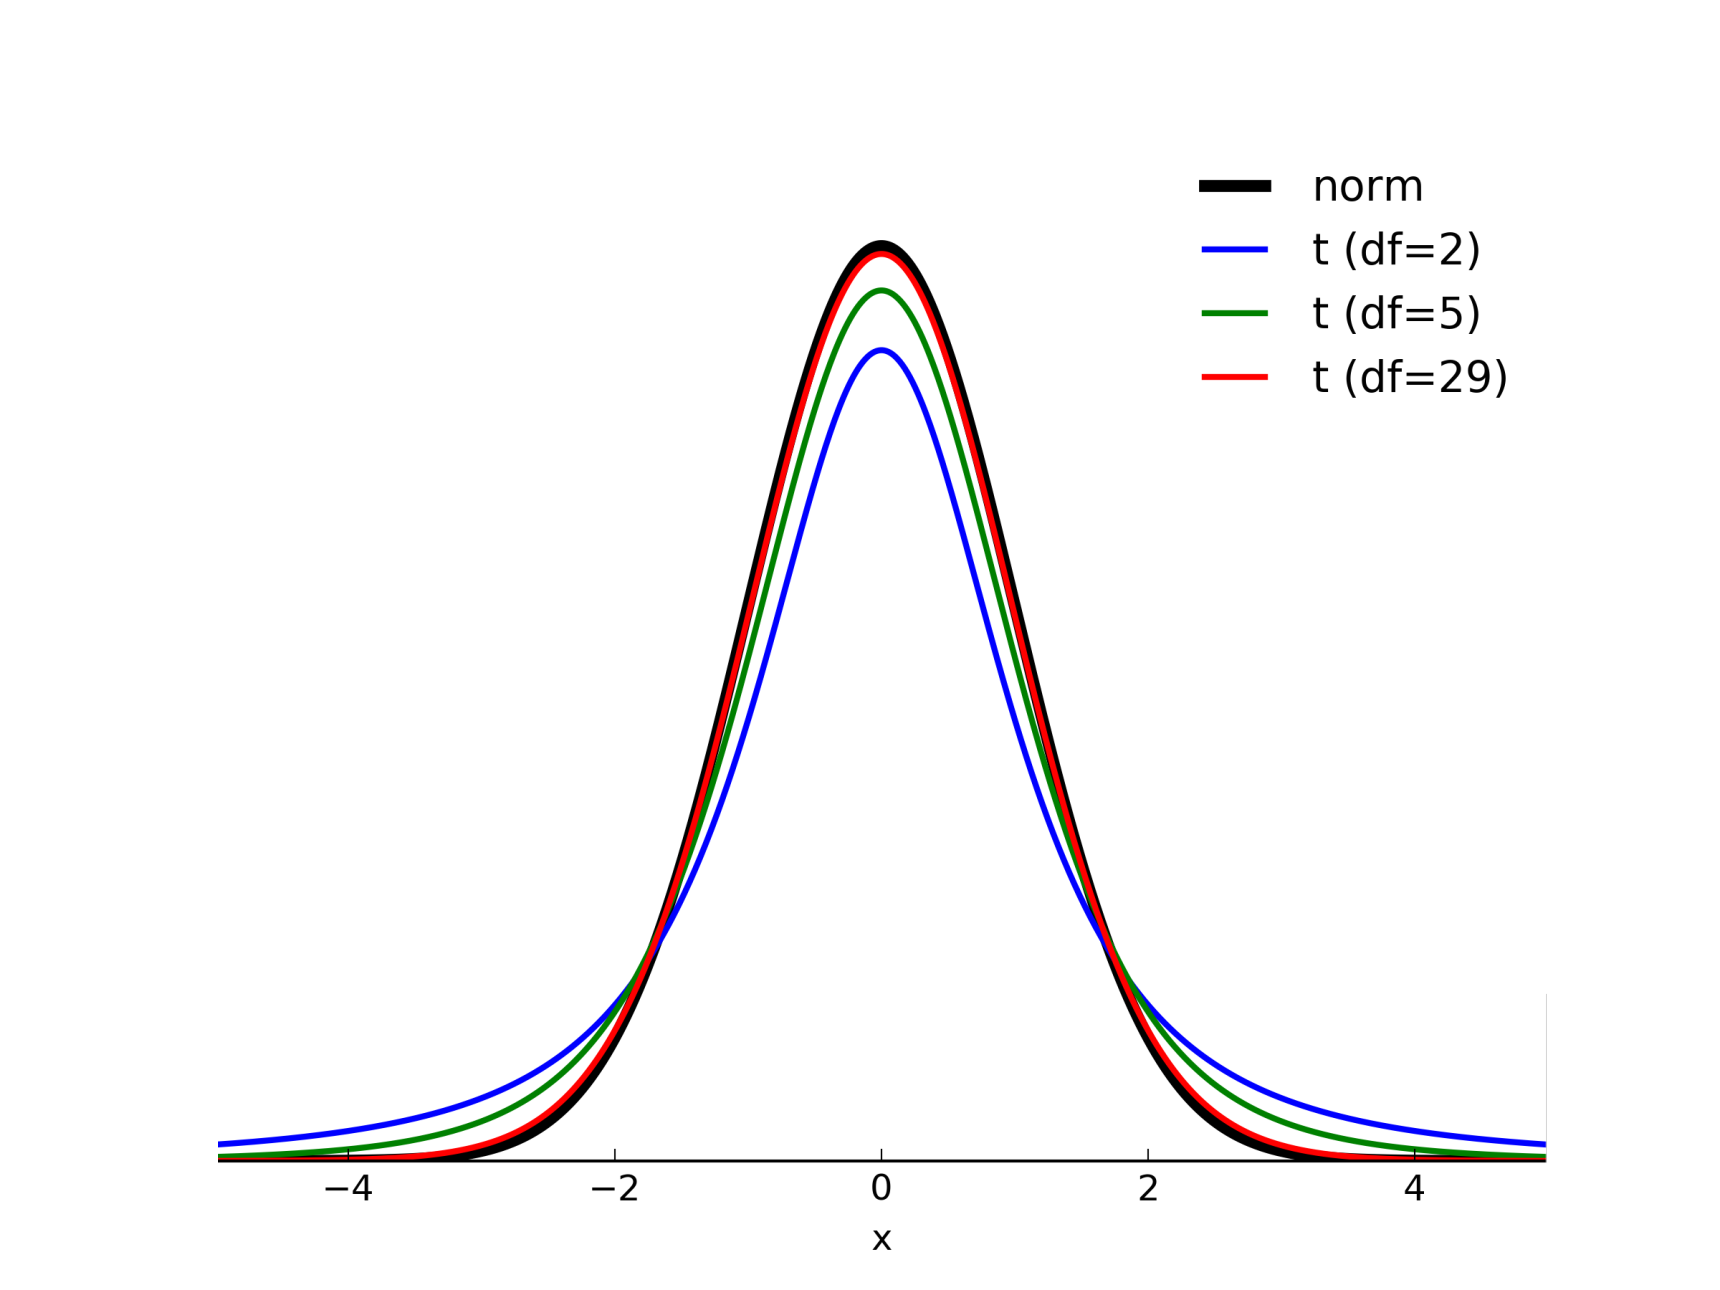
\includegraphics[width=0.5\linewidth]{/Users/craig.starbuck/Library/Mobile Documents/com~apple~CloudDocs/Documents/People Analytics Book/GitHub/peopleanalytics_lifecycle_book/graphics/t_distribution} 

}

\caption{t Distribution Shape by Degrees of Freedom}\label{fig:t-distribution}
\end{figure}

When estimating the CI for smaller samples, we need to leverage the wider, more platykurtic \(t\) distribution to achieve greater accuracy. Therefore, the CI for a two-tailed test in this case is defined by:

\[ CI = \bar{x} \pm t_{\alpha/_2} \frac{\sigma}{\sqrt{n}} \]

Let's compare CIs calculated using a T-Test to those calculated using the Z-Test. While a fixed \(z\) score can be used for each CI level when \(n\) \textgreater{} 30, the \(t\) statistic varies based on both the CI level and \(df\). Though R will determine the correct \(t\) statistic for us, let's reference the table shown in Figure \ref{fig:t-crit} to manually lookup the \(t\) statistic:

\begin{figure}

{\centering 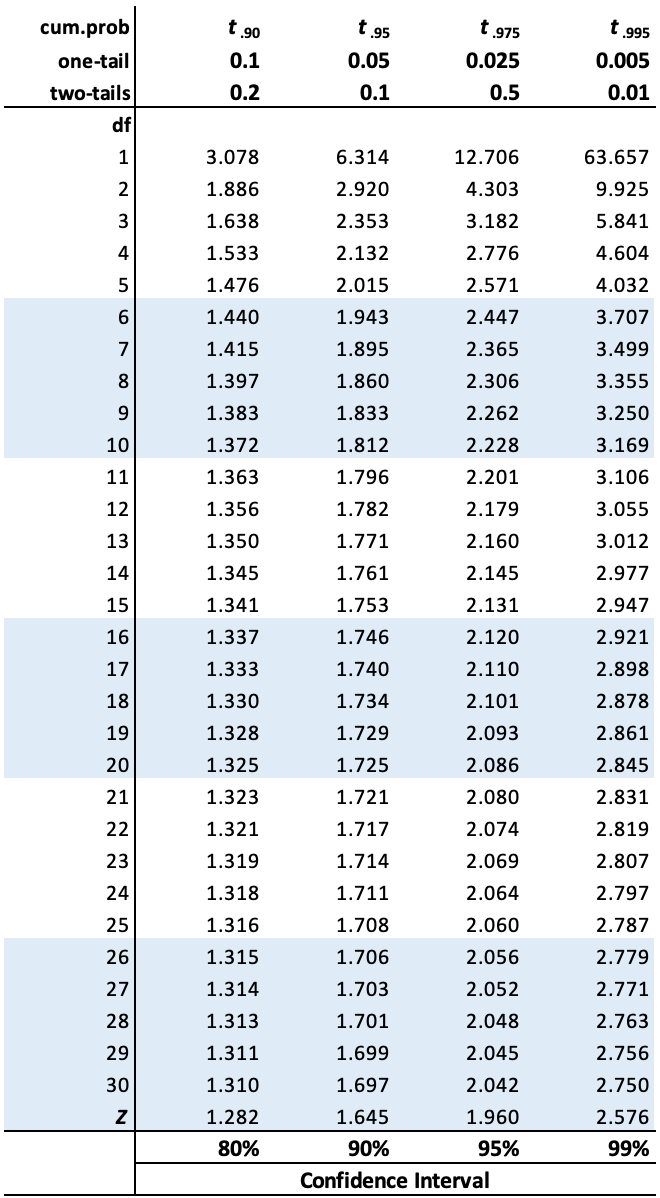
\includegraphics[width=0.5\linewidth]{/Users/craig.starbuck/Library/Mobile Documents/com~apple~CloudDocs/Documents/People Analytics Book/GitHub/peopleanalytics_lifecycle_book/graphics/t-table} 

}

\caption{Critical Values of Student's t Distribution}\label{fig:t-crit}
\end{figure}

For illustrative purposes, let's draw a smaller sample of \(n\) = 25 from our uniform population distribution and calculate the 95\% CI using the \(t\) statistic from the table (\(df\) = 24). The \(t\) statistic for this CI and \(df\) is 2.064:

\begin{Shaded}
\begin{Highlighting}[]
\CommentTok{# Set seed for reproducible random samples}
\KeywordTok{set.seed}\NormalTok{(}\DecValTok{456}\NormalTok{)}

\CommentTok{# Sample 25 values from uniform population distribution}
\NormalTok{x <-}\StringTok{ }\KeywordTok{sample}\NormalTok{(rand.unif, }\DecValTok{25}\NormalTok{, }\DataTypeTok{replace =} \OtherTok{TRUE}\NormalTok{, }\DataTypeTok{prob =} \OtherTok{NULL}\NormalTok{)}

\CommentTok{# Calculate 95% CI}
\NormalTok{ci95_lower_bound <-}\StringTok{ }\KeywordTok{mean}\NormalTok{(x) }\OperatorTok{-}\StringTok{ }\FloatTok{2.064} \OperatorTok{*}\StringTok{ }\NormalTok{(}\KeywordTok{sd}\NormalTok{(x) }\OperatorTok{/}\StringTok{ }\KeywordTok{sqrt}\NormalTok{(}\DecValTok{25}\NormalTok{))}
\NormalTok{ci95_upper_bound <-}\StringTok{ }\KeywordTok{mean}\NormalTok{(x) }\OperatorTok{+}\StringTok{ }\FloatTok{2.064} \OperatorTok{*}\StringTok{ }\NormalTok{(}\KeywordTok{sd}\NormalTok{(x) }\OperatorTok{/}\StringTok{ }\KeywordTok{sqrt}\NormalTok{(}\DecValTok{25}\NormalTok{))}
\end{Highlighting}
\end{Shaded}

\begin{Shaded}
\begin{Highlighting}[]
\CommentTok{# Print lower bound for 95% CI}
\NormalTok{ci95_lower_bound}
\end{Highlighting}
\end{Shaded}

\begin{verbatim}
## [1] 35.24305
\end{verbatim}

\begin{Shaded}
\begin{Highlighting}[]
\CommentTok{# Print upper bound for 95% CI}
\NormalTok{ci95_upper_bound}
\end{Highlighting}
\end{Shaded}

\begin{verbatim}
## [1] 59.60959
\end{verbatim}

As expected, the 95\% CI using the \(t\) statistic is much wider (35.2 - 59.6), acknowledging the increased uncertainty in estimating population parameters given the limited information in this smaller sample. To increase our confidence to the 99\% level, the interval widens even further (30.9 - 63.9):

\begin{Shaded}
\begin{Highlighting}[]
\CommentTok{# Calculate 99% CI}
\NormalTok{ci99_lower_bound <-}\StringTok{ }\KeywordTok{mean}\NormalTok{(x) }\OperatorTok{-}\StringTok{ }\FloatTok{2.797} \OperatorTok{*}\StringTok{ }\NormalTok{(}\KeywordTok{sd}\NormalTok{(x) }\OperatorTok{/}\StringTok{ }\KeywordTok{sqrt}\NormalTok{(}\DecValTok{25}\NormalTok{))}
\NormalTok{ci99_upper_bound <-}\StringTok{ }\KeywordTok{mean}\NormalTok{(x) }\OperatorTok{+}\StringTok{ }\FloatTok{2.797} \OperatorTok{*}\StringTok{ }\NormalTok{(}\KeywordTok{sd}\NormalTok{(x) }\OperatorTok{/}\StringTok{ }\KeywordTok{sqrt}\NormalTok{(}\DecValTok{25}\NormalTok{))}
\end{Highlighting}
\end{Shaded}

\begin{Shaded}
\begin{Highlighting}[]
\CommentTok{# Print lower bound for 99% CI}
\NormalTok{ci99_lower_bound}
\end{Highlighting}
\end{Shaded}

\begin{verbatim}
## [1] 30.91633
\end{verbatim}

\begin{Shaded}
\begin{Highlighting}[]
\CommentTok{# Print upper bound for 99% CI}
\NormalTok{ci99_upper_bound}
\end{Highlighting}
\end{Shaded}

\begin{verbatim}
## [1] 63.93631
\end{verbatim}

\hypertarget{hypothesis-testing}{%
\subsection{Hypothesis Testing}\label{hypothesis-testing}}

\textbf{Hypothesis testing} is how we leverage CIs to test whether a significant difference or relationship exists in the data. Sir Ronald Fisher invented what is known as the null hypothesis, which states that there is no relationship/difference; disprove me if you can! The null hypothesis is defined by:

\[ H_0: \mu_A = \mu_B \]

The objective of hypothesis testing is to determine if there is sufficient evidence to reject the null hypothesis in favor of an alternative hypothesis. The null hypothesis always states that there is `nothing' of significance. For example, if we want to test whether an intervention has an effect on an outcome in a population, the null hypothesis states that there is no effect. If we want to test whether there is a difference in average scores between two groups in a population, the null hypothesis states that there is no difference.

An alternative hypothesis may simply state that there is a difference or relationship in the population, or it may specify the expected direction (e.g., Population A has a significantly `larger' or `smaller' average value than Population B; Variable A is `positively' or `negatively' related to Variable B). Therefore, alternative hypotheses are defined by:

\[ H_A: \mu_A \neq \mu_B \]

\[ H_A: \mu_A < \mu_B \]

\[ H_A: \mu_A > \mu_B \]

\hypertarget{alpha}{%
\subsection{Alpha}\label{alpha}}

The \textbf{alpha} level of a hypothesis test, denoted by \(\alpha\), represents the probability of obtaining observed results due to chance if the null hypothesis is true. In other words, \(\alpha\) is the probability of rejecting the null hypothesis (and therefore claiming that there is a significant difference or relationship) when in fact we should have failed to reject it because there is insufficient evidence to support the alternative hypothesis.

\(\alpha\) is often set at .05 but is sometimes set at a more rigorous .01, depending upon the context and tolerance for error. An \(\alpha\) of .05 corresponds to a 95\% CI (1 - .05), and .01 to a 99\% CI (1 - .01). With non-directional alternative hypotheses, we must divide \(\alpha\) by 2 (i.e., we could observe a significant result in either tail of the distribution), while one-tailed tests position the rejection region entirely within one tail based on what is being hypothesized.

At the .05 level, we would conclude that a finding is statistically significant if the chance of observing a value at least as extreme as the one observed is less than 1 in 20 if the null hypothesis is true. Note that we observed this behavior with our simulated distribution of sample means. While we could observe more extreme values by chance with repeated attempts, in less than 1 in every 20 times would we expect a 95\% CI that does not capture \(\mu\). Moreover, in less than 1 in every 100 times should we expect a sample with a 99\% CI that does not capture \(\mu\).

\hypertarget{beta}{%
\subsection{Beta}\label{beta}}

Another key value is \textbf{Beta}, denoted by \(\beta\), which relates to the power of the analysis. Simply put, power reflects our ability to find a difference or relationship if there is one. Power is calculated by 1 - \(\beta\). At this point, it should be intuitive that larger samples increase our chances of observing significant results. As we observed in the T-Test example, CIs for small samples (\(n\) \textless{} 30) are quite wide relative to those for large samples; therefore, the power of the analysis to detect significance is limited given how extremely different values of \(x\) must be to observe non-overlapping CIs.

\hypertarget{type-i-ii-errors}{%
\subsection{Type I \& II Errors}\label{type-i-ii-errors}}

A \textbf{Type I Error} is a false positive, wherein we conclude that there is a significant difference or relationship when there is not. A \textbf{Type II Error} is a false negative, wherein we fail to capture a significant finding. \(\alpha\) represents our chance of making a Type I Error, while \(\beta\) represents our chance of making a Type II Error. I once had a professor explain that committing a Type I error is a shame, while committing a Type II error is a pity, and I've found this to be a helpful way to remember what each type of error represents.

\begin{figure}

{\centering 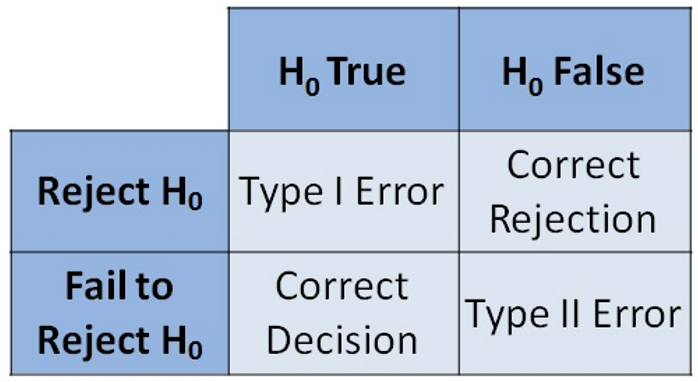
\includegraphics[width=0.5\linewidth]{/Users/craig.starbuck/Library/Mobile Documents/com~apple~CloudDocs/Documents/People Analytics Book/GitHub/peopleanalytics_lifecycle_book/graphics/hypothesis_testing_errors} 

}

\caption{Type I and II Errors}\label{fig:hyp-errs}
\end{figure}

\hypertarget{p-values}{%
\subsection{P-Values}\label{p-values}}

In statistical tests, the \textbf{p-value} is referenced to determine whether the null hypothesis can be rejected. The p-value represents the probability of obtaining a result at least as extreme as the one observed if the null hypothesis is true. As a general rule, if \(p\) \textless{} .05, we can confidently reject the null hypothesis and conclude that the observed difference or relationship was unlikely a chance observation.

While statistical significance helps us understand the probability of observing results by chance when there is no difference or effect in the population, it does not tell us anything about the size of the difference or effect. Analysis should never be reduced to inspecting p-values; in fact, p-values have been the subject of much controversy among researchers and practitioners in recent years. Later chapters will cover how to interpret results of statistical tests to surface the story and determine if there is anything `practically' significant among statistically significant findings.

\hypertarget{bonferroni-correction}{%
\subsection{Bonferroni Correction}\label{bonferroni-correction}}

One caveat when leveraging a p-value to determine statistical significance is that when multiple testing is performed -- that is, multiple tests using the same sample data -- the probability of a Type I error increases by a factor equivalent to the number of tests performed. It's important to note that there is not agreement among statisticians about how (or even whether) the p-value threshold for statistical significance needs to be adjusted to account for this increased risk. Nevertheless, we will cover this conservative approach for mitigating this risk.

Thus far, we have only discussed statistical significance in the context of a \textbf{per analysis error rate} -- that is, the probability of committing a Type I error for a single statistical test. However, when two or more tests are being conducted on the same sample, the \textbf{familywise error rate} is an important factor in determining statistical significance. The familywise error rate reflects the fact that as we conduct more and more analyses on the same sample, the probability of a Type I error across the set (or family) of analyses increases. The familywise error rate can be calculated by:

\[ \alpha_{FW} = 1 - (1 - \alpha_{PC})^C,  \]

where \(c\) is equal to the number of comparisons (or statistical tests) performed, and \(\alpha_{PC}\) is equal to the specified per analysis error rate (usually .05). For example, if \(\alpha\) = .05 per analysis, the probability of a Type I error with three tests on the same data increases from 5\% to 14.3\%: \(1 - (1 - .05)^3 = .143\).

The most common method of adjusting the familywise error rate down to the specified per analysis error rate is the \textbf{Bonferroni Correction}. To implement this correction, we can simply divide \(\alpha\) by the number of analyses performed on the dataset -- such as \(\alpha / 3 = .017\) in the case of three analyses with \(\alpha = .05\). This means that for each statistical test, we must achieve \(p < .017\) to report a statistically significant result. An alternative which allows us to achieve the same number of statistically significant results is to multiply the unadjusted per analysis p-values for each statistical test by the number of tests. For example, if we run three statistical tests and receive \(p = .014\), \(p = .047\), and \(p = .125\), we would achieve one significant result with the first method (\(p < .017\)) as well as with the alternative since the first statistical test satisfies the per analysis error rate (\(p < .05\)): \(p = .014 * 3 = .042\).

Perneger (1998) is one of many who oppose the use of the Bonferroni Correction, suggesting that these ``adjustments are, at best, unnecessary and, at worst, deleterious to sound statistical inference.'' The Bonferroni Correction is controversial among researchers because while applying the correction reduces the chance of a Type I error, it also increases the chance of a Type II error. Because this correction makes it more difficult to detect significant results, it is rare to find such a correction reported in published research, though research often involves multiple testing on the same sample. Perneger suggests that simply describing the statistical tests that were performed, and why, is sufficient for dealing with potential problems introduced by multiple testing.

\hypertarget{parametric-vs.nonparametric-tests}{%
\section{Parametric vs.~Nonparametric Tests}\label{parametric-vs.nonparametric-tests}}

\textbf{Parametric statistics} assume the population is normally distributed. \textbf{Nonparametric statistics} do not assume anything about the population parameters or distribution and are, therefore, often referred to as distribution free tests. Assuming the normality assumption holds, parametric tests generally have more power than their nonparametric counterparts. This means that with a nonparametric test, we are less likely to reject the null hypothesis when it is false if the data come from normally distributed populations.

Since the mean (expected value) is the most common measure of central tendency, parametric tests usually focus on comparing the mean or variance of data. You may recall that \(\mu\) and \(\sigma\) are sufficient to characterize a population distribution when data are situated symmetrically around the mean. However, the mean can be sensitive to outliers. If outliers are present in the data, the median may be a better way of representing the central tendency of data; in this case, nonparametric tests may be more appropriate.

In addition to normally distributed data in the population, and ensuring outliers are not materially influencing the mean, parametric tests also assume \textbf{homogeneity of variance} and \textbf{independence}. Homogeneity of variance assumes the variances across multiple groups are equal, though parametric tests are generally robust to violations of equal variances when the sample sizes are large. The assumption of independence requires observations to be randomly sampled from the population and independent of one another; that is, the value of one observation does not influence or depend on the value of another.

Spearman's correlation coefficient, which we used to evaluate the relationship between job level and education in Chapter \ref{uni-bi-stats}, is a nonparametric test since ordinal data are usually not normally distributed in the population. There is a nonparametric equivalent for each parametric test, and these will be reviewed in detail in Chapter \ref{aod}.

It's important to remember that the normal distribution properties under the CLT relate to the sampling distribution of means -- not to the distribution of the population or to the data for one individual sample. The CLT is important for estimating population parameters, but it does not transform a population distribution from nonnormal to normal. If we know the population distribution is nonnormal (e.g., ordinal, nominal, or skewed data), nonparametric tests should be leveraged.

\hypertarget{exercises-3}{%
\section{Exercises}\label{exercises-3}}

\begin{enumerate}
\def\labelenumi{\arabic{enumi}.}
\item
  Which of the following is an example of a null hypothesis, where \(\mu\) reflects the mean of a population?
  A. \(\mu_A = \mu_B\)
  B. \(\mu_A \neq \mu_B\)
  C. \(\mu_A < \mu_B\)
  D. \(\mu_A > \mu_B\)
  E. None of the above; all are examples of alternative hypotheses.
\item
  Which of the following describes a Type I Error?
  A. Failing to reject the null hypothesis when it is false
  B. Rejecting the null hypothesis when it is true
  C. Reporting something as significant when nothing of significance is present (a shame)
  D. Failing to detect something of significance (a pity)
  E. Both B and C
  F. Both A and D
\item
  The primary purpose of inferential statistics is to make inferences about a population based on sample data. Inferential statistics allows these inferences to be made with defined levels of confidence that what is observed in a sample is also characteristic of the larger population.
  A. True
  B. False
\item
  A T-Test should be used when \(\sigma\) is unknown and/or \(n\) \textless{} 30.
  A. True
  B. False
\item
  Randomness is essential to probabilistic methods.
  A. True
  B. False
\item
  Which of the following is characteristic of the Bonferroni Correction?
  A. Reducing the risk of a Type I Error
  B. Increasing the risk of a Type II Error
  C. Reducing the familywise error rate
\item
  Tolerance for a wider interval is an important tradeoff decision when increasing the level of confidence that a range of values contains an unknown population parameter.
  A. True
  B. False
\item
  A \(CI\) represents the range of values we expect to include an unknown population parameter (often the mean) for a specified degree of confidence.
  A. True
  B. False
\item
  When population parameters are unknown, which of the following tests is most appropriate for testing \(\mu_A = \mu_B\)?
  A. Z-Test
  B. T-Test
  C. Bayes' Theorem
  D. P-Test
\item
  According to the Empirical Rule, 95\% of normally distributed data lie within how many standard deviations of the mean?
  A. 1
  B. 2
  C. 3
  D. 4
\end{enumerate}

\hypertarget{data-prep}{%
\chapter{Data Preparation}\label{data-prep}}

\hypertarget{data-wrangling}{%
\section{Data Wrangling}\label{data-wrangling}}

\hypertarget{sql}{%
\subsection{SQL}\label{sql}}

\hypertarget{data-imputation}{%
\section{Data Imputation}\label{data-imputation}}

\hypertarget{feature-engineering}{%
\section{Feature Engineering}\label{feature-engineering}}

Level one people analytics tends to utilize only the delivered fields from the HRIS (e.g., location, job profile, org tenure, etc.), but a good next step is to derive smarter variables from these fields. These can then be used to slice and dice turnover and engagement data differently, use as inputs in attrition risk models, etc. Below are some ideas to get you started:

\begin{itemize}
\tightlist
\item
  Number of jobs per unit of tenure (larger proportions tend to see greater career pathing)
\item
  Office/remote worker (binary variable dummy coded as 1/0)
\item
  Local/remote manager (binary variable dummy coded as 1/0)
\item
  Hire/Rehire (binary variable dummy coded as 1/0)
\item
  Hired/acquired (proxy for culture shock effects)
\item
  Gender isolation (ratio of employee's gender to number of the same within immediate work
  group)
\item
  Generation isolation (comparison of age bracket to most frequent generational bracket within
  immediate work group)
\item
  Ethnic isolation (ratio of employee's ethnicity to number of the same within immediate work
  group)
\item
  Difference between employee and manager age
\item
  Percentage change between last two performance appraisal scores (per competency and/or
  overall)
\item
  Team and department quit outbreak indicators (ratio of terms over x months relative to average
  headcount over x months)
\item
  Industry experience (binary or length in years)
\end{itemize}

Remember to compute variables consistent with a need (e.g., is there reason to believe generationally isolated employees are more likely to term?). There may be a time and place for undertaking data mining initiatives with no a priori theories about what may be uncovered; however, more often than not, our efforts should be tied to specific hypotheses the business needs tested, which have sound theoretical underpinnings.

\hypertarget{exercises-4}{%
\section{Exercises}\label{exercises-4}}

\hypertarget{aod}{%
\chapter{Analysis of Differences}\label{aod}}

\hypertarget{comparing-2-distributions}{%
\section{Comparing 2 Distributions}\label{comparing-2-distributions}}

\hypertarget{comparing-3-distributions}{%
\section{Comparing 3+ Distributions}\label{comparing-3-distributions}}

\hypertarget{exercises-5}{%
\section{Exercises}\label{exercises-5}}

\hypertarget{lm}{%
\chapter{Linear Regression}\label{lm}}

It's important to draw a distinction between inferential and predictive models. Inferential models are highly interpretable and their utility is largely in understanding the nature and magnitude of the effect variables have on outcomes. Inferential models also lend to quantifying the extent to which we can generalize the observed effects to the larger population from which the sample was drawn. The objective in predictive modeling is to also to learn from patterns in historical data but for the purpose of achieving the most accurate predictions of future events -- even at the expense of interpretability. To be clear, this isn't to say that predictive models cannot be interpreted -- they certainly can -- but I've seen relatively few applications for predictive modeling in people analytics because models generally need to be highly interpretable to support action planning.

This chapter is dedicated to inferential models to support a working understanding of how to interpret model output and communicate clear, data-driven narratives that respect the nuance and noise characteristic of people data. The following chapter will provide an overview of predictive modeling frameworks.

Regression is perhaps the most important statistical learning technique for people analytics. If you have taken a statistics course at the undergraduate or graduate levels, you have surely already encountered it. Before diving into the math to understand the mechanics of regression, let's develop an intuitive understanding.

Imagine we are sitting at a large public park in NYC on a nice fall afternoon. If asked to estimate the annual compensation of the next person to walk by, in the absence of any additional information how would you estimate this? Most would likely estimate the average annual compensation of everyone capable of walking by. Since this would include both residents and visitors, this would be a very large group of people! The obvious limitation with this approach is that among the large group of people capable of walking by, there is likely a significant range of annual compensation values. Many walking by may be children, unemployed, or retirees who earn no annual compensation, while others may be highly compensated senior executives at the pinnacle of their careers. Since the range of annual compensation could be zero to billions of dollars, estimating the average of such a large population is likely going to be highly inaccurate without more information about who may walk by.

Let's consider that we are sitting outside on a weekday afternoon. Should this influence our annual compensation estimate? It is likely that we can eliminate a large segment of those likely to walk by, as we would expect most children to be in school on a typical fall weekday afternoon. It's also unlikely that those who are employed and not on vacation will walk by on a fall weekday afternoon. Therefore, factoring in that it is a weekday should limit the size of the population which in turn may reduce the range of annual compensation values for our population of passerbys.

Let's now consider that the park is open only to invited guests for a symposium on people analytics. Though it may be difficult to believe, a relatively small subset of the population is likely interested in attending such a symposium, so this information will likely be very helpful in reducing the size of the population who could walk by, which should further reduce the range of annual compensation since we probably have a good idea of the profile of those most likely to attend. This probably also lessens (or altogether eliminates) the importance of the weekday factor in explaining why people vary in the amount of compensation they earn each year.

Furthermore, let's consider that only those who reside in NYC and Boise were invited, and that the next person to walk by resides in Boise. Most companies apply a significant cost of living multiplier to the compensation for those in an expensive region such as NYC, resulting in a significant difference in compensation relative to those residing in a much less expensive city like Boise -- all else being equal. Therefore, if we can partition attendees into two groups based on their geography, this should limit the range of annual compensation significantly within each -- likely making the average compensation amount in each group a more nuanced and reasonable estimate.

What if we also learn the specific zip code in which the next passerby from Boise resides? The important information is likely captured in the larger city label (NYC vs.~Boise), and the compensation for the specific zip codes within each city are unlikely to vary to a significant degree. Assuming this is true, it probably would not make sense to consider both the city name and zip code since they are effectively redundant pieces of information with regard to explaining differences in annual compensation.

What if we learn that the next person to walk by will be wearing a blue shirt? Does this influence your estimate? Unless there is research to suggest shirt color and earnings are related, this information will likely not contribute any significant information to our understanding of why people vary in the amount of compensation they earn annually and should, therefore, not be considered.

You can probably think of many relevant variables that would help further narrow the range of annual compensation. These may include job, level, years of experience, education, location, among other factors. The main thing to understand is that for each group of observations with the same characteristics -- such as senior analysts with a graduate degree who reside in NYC -- there is a distribution of annual compensation. This distribution reflects unexplained variance. That is, we do not have information to explain why the compensation for each and every person is not the same and in social science contexts, it simply is not practical to explain 100 percent of the variance in outcomes. Two people may be similar on hundreds of factors (experience, education, skills) but one was simply a more effective negotiator when offered the same role and commanded a higher salary. It's likely we do not have data on salary negotiation ability so this information would leave us with unexplained variance in compensation. The goal is simply to identify the variables that provide the most information in helping us tighten the distribution so that estimating the average value will generally be an accurate estimate for those in the larger population with the same characteristics.

While we can generally improve our estimates with more relevant information (not shirt color or residential zip code in this case), it is important to understand that samples which are too small (n \textless{} 30) lend to anomalies; modeling noise in sparse data can result in models that are unlikely to generalize beyond the sample data. For example, if the only people from Boise to attend the people analytics symposium happen to be two ultra wealthy tech entrepreneurs who earn millions each year, it would not be appropriate to use this as the basis for our estimates of all future attendees from Boise. This is a phenomenon known as overfitting that will be covered later in this chapter.

This is the essence of regression modeling: find a limited number of variables which independently or jointly provide significant information that helps explain (by reducing) variance around the average value. As illustrated in this example, adding additional variables (information) can impact the importance of other variables or may offer no incremental information at all. In the subsequent sections, we will cover how to identify which variables are important and how to quantify the effect they have on the outcome.

\hypertarget{simple-linear-regression}{%
\section{Simple Linear Regression}\label{simple-linear-regression}}

\hypertarget{parameter-estimation}{%
\subsection{Parameter Estimation}\label{parameter-estimation}}

Ordinary Least Squares (OLS) is the most common method for estimating unknown parameters in a linear regression model.

\hypertarget{multiple-linear-regression}{%
\section{Multiple Linear Regression}\label{multiple-linear-regression}}

\hypertarget{moderation}{%
\subsection{Moderation}\label{moderation}}

\hypertarget{mediation}{%
\subsection{Mediation}\label{mediation}}

\hypertarget{polynomial-regression}{%
\section{Polynomial Regression}\label{polynomial-regression}}

\hypertarget{hierarchical-models}{%
\section{Hierarchical Models}\label{hierarchical-models}}

\hypertarget{exercises-6}{%
\section{Exercises}\label{exercises-6}}

\hypertarget{glm}{%
\chapter{Generalized Linear Regression}\label{glm}}

\hypertarget{logistic-regression}{%
\section{Logistic Regression}\label{logistic-regression}}

Logistic regression is an excellent tool when the outcome is categorical. Logistic regression allows us to model the probability of different classes -- a type of modeling often referred to as classification. The context for classification can be binomial for two classes (e.g., active/inactive, promoted/not promoted), multinomial for multiple unordered classes (e.g., skills, job families), or ordinal for multiple ordered classes (e.g., survey items measured on a Likert scale, performance level).

\hypertarget{binomial-logistic-regression}{%
\subsection{Binomial Logistic Regression}\label{binomial-logistic-regression}}

\hypertarget{multinomial-logistic-regression}{%
\subsection{Multinomial Logistic Regression}\label{multinomial-logistic-regression}}

\hypertarget{ordinal-logistic-regression}{%
\subsection{Ordinal Logistic Regression}\label{ordinal-logistic-regression}}

\hypertarget{proportional-odds-logistic-regression}{%
\subsection{Proportional Odds Logistic Regression}\label{proportional-odds-logistic-regression}}

\hypertarget{poisson-regression}{%
\section{Poisson Regression}\label{poisson-regression}}

\hypertarget{exercises-7}{%
\section{Exercises}\label{exercises-7}}

\hypertarget{surv-anal}{%
\chapter{Survival Analysis}\label{surv-anal}}

\hypertarget{exercises-8}{%
\section{Exercises}\label{exercises-8}}

\hypertarget{pred-mod}{%
\chapter{Predictive Models}\label{pred-mod}}

\hypertarget{bias-variance-trade-off}{%
\section{Bias-Variance Trade-Off}\label{bias-variance-trade-off}}

\hypertarget{cross-validation}{%
\section{Cross-Validation}\label{cross-validation}}

\hypertarget{balancing-classes}{%
\section{Balancing Classes}\label{balancing-classes}}

\hypertarget{model-performance}{%
\section{Model Performance}\label{model-performance}}

\hypertarget{automated-machine-learning-automl}{%
\section{Automated Machine Learning (AutoML)}\label{automated-machine-learning-automl}}

\hypertarget{exercises-9}{%
\section{Exercises}\label{exercises-9}}

\hypertarget{unsup-lrn}{%
\chapter{Unsupervised Learning}\label{unsup-lrn}}

\hypertarget{factor-analysis}{%
\section{Factor Analysis}\label{factor-analysis}}

\hypertarget{clustering}{%
\section{Clustering}\label{clustering}}

\hypertarget{exercises-10}{%
\section{Exercises}\label{exercises-10}}

\hypertarget{net-anal}{%
\chapter{Network Analysis}\label{net-anal}}

\hypertarget{centrality-measures}{%
\section{Centrality Measures}\label{centrality-measures}}

\textbf{Degree Centrality}

\textbf{Eigenvector Centrality}

\textbf{Betweenness Centrality}

\textbf{Closeness Centrality}

\hypertarget{exercises-11}{%
\section{Exercises}\label{exercises-11}}

\hypertarget{data-viz}{%
\chapter{Data Visualization}\label{data-viz}}

\hypertarget{design-guidelines}{%
\section{Design Guidelines}\label{design-guidelines}}

\hypertarget{visualization-types}{%
\section{Visualization Types}\label{visualization-types}}

\hypertarget{tables}{%
\subsection{Tables}\label{tables}}

\hypertarget{heatmaps}{%
\subsection{Heatmaps}\label{heatmaps}}

\hypertarget{scatterplots}{%
\subsection{Scatterplots}\label{scatterplots}}

\hypertarget{line-graphs}{%
\subsection{Line Graphs}\label{line-graphs}}

\textbf{Single Series}

\textbf{Two Series}

\textbf{Multiple Series}

\hypertarget{slopegraphs}{%
\subsection{Slopegraphs}\label{slopegraphs}}

\hypertarget{bar-charts}{%
\subsection{Bar Charts}\label{bar-charts}}

\textbf{Vertical}

\textbf{Horizontal}

\textbf{Stacked}

\hypertarget{waterfall-charts}{%
\subsection{Waterfall Charts}\label{waterfall-charts}}

\hypertarget{area-charts}{%
\subsection{Area Charts}\label{area-charts}}

\hypertarget{pie-charts}{%
\subsection{Pie Charts}\label{pie-charts}}

\hypertarget{exercises-12}{%
\section{Exercises}\label{exercises-12}}

\hypertarget{storytelling}{%
\chapter{Data Storytelling}\label{storytelling}}

\hypertarget{know-your-audience}{%
\section{Know Your Audience}\label{know-your-audience}}

\hypertarget{tldr}{%
\section{TL;DR}\label{tldr}}

\hypertarget{telling-the-story}{%
\section{Telling the Story}\label{telling-the-story}}

\hypertarget{reference-material}{%
\section{Reference Material}\label{reference-material}}

\hypertarget{exercises-13}{%
\section{Exercises}\label{exercises-13}}

\hypertarget{bibli}{%
\chapter{Bibliography}\label{bibli}}

Albright, S. C., \& Winston, W. L. (2016). Business Analytics: Data Analysis \& Decision Making (6th ed.). Boston, MA: Cengage.

Baron, R. M., \& Kenny, D. A. (1986). The moderator--mediator variable distinction in social psychological research: Conceptual, strategic, and statistical considerations. Journal of Personality and Social Psychology, 51(6), 1173--1182.

Bartlett, R. (2013). A Practitioner's Guide to Business Analytics: Using Data Analysis Tools to Improve Your Organization's Decision Making and Strategy. New York, NY: McGraw-Hill.

Creswell, J. W., \& Creswell, J. D. (2018). Research Design: Qualitative, Quantitative, and Mixed Methods Approaches (5th ed.). Los Angeles: Sage.

Daw, R. H., \& Pearson, E. S. (1972). Studies in the History of Probability and Statistics. XXX. Abraham De Moivre's 1733 Derivation of the Normal Curve: A Bibliographical Note. Biometrika, 59(3), 677--680. \url{https://doi.org/10.2307/2334818}

DeVellis, R. F. (2012). Scale development: Theory and applications. Thousand Oaks, Calif: Sage.

James, G., Witten, D., Hastie, T., \& Tibshirani, R. (2013). An Introduction to Statistical Learning: With Applications in R. New York: Springer.

Kahneman, D. (2011). Thinking, fast and slow. New York: Farrar, Straus and Giroux.

Kerlinger, F., \& Lee, H. (2000). Foundations of behavioral research (4th ed.). Melbourne: Wadsworth.

Perneger, T. V. (1998). What's wrong with Bonferroni adjustments. BMJ, 316(7139), 1236-1238.

Pishro-Nik, H. (2014). Introduction to Probability: Statistics and Random Processes. Blue Bell, PA: Kappa Research, LLC.

Wheelan, C. (2013). Naked Statistics: Stripping the Dread from the Data. New York: W.W. Norton.

\hypertarget{appendix}{%
\chapter{Appendix}\label{appendix}}

\hypertarget{exercise-solutions}{%
\section{Exercise Solutions}\label{exercise-solutions}}

\textbf{Measurement \& Sampling}

\begin{enumerate}
\def\labelenumi{\arabic{enumi}.}
\item
  Parameters are descriptions or characteristics of a sample, while statistics are descriptions or characteristics of a population.
  B. False
\item
  How does a sampling frame differ from a sample?

  A sampling frame represents the subset of the population to which the researcher has access, while the sample is the subset of the sampling frame that ultimately participates in the research.
\item
  How does cluster sampling differ from stratified random sampling?

  It is the \emph{clusters} that are selected at random with cluster sampling rather than the \emph{individuals} with stratified random sampling.
\item
  What is the primary benefit of probabilistic sampling methods over non-probabilistic sampling?

  Probability sampling allows us to make inferences about a larger population based on sample data, while this is not the case for non-probability sampling methods since the sample is unlikely to be representative of the population.
\item
  Nonresponse bias is only applicable in the context of surveys.
  B. False
\item
  Which of the following variable types influences the strength of the effect one variable has on another?
  C. Moderating Variable
\item
  100 randomly selected employees in the Marketing department of an organization participated in a survey on career pathing for marketing professionals. What is the sample and what is the population sampled in this case?
  B. Sample: 100 employees who completed the survey, Population: Marketing employees
\item
  Zero represents the absence of something for inveral scaled variables, whereas this is not the case for ratio scaled variables.
  B. False
\item
  Discrete variables can have more than 2 values.
  A. True
\item
  Which of the following are NOT probabilistic sampling methods?
  B. Quota sampling
  D. Purposive sampling
\end{enumerate}

\textbf{Research Fundamentals}

\begin{enumerate}
\def\labelenumi{\arabic{enumi}.}
\tightlist
\item
  What type of research method and design would be best suited for a study aiming to understand the effect of stay interviews on employee attrition?
\end{enumerate}

A quantitative research method and quasi-experimental design would be best suited for this study. While experimental designs are more rigorous than quasi-experiments, stay interviews are unlikely to be initiated via random processes; leaders will likely identify select people as having a higher risk of attrition and initiate stay interviews accordingly.

\begin{enumerate}
\def\labelenumi{\arabic{enumi}.}
\setcounter{enumi}{1}
\tightlist
\item
  Why are quasi-experiments less rigorous than true experiments?
\end{enumerate}

Randomized experimental designs provide the most rigor with regard to causal validity, but random assignment is not performed in a quasi-experimental context.

\begin{enumerate}
\def\labelenumi{\arabic{enumi}.}
\setcounter{enumi}{2}
\tightlist
\item
  Why aren't experimental designs always implemented when an experimenter-manipulated IV is warranted?
\end{enumerate}

Randomized experimental designs provide the most rigor with regard to causal validity. However, in social science research contexts, true experiments often are not possible due to ethical considerations.

\begin{enumerate}
\def\labelenumi{\arabic{enumi}.}
\setcounter{enumi}{3}
\tightlist
\item
  What is the role of research questions?
\end{enumerate}

Research questions help focus the study, determine the appropriate methodology, and guide each stage of inquiry, analysis, and reporting.

\begin{enumerate}
\def\labelenumi{\arabic{enumi}.}
\setcounter{enumi}{4}
\tightlist
\item
  What is the role of research hypotheses?
\end{enumerate}

Research hypotheses are testable statements about the expected outcome of a research project or experiment.

\begin{enumerate}
\def\labelenumi{\arabic{enumi}.}
\setcounter{enumi}{5}
\tightlist
\item
  What is the difference between internal and external validity, and why are these concepts important in research?
\end{enumerate}

Internal validity reflects the robustness of the study -- the extent to which confounding variables are controlled. External validity refers to the extent to which study conclusions will hold in other contexts (for other people, in other places, at other times). Confidence in conclusions about causal effects or statistical relationships, and the likelihood of such conclusions to hold true in other contexts, is rooted in a study's internal and external validity.

\begin{enumerate}
\def\labelenumi{\arabic{enumi}.}
\setcounter{enumi}{6}
\tightlist
\item
  What is an example of a mixed methods study?
\end{enumerate}

One example of a mixed methods study is a two-part study in which part 1 involves employee focus groups to surface themes that are top-of-mind for employees, and part 2 involves a survey to measure constructs related to the emergent themes in order to test statistical relationships with outcomes like engagement and retention.

\begin{enumerate}
\def\labelenumi{\arabic{enumi}.}
\setcounter{enumi}{7}
\tightlist
\item
  What is the key difference between experimental and non-experimental research designs?
\end{enumerate}

Unlike experimental designs, non-experiments do not involve the manipulation of an IV. The goal of non-experiments is not to provide evidence for causal effects, but to study measured variables as they naturally occur.

\begin{enumerate}
\def\labelenumi{\arabic{enumi}.}
\setcounter{enumi}{8}
\tightlist
\item
  What are the differences between cross-sectional, correlational, and observational non-experimental designs?
\end{enumerate}

Cross-sectional research compares two or more natural groups of people. Correlational research involves studying the statistical relationship between two variables. Observational research refers to studies in which the researcher gathers information without research subjects being explicitly involved in the recording of data.

\begin{enumerate}
\def\labelenumi{\arabic{enumi}.}
\setcounter{enumi}{9}
\tightlist
\item
  What is an example of an A/B testing use case in people analytics?
\end{enumerate}

One example of an A/B testing use case for people analytics is dashboard user experience (UX) testing -- displaying multiple versions of a dashboard to users to study usage patterns and optimize the UX.

\textbf{Univariate \& Bivariate Analysis}

\begin{enumerate}
\def\labelenumi{\arabic{enumi}.}
\item
  Which of the following measures of central tendency is least sensitive to extreme values (outliers)?
  A. Median
\item
  The standard deviation represents the `average' amount by which \(x\) values deviate (or vary) from the mean. A large standard deviation indicates there is considerable spread in the data, whereas a small standard deviation indicates the mean is fairly representative of the data.
  A. True
\item
  A positively skewed distribution has its largest allocation to the left and a negative distribution to the right.
  B. False
\item
  Large covariance coefficients always indicate strong bivariate associations.
  B. False
\item
  Which of the following can be found in boxplots?
  A. Quartiles
  B. Median
  D. IQR
  E. Outliers
\item
  The 3rd quartile (Q3) is equivalent to the 75th percentile.
  A. True
\item
  Which of the following correlation coefficients can be used when evaluating the relationship between a pair of rank-ordered variables?
  B. Spearman's Rank
  E. Kendall's Rank
\item
  Which of the following correlation coefficients can be used when evaluating the relationship between a pair of dichotomous variables?
  C. Phi
\item
  Platykurtic distributions are flat relative to mesokurtic distributions.
  A. True
\item
  When using the Pearson method, values down the diagonal of a covariance matrix represent the variance for each variable.
  A. True
\end{enumerate}

\textbf{Inferential Statistics}

\begin{enumerate}
\def\labelenumi{\arabic{enumi}.}
\item
  Which of the following is an example of a null hypothesis, where \(\mu\) reflects the mean of a population?
  A. \(\mu_A = \mu_B\)
\item
  Which of the following describes a Type I Error?
  E. Both B and C
\item
  The primary purpose of inferential statistics is to make inferences about a population based on sample data. Inferential statistics allows these inferences to be made with defined levels of confidence that what is observed in a sample is also characteristic of the larger population.
  A. True
\item
  A T-Test should be used when \(\sigma\) is unknown and/or \(n\) \textless{} 30.
  A. True
\item
  Randomness is essential to probabilistic methods.
  A. True
\item
  Which of the following is characteristic of the Bonferroni Correction?
  A. Reducing the risk of a Type I Error
  B. Increasing the risk of a Type II Error
  C. Reducing the familywise error rate
\item
  Tolerance for a wider interval is an important tradeoff decision when increasing the level of confidence that a range of values contains an unknown population parameter.
  A. True
\item
  A \(CI\) represents the range of values we expect to include an unknown population parameter (often the mean) for a specified degree of confidence.
  A. True
  B. False
\item
  When population parameters are unknown, which of the following tests is most appropriate for testing \(\mu_A = \mu_B\)?
  B. T-Test
\item
  According to the Empirical Rule, 95\% of normally distributed data lie within how many standard deviations of the mean?
  B. 2
\end{enumerate}

\hypertarget{d-framework-1}{%
\section{4D Framework}\label{d-framework-1}}

\begin{figure}
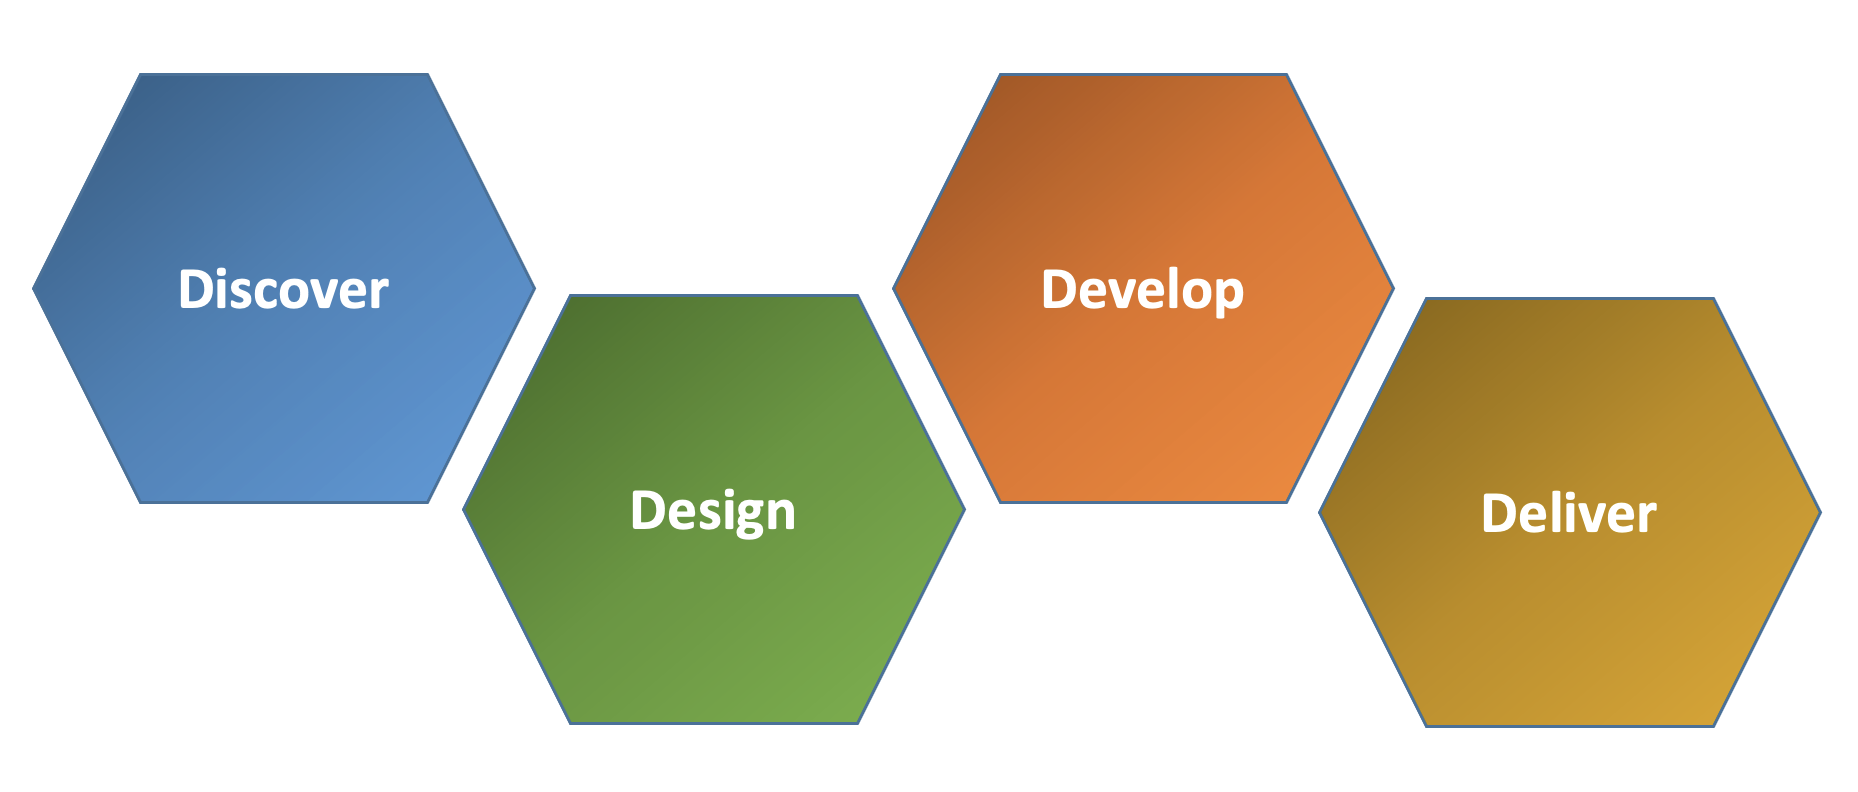
\includegraphics[width=0.75\linewidth]{/Users/craig.starbuck/Library/Mobile Documents/com~apple~CloudDocs/Documents/People Analytics Book/GitHub/peopleanalytics_lifecycle_book/graphics/4d_framework} \caption{Figure 1: 4D Framework}\label{fig:4d-overview}
\end{figure}

1. Discover

You are likely familiar with the old adage: ``An ounce of prevention is worth a pound of cure.'' Such is the case with respect to planning in an analytics context. During the Discover phase, it is important to remain in the problem zone; seek to understand your clients' needs through active listening and questions. This is not the time for solutioning or committing to any specific deliverables. If the client's needs are ambiguous, proceeding will likely be an exercise in futility. Outlined below is a set of general questions that should be considered during this initial phase to prevent allocating scarce time and resourcing to a project that ultimately misses the mark.

\begin{itemize}
\item
  Client

  Who is the client? A client can be a person or organization that has contracting you for consulting services, or an internal stakeholder within your organization who has need. What is important to them?
\item
  Primary Objective

  \begin{itemize}
  \tightlist
  \item
    What is the client ultimately hoping to accomplish?
  \item
    Is the request merely to satisfy one's curiosity, or are there actions that can realistically be taken to materially influence said objective?
  \end{itemize}
\item
  Problem Statement

  \begin{itemize}
  \tightlist
  \item
    One of my most important early steps is clearly defining the problem statement. If your understanding of the problem -- after translating from the business terms in which it was initially expressed -- is misaligned with the client's needs, none of the subsequent steps matter.
  \end{itemize}
\item
  Guiding Theories

  \begin{itemize}
  \tightlist
  \item
    What theoretical explanations can the client offer as potential rationalizations for the phenomena of interest?
  \item
    Are there existing theories in the organizational literature that should guide how the problem is tackled (e.g., findings from similar research implemented in other contexts)?
  \end{itemize}
\item
  Research Questions

  To respect the nuances of the problem statement, it is important to unpack it and frame as a set of overarching questions to guide the research.

  \begin{itemize}
  \tightlist
  \item
    Q1: \ldots{}
  \item
    Q2: \ldots{}
  \item
    Q3: \ldots{}
  \end{itemize}
\item
  Research Hypotheses

  Once research questions are developed, what do you expect to find based on anecdotal stories or empirical findings? As a next step, these expectations should be expressed in the form of research hypotheses. Please note that these research hypotheses are different from statistical hypotheses.

  \begin{itemize}
  \tightlist
  \item
    H1: \ldots{}
  \item
    H2: \ldots{}
  \item
    H3: \ldots{}
  \end{itemize}

  To ensure the hypotheses lend themselves to actionable analyses, it is important to consider the following: ``What does success look like?'' In other words, once the project is complete, against which success measures will the project's success be determined? Curiosity is not a business reason and hope is not a reasonable strategy. The following questions may prove helpful in the promotion of actionable -- over merely interesting outcomes:

  \begin{itemize}
  \tightlist
  \item
    What will be done if the hypotheses are empirically supported?
  \item
    What will be done if the hypotheses are not empirically supported?
  \end{itemize}
\item
  Assumptions

  At this point, it's helpful to consider what assumptions may be embedded in this discovery work. Are the questions and hypotheses rooted in what the client has theorized, or are these the product of an ambiguous understanding of the client's needs?
\item
  Cadence

  \begin{itemize}
  \tightlist
  \item
    Is this analysis a one-off, or could there be a need to refresh this analysis on a regular cadence?
  \item
    Are there dates associated with programs, actions, etc. this analysis is intended to support?
  \end{itemize}
\item
  Aggregation

  Is there a need for individual-level detail supporting the analysis? Aaggregate data should generally be the default unless a compelling justification exists and approval from legal and privacy partners is granted. One important role of analysts is to help keep the audience focused on the bigger picture and findings. Access to individual-level detail can not only introduce unnecessary legal and compliance risk but can also lead to questions and probing that can delay taking needed actions based on the results.
\item
  Deliverable

  What is the preferred method of communicating the results of the analysis (e.g., interactive dashboard, static slide deck, document)? It is important to determine this early so that subsequent efforts can be structured to support the preferred deliverable. For example, if an interactive dashboard is preferred, does your Engineering department need to prioritize dependent tasks such as data feeds, row-level security, BI development, and production server migrations?
\item
  Filters \& Dimensions

  How does your client prefer to segment the workforce? Some common grouping dimensions are business unit, division, team, job family, location, tenure, and management level.
\end{itemize}

2. Design

Perhaps the most important initial question to answer in the design phase is: ``Does anything already exist that addresses part, or all, of the client's objectives?'' If the existing solution will suffice, it's possible that there is simply a communication/education gap, and you can allocate time and resources elsewhere.

The end-user experience is of paramount importance during the Design phase, as solutions should have a consistent look and feel regardless of who developed the product. To achieve this, it is important to resist siloed thinking and consider the broader set of analytics solutions the team has delivered -- or is in the process of delivering.

\begin{itemize}
\item
  Data Privacy

  Are there potential concerns with the study's objective, planned actions, and/or requested data elements from an employee privacy or legal perspective? A cross-functional data governance committee can help with efficient and consistent decisioning on requests for people data and analytics.
\item
  Data Sources \& Elements

  \begin{itemize}
  \tightlist
  \item
    What data sources are required?
  \item
    What data elements are required?
  \end{itemize}

  In cases where sensitive attributes such as gender, ethnicity, age, sexual orientation, and disability status are requested, it's always best to exercise a `safety first' mentality and consult with legal and privacy partners to ensure there is comfort with the intended use of the data. The decision on whether or not to include these sensitive data elements is often less about what the audience can view (e.g., People Partners may already have access to the information at the person level in the source system) and more anchored in what they plan to do with the information.

  Is the required data already accessible in a data warehouse or other analytics environment? If not, does it need to be? What is required to achieve this?
\item
  Data Quality

  It is important to understand the data generative process and never make assumptions about how anomalies or missing data should be interpreted. After identifying what data sources will be required for a particular analysis, it is important to meet with source system owners and data stewards to deeply understand the business processes by which data are generated in the system(s). Are there data quality concerns that need to be explored and addressed?
\item
  Variables

  How will the constructs be measured (e.g., survey instrument, derived attribute, calculated field)?
\item
  Analysis Method

  What are the appropriate analysis methods based on the research hypotheses? If modeling is required, is it more important to index on accuracy or interpretability?
\item
  Dependencies

  Are other teams required to develop this solution? What is the nature of the work each dependent team will perform? Are there required system configuration changes? Do these teams have capacity to support?
\item
  Change Management

  Will this solution impact current processes or solutions? If so, what is the change management plan to facilitate a seamless transition and user experience?
\item
  Sign-Off

  Generally, it is best for the client to signoff on the problem statement, analysis approach, and wire frame for the deliverable (if applicable) before providing an ETA and proceeding to the development phase. This ensures alignment on the client's needs and the perceived utility of the solution in addressing those needs.
\end{itemize}

3. Develop

\begin{itemize}
\item
  Development Patterns

  \begin{itemize}
  \tightlist
  \item
    Are there development patterns that should guide the development approach to support consistency?
  \item
    Are there existing calculated fields that can/should be leveraged for derived data?
  \item
    Are there best practices that should be employed to optimize performance (e.g., load time for dashboards, executing complex queries during non-peak times)?
  \item
    Are there standard color palettes that should be applied?
  \end{itemize}
\item
  Productionalizable Code

  \begin{itemize}
  \tightlist
  \item
    How do models and data science pipelines need to be developed to facilitate a seamless migration from lower to upper environments? For example, initial exploratory data analysis (EDA) may be performed using curated data in flat files for the purpose of identifying meaningful trends, relationships, and differences, but where will this data need to be sourced in production to automate the refresh of models at a regular interval? If the data were provided from multiple source systems, what joins are required to integrate the data? What transformation logic or business rules need to be applied to reproduce the curated data?
  \end{itemize}
\item
  Unit Testing

  \begin{itemize}
  \tightlist
  \item
    What test cases will ensure the veracity of data?
  \item
    Who will perform the testing?
  \end{itemize}
\item
  UAT Testing

  \begin{itemize}
  \tightlist
  \item
    In the spirit of agility and constant contact with the client to prevent surprises, it is generally a good idea to have the client take the solution for a test run within the UAT environment and then provide sign-off before migrating to production. If the deliverable is a deck or doc with results from a model, UAT may surface clarifying questions that can be addressed before releasing to the broader audience.
  \end{itemize}
\end{itemize}

4. Deliver

The Deliver phase can take many forms depending on the solution being released. If the solution is designed for a large user base, a series of recorded trainings may be in order so that there is a helpful reference for those unable to attend the live sessions or new joiners in the future. It is important to monitor success measures, which could be insights aligned to research hypotheses, dashboard utilization metrics, or any number of others defined within the Discover phase.

\bibliography{book.bib}

\end{document}
